\documentclass{article}
\usepackage{natbib}
\setcitestyle{numbers,square,comma}
\usepackage{multirow}

% if you need to pass options to natbib, use, e.g.:
% \PassOptionsToPackage{numbers, compress}{natbib}
% before loading neurips_2025


% ready for submission
% \usepackage{neurips_2025}
% \usepackage{etoolbox}
% \newtoggle{isSubmission}
% \toggletrue{isSubmission}

% camera ready for arxiv
% \usepackage[preprint]{neurips_2025}
% \usepackage{etoolbox}
% \newtoggle{isSubmission}
% \togglefalse{isSubmission}

% camera ready for submission
\usepackage[final]{neurips_2025}
\usepackage{etoolbox}
\newtoggle{isSubmission}
\toggletrue{isSubmission}

% to compile a preprint version, e.g., for submission to arXiv, add add the
% [preprint] option:
    % \usepackage[preprint]{neurips_2025}


% to compile a camera-ready version, add the [final] option, e.g.:
%     \usepackage[final]{neurips_2025}


% to avoid loading the natbib package, add option nonatbib:
%    \usepackage[nonatbib]{neurips_2025}


\usepackage[utf8]{inputenc} % allow utf-8 input
\usepackage[T1]{fontenc}    % use 8-bit T1 fonts
\usepackage{hyperref}       % hyperlinks
\usepackage{url}            % simple URL typesetting
\usepackage{booktabs}       % professional-quality tables
\usepackage{amsfonts}       % blackboard math symbols
\usepackage{nicefrac}       % compact symbols for 1/2, etc.
\usepackage{microtype}      % microtypography
\usepackage[table]{xcolor}         % colors
\usepackage{amsmath}
\usepackage{float}
\usepackage[nameinlink]{cleveref}
\usepackage{enumitem}
% \usepackage{minitoc}
% \usepackage{etoc}
\usepackage{titletoc}
% \stopcontents[app]

% \titlecontents{section}
%   [0pt]                      % 保持默认左缩进
%   {}                         % 保持默认格式（不加粗等）
%   {\contentslabel{2.5em}}    % 保持默认章节编号格式
%   {}                         % 保持默认无编号格式
%   {\hfill\contentspage}      % 保持默认页码对齐
%   [\vspace{-0.6em}]          % 仅这一项：减少章节之间的垂直间距
  

\newcommand*{\affaddr}[1]{#1} 
\newcommand*{\affmark}[1][*]{\textsuperscript{#1}}
\newcommand{\authormark}[2][]{%
  \begingroup
  \def\@thefnmark{#1}%
  \footnote{#2}%
  \endgroup
}




% \title{BeamAlign: Likelihood-Based Search Enables Weak-to-Strong Alignment}
\title{Flow-GRPO: \\Training Flow Matching Models via Online RL}
% \title{Weak-to-Strong Search}

% The \author macro works with any number of authors. There are two commands
% used to separate the names and addresses of multiple authors: \And and \AND.
%
% Using \And between authors leaves it to LaTeX to determine where to break the
% lines. Using \AND forces a line break at that point. So, if LaTeX puts 3 of 4
% authors names on the first line, and the last on the second line, try using
% \AND instead of \And before the third author name.


% \author{%
%   Jie Liu$^*$, Gongye Liu$^*$, Jiajun Liang, Yangguang Li, Zhanhui Zhou, \\ \textbf{Jiaheng Liu, Xintao Wang, Pengfei Wan, Di Zhang, Wanli Ouyang{\dag}} \\
%   Shanghai Artificial Intelligence Laboratory \\
%   $^*$Equal Contribution, $^\dag$Corresponding Author \\
%   \texttt{jieliu@link.cuhk.edu.hk} \\
%   Code: \url{https://github.com/yifan123/flow-grpo}
% }
\author{%
\bf
Jie Liu\affmark[1,3,5]\thanks{Equal contribution, \textsuperscript{\dag}Corresponding author}~~~ 
Gongye Liu\affmark[2,3]\textsuperscript{*}~~~ 
Jiajun Liang\affmark[3]~~~ 
Yangguang Li\affmark[1]\\
\bf
Jiaheng Liu\affmark[4]~~~ 
Xintao Wang\affmark[3]~~~ 
Pengfei Wan\affmark[3]~~~ 
Di Zhang\affmark[3]~~~ 
Wanli Ouyang\affmark[1,5]\textsuperscript{\dag}\\
\affaddr{\affmark[1]MMLab, CUHK~~~~~~~~~~}
\affaddr{\affmark[2]Tsinghua University~~~~~~~~~~}
\affaddr{\affmark[3]Kling Team, Kuaishou Technology~~~~~~~~~~} \\
\affaddr{\affmark[4]Nanjing University~~~~~~~~~~} 
\affaddr{\affmark[5]Shanghai AI Laboratory} \\
\small
\texttt{jieliu@link.cuhk.edu.hk}~~~~~~  
\texttt{wlouyang@ie.cuhk.edu.hk}\\
Code: \url{https://github.com/yifan123/flow_grpo}
% \tt\small{Project page: \url{https://gongyeliu.github.io/StyleCrafter.github.io/}}\\
}

% customized packages and commands
\bibliographystyle{unsrt}
\usepackage{graphics}
\usepackage[table]{xcolor}
\usepackage{graphicx}
\usepackage{subcaption}
\usepackage{caption}
\usepackage{amssymb}
\usepackage{algorithm}
\usepackage{algpseudocode}
\usepackage{wrapfig}
\usepackage{longtable}
\usepackage{fancyvrb}
\usepackage{empheq}
\definecolor{metacolor}{HTML}{0064E0}
\hypersetup{
  colorlinks,
  linkcolor=metacolor,
  citecolor=metacolor,
  urlcolor=metacolor
}
\usepackage{adjustbox}
\usepackage{makecell} 
\definecolor{color_blue}{HTML}{E7EFFA}
\definecolor{color_green}{HTML}{E6F8E0}
\definecolor{color_gray}{HTML}{ECECEC}
\definecolor{pearDark}{HTML}{2980B9}

\input{commands/math}
% macro
\newcommand{\todo}[1]{\textcolor{orange}{TODO: #1}}


\begin{document}

% \dominitoc


\maketitle
\begin{abstract}
We propose Flow-GRPO, the first method to integrate online policy gradient reinforcement learning (RL) into flow matching models. Our approach uses two key strategies: (1) an ODE-to-SDE conversion that transforms a deterministic Ordinary Differential Equation (ODE) into an equivalent Stochastic Differential Equation (SDE) that matches the original model's marginal distribution at all timesteps, enabling statistical sampling for RL exploration; and (2) a Denoising Reduction strategy that reduces training denoising steps while retaining the original number of inference steps, significantly improving sampling efficiency without sacrificing performance.
Empirically, Flow-GRPO is effective across multiple text-to-image tasks. For compositional generation, RL-tuned SD3.5-M generates nearly perfect object counts, spatial relations, and fine-grained attributes, increasing GenEval accuracy from $63\%$ to $95\%$. In visual text rendering, accuracy improves from $59\%$ to $92\%$, greatly enhancing text generation. Flow-GRPO also achieves substantial gains in human preference alignment. Notably, very little reward hacking occurred, meaning rewards did not increase at the cost of appreciable image quality or diversity degradation.
% Project page: \url{https://flowgrpo.github.io}.
\end{abstract}

\definecolor{pltred}{HTML}{AF2519}
\definecolor{pltgreen}{HTML}{516E59}
\definecolor{pltblue}{HTML}{37527C}
\begin{figure}[ht]
\centering
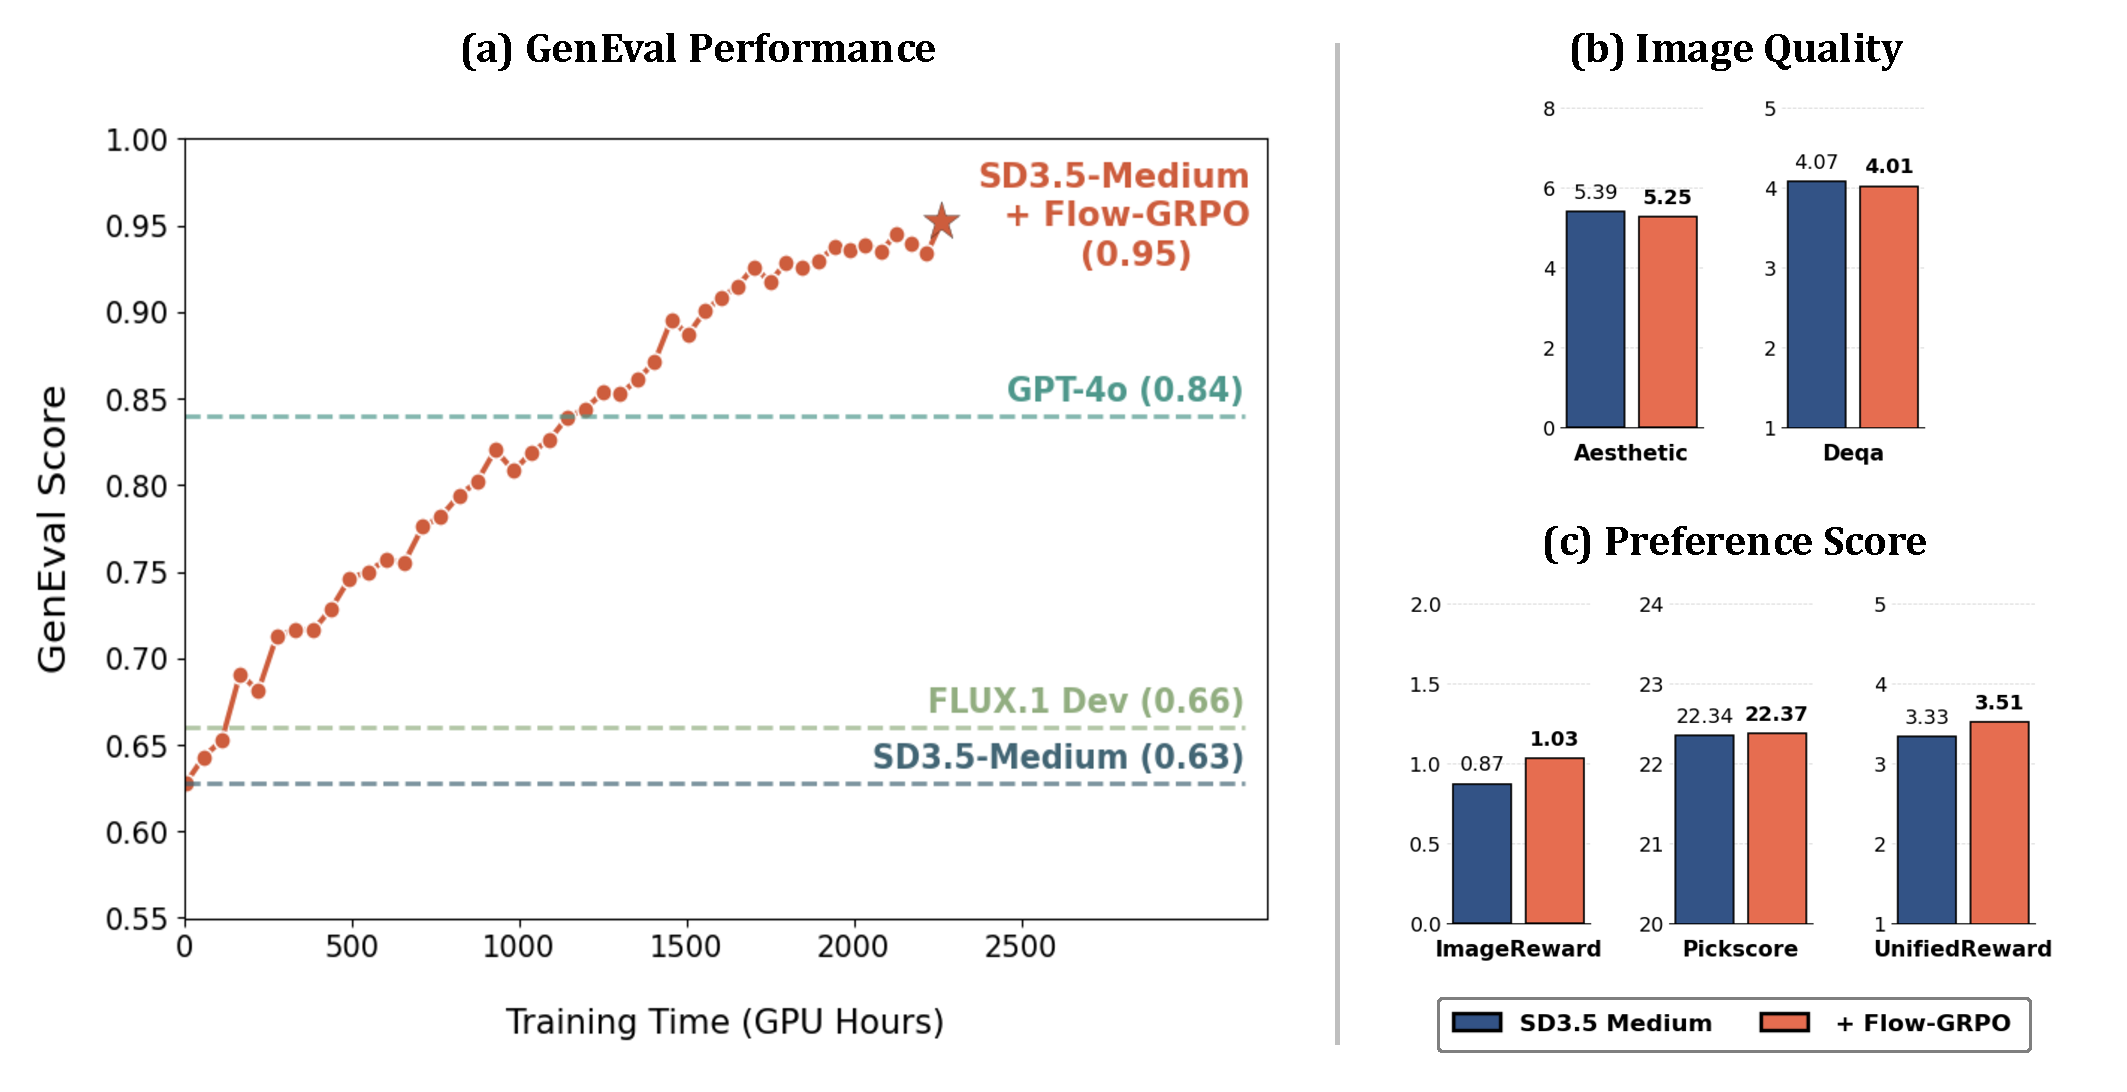
\includegraphics[width=\textwidth]{src/teaser.pdf}
\caption{ 
% \textcolor{pltred}{\textbf{(a) GenEval performance}} 
\textbf{(a) GenEval performance}
rises steadily throughout Flow-GRPO's training and outperforms GPT‑4o.
% \textcolor{pltgreen}{\textbf{(b) Image quality metrics}} 
\textbf{(b) Image quality metrics}
on DrawBench~\cite{drawbench} remain essentially unchanged.
% \textcolor{pltblue}{\textbf{(c) Human Preference Scores}} 
\textbf{(c) Human Preference Scores}
on DrawBench improves after training.
Results show that \emph{Flow-GRPO enhances the desired capability while preserving image quality and exhibiting minimal reward-hacking.}
}
\label{fig:teaser}
\vspace{-4mm}
\end{figure}
\section{Introduction}
\label{sec:intro}

Flow matching~\cite{lipman2022flow, rectified_flow} models have become dominant in image generation~\cite{sd3, flux2024} due to their solid theoretical foundations and strong performance in producing high quality images. However, they often struggle with composing complex scenes involving multiple objects, attributes, and relationships~\cite{T2i-compbench, Gpt-imgeval}, as well as text rendering~\cite{textdiffuser}. At the same time, online reinforcement learning (RL)~\cite{sutton1998reinforcement} has proven highly effective in enhancing the reasoning capabilities of large language models (LLMs)~\cite{deepseek_r1, openai_o1}. While previous research has mainly focused on applying RL to early diffusion-based generative models~\cite{ddpo} and offline RL techniques like direct preference optimization~\cite{dpo} for flow-based generative models~\cite{videoalign, skyreels_v2}, the potential of online RL in advancing flow matching generative models remains largely unexplored. In this study, we explore how online RL can be leveraged to effectively improve flow matching models.


Training flow models with RL presents several critical challenges: (1) Flow models rely on a deterministic generative process based on ODEs~\cite{rectified_flow}, meaning they cannot sample stochastically during inference. In contrast, RL relies on stochastic sampling to explore the environment, learning by trying different actions and improving based on rewards. \textit{This need for stochasticity in RL conflicts with the deterministic nature of flow matching models.} 
(2) Online RL depends on efficient sampling to collect training data, but flow models typically require many iterative steps to generate each sample, limiting efficiency. This issue is more pronounced with large models~\cite{flux2024, sd3}. To make RL practical for tasks like image or video generation, \textit{improving sampling efficiency is essential}.
% (2) {Online RL requires efficient sampling to gather training data, but flow models typically involve many iterative steps to generate each sample, significantly reducing sampling efficiency.} This issue becomes even more critical with large, advanced models~\cite{flux2024, sd3}, which are computationally intensive. Therefore, to make RL effective in tasks such as image or video generation, \textit{improving sampling efficiency within RL training is crucial}.

% (3) RL excels in improving LLM reasoning ability because mathematical tasks only require final-answer correctness. In contrast, image generation lacks a singular quality metric. For instance, in object counting tasks, optimizing solely for accurate object counts using the correctness of generated object counts as the reward model frequently results in correct quantities but reduced overall image quality.


% To address these challenges, 
% in this work, we propose the \textbf{Flow-GRPO} approach to introduce the GPRO~\cite{grpo} into the flow matching models for alignment on text-to-image tasks,
% where two key strategies are introduced.
% First, to overcome the deterministic limitations of the original flow model, we employ the \textbf{ODE-to-SDE} strategy by converting the ODE-based flow model into a Stochastic Differential Equation (SDE) framework. Specifically, in the ODE-to-SDE strategy, we convert the deterministic Flow-ODE into an equivalent Flow-SDE that matches the original model's marginal distributions, introducing randomness into the model's generation process.
% Second, to achieve high sampling efficiency for online RL, we introduce the \textbf{Denoise Reduction} strategy by reducing the denoising steps for training data generation while retaining the original denoising steps during inference.
% The key insight is that significant fewer denoising steps during RL training may be enough. In our experiemnts, we found training with fewer denoising steps matches the performance obtained with the full schedule while markedly cutting data‑generation cost.

To address these challenges, we propose \textbf{Flow-GRPO}, which integrates GRPO~\cite{grpo} into flow matching models for text-to-image (T2I) generation, using two key strategies.
First, we adopt the \textbf{ODE-to-SDE} strategy to overcome the deterministic nature of the original flow model. By converting the ODE-based flow into an equivalent Stochastic Differential Equation (SDE) framework, we introduce randomness while preserving the original marginal distributions.
Second, to improve sampling efficiency in online RL, we apply the \textbf{Denoising Reduction} strategy, which reduces denoising steps during training while keeping the full schedule during inference. Our experiments show that using fewer steps maintains performance while significantly reducing data generation costs.

% This reduction in computational complexity significantly accelerates the training process without compromising the model's performance. 
% Our experiments
 % Our method, in contrast, 
% , which aims to  stochastic sampling 
% (1) SDE sampling: By converting the ODE-based flow model into a Stochastic Differential Equation (SDE) framework, we enable stochastic sampling. This conversion introduces randomness into the model's generation process, overcoming the deterministic limitations of the original flow model. This approach is distinct from the traditional strategy in diffusion tasks, where the SDE is typically converted into an ODE to achieve higher generation quality.
% (2) FastDenoise: We utilize significantly fewer denoising steps during both sample generation and training, while retaining the original denoising steps during inference. The key insight behind this reduction strategy is that training on fewer denoising steps can xxx. This reduction in computational complexity significantly accelerates the training process without compromising the model's performance. Our experiments verify this: fewer denoising steps during training yield results comparable to those achieved with larger denoising steps during training.
% (3) applying a KL constraint instead of a general human-preference reward model to effectively prevent noticeable declines in image quality.

% We empirically evaluate our Flow-GRPO on text-to-image tasks with various reward types. (1) Verifiable rewards, primarily using the GenEval~\cite{geneval} benchmark and visual text rendering task. For example, GenEval comprises compositional image generation tasks (e.g., generating specified object counts, colors, and spatial relationships), which can be automatically assessed via traditional detection methods. On GenEval, Flow-GRPO improves Stable Diffusion 3.5 Medium (SD3-M)~\cite{sd3}’s accuracy from 63\% to 95\% (Figure~\ref{fig:teaser}), surpassing the performance of the state-of-the-art GPT-4o~\cite{gpt4o} model. For the visual text rendering task, we improve SD3-M's accuracy from 56\% to 92\%, significantly enhancing the model’s ability to generate text. (2) Model-based rewards, such as human preference Pickscore~\cite{kirstain2023pick} reward, further demonstrate that our framework is task-independent, highlighting its generalizability and robustness. 
We evaluate Flow-GRPO on T2I tasks with various reward types. (1) Verifiable rewards, using the GenEval~\cite{geneval} benchmark and visual text rendering task. GenEval includes compositional image generation tasks (e.g., generating specific object counts, colors, and spatial relationships), which can be automatically assessed with object detection methods. Flow-GRPO improves the accuracy of Stable Diffusion 3.5 Medium (SD3.5-M)~\cite{sd3} from 63\% to 95\% on GenEval, outperforming the state-of-the-art GPT-4o~\cite{gpt4o} model. For visual text rendering, SD3.5-M’s accuracy increases from 59\% to 92\%, greatly enhancing its text generation ability. (2) Model-based rewards, such as the human preference Pickscore~\cite{kirstain2023pick} reward. These results show that our framework is task independent, demonstrating its generalizability and robustness. Importantly, all improvements are achieved with very little reward hacking, as demonstrated in Figure~\ref{fig:teaser}.

% To summarize, our contribution is summarized as follows:
% \begin{itemize} [leftmargin=15pt]
%   \item We are the first to introduce GRPO to flow matching models by converting ODE sampling into SDE sampling, demonstrating that online RL is highly effective for T2I tasks. Specifically, our Flow-GRPO improves SD3-M accuracy from 63\% to 95\% without compromising image quality.
%   \item We find that for online RL, it is not necessary to use the standard longer timesteps when collecting training samples. We can utilize significantly fewer denoising steps during sample generation, while retaining the original denoising steps during testing, which can significantly accelerate the training process.
%   \item We demonstrate that the Kullback-Leibler (KL)  constraint is highly effective in preventing reward hacking\footnote{The reward becomes large, but image quality significantly decreases} without sacrificing image quality in image generation. 
%   We also note that KL is not simply analogous to early stopping. By adding an appropriate KL, we can achieve the same high reward as the KL-free version, , just with longer training time.
% \end{itemize}

To summarize, the contributions of Flow-GRPO are as follows:
\begin{itemize}[leftmargin=15pt]
\item We are the first to introduce GRPO to flow matching models by converting deterministic ODE sampling into SDE sampling, showing the effectiveness of online RL for T2I tasks. Flow-GRPO improves SD3.5-M accuracy from 63\% to 95\% without noticeably compromising image quality.
\item We find that online RL for flow matching models does not require the standard long timesteps for training sample collection. By using fewer denoising steps during training and retaining the original steps during testing, we can significantly accelerate the training process.
% \item We find that online RL with flow matching models can generate training samples with fewer denoising steps, greatly accelerating training. Full denoising is used at test time to maintain performance.
\item We show that the Kullback-Leibler (KL) constraint effectively prevents reward hacking, where reward increases at the cost of image quality or diversity. KL regularization is not empirically equivalent to early stopping. With a proper KL term, we can match the high reward of the KL-free version while preserving image quality, albeit with longer training.
\end{itemize}

\section{Related Work}

\paragraph{RL for LLM.} 
Online RL has effectively improved the reasoning abilities of LLMs, such as DeepSeek‑R1~\cite{deepseek_r1} and OpenAI‑o1~\cite{openai_o1}, using policy gradient methods like PPO~\cite{ppo} or value-free GRPO~\cite{grpo}. GRPO is more memory efficient by removing the need for a value network, so we adopt it in this work. PPO can also be applied to flow matching in a similar way.
\vspace{-2mm}
\paragraph{Diffusion and Flow Matching.}
Diffusion models~\cite{ho2020denoising, ddim, song2020score} add Gaussian noise to data and train a neural network to reverse the process. Sampling uses discrete DDPM steps or probability flow SDE solvers to generate high-fidelity outputs.
Flow matching~\cite{lipman2022flow, rectified_flow} learns a continuous-time normalizing flow by directly matching the velocity field, allowing efficient deterministic sampling with only a few ODE steps. It achieves competitive FID with far fewer denoising steps than diffusion, making it the dominant choice in recent image~\cite{sd3, flux2024} and video~\cite{kling, wanx, sora, hunyuanvideo} generation models.
Recent work~\cite{albergo2023stochastic, domingo2024adjoint} unifies diffusion and flow models under an SDE/ODE framework. Our work builds on their theoretical foundations and introduces GRPO to flow-based models.
\vspace{-2mm}
\paragraph{Alignment for T2I.}
Recent efforts to align pretrained T2I models with human preferences follow five main directions:
(1) direct fine-tuning with differentiable rewards~\cite{prabhudesai2023aligning, clark2023directly, xu2024imagereward, prabhudesai2024video};
(2) Reward Weighted Regression (RWR)~\cite{peng2019advantage, fan2025online, lee2023aligning,dong2023raft};
(3) Direct Preference Optimization (DPO) and variants~\cite{rafailov2024direct, wallace2024diffusion, videoalign, yang2024using, liang2024step, yuan2024self, liu2024videodpo, zhang2024onlinevpo, furuta2024improving,liang2025aesthetic};
(4) PPO-style policy gradients~\cite{schulman2017proximal, black2023training, fan2024reinforcement, gupta2025simple, miao2024training, zhao2025score};
(5) training-free alignment methods~\cite{yeh2024training, tang2024tuning, song2023loss}.
These methods have successfully aligned T2I models with human preferences, improving aesthetics and semantic consistency. Building on this progress, we introduce GRPO for flow matching models, the backbone of today's state-of-the-art T2I systems.
Concurrent work \cite{sun2025f5r} applies GRPO to text-to-speech flow models, but instead of converting the ODE to an SDE to inject stochasticity, they reformulate velocity prediction by estimating a Gaussian distribution (predicting both the mean and variance of
velocity), which requires retraining the pre-trained model. Another study~\cite{kim2025inference} also explores SDE-based stochasticity but focuses on inference-time scaling.


% \todo{This approach is distinct from the traditional strategy in diffusion tasks, where the SDE is typically converted into an ODE to achieve higher generation quality.}
% Framing alignment as a test-time search to maximize a reward function is not a novel formulation. However, most existing works either simplify autoregressive decoding as a bandit problem~\citep{gao2023scaling, beirami2024theoretical}, which limits their steerability, or require a value function learned from scratch to handle sparse preference rewards and prune search space~\citep{mudgal2023controlled, liu2023making}, which can be as difficult as training a large language model from scratch.
% Our work avoids these issues by parametrizing the sparse preference reward function with the log-probability difference between small tuned and untuned language models~\citep{rafailov2024direct}. This parametrization not only simplifies the search objective, allowing a simple greedy search algorithm to generate good results, but also reuses off-the-shelf models as steering forces, eliminating the need to train a reward or critic model from scratch.

% Concurrently with our work, Rafailov et al.~\citep{rafailov2024r} proposes a token-level MDP interpretation for language model alignment, demonstrating that a greedy probability search over a trained language model can achieve improvements over regular decoding. Our work builds on their theoretical foundations and proposes a practical greedy search algorithm designed for weak-to-strong guidance.
% % , i.e.,  conducting the probability search on the smaller models while sampling from the large model, in order to improve the generation quality of the large language model. 

% The idea of using small language models to align large language models has arisen in many recent works.
% The most related is proxy or emulated fine-tuning~\citep{liu2021dexperts, liu2024tuning, mitchell2023emulator, zhou2024emulated}, which uses the distributional difference of a small tuned and untuned model pair to modify the output distribution of a large model, approximating the output of the directly tuned large model. 
% However, these methods require that both small and large models share the same vocabulary, limiting their practical applications.
% In contrast, our approach does not modify the sampling distribution of the large model at the token level. Instead, we perform a tree search that periodically prioritizes the most promising states for further expansion (as evaluated by the small models) while sampling from the frozen large model's distribution. 
% Thus our approach does not require shared vocabulary and is applicable to black-box language models.



\section{Preliminaries}\label{sec:preliminaries}

In this section, we introduce the mathematical formulation of flow matching and describe how the denoising process can be mapped as a multi-step MDP.


\paragraph{Flow Matching.}\label{subsec:flow_matching}
Let \(\vx_0 \sim X_0\) be a data sample from the true distribution, and \(\vx_1 \sim X_1\) denote a noise sample. Recent advanced image-generation models (e.g., \cite{sd3,flux2024}) and video-generation models (e.g., \cite{kling,sora,wanx,hunyuanvideo}) adopt the Rectified Flow~\cite{rectified_flow} framework, which defines the “noised” data \(\vx_t\) as
\begin{equation}
\label{eq:flow_forward}
    \vx_t = (1-t)\,\vx_0 \;+\; t\,\vx_1,
\end{equation}
for \(t \in [0,1]\). Then a transformer model are trained to directly regress the velocity field \(\vv_\theta(\vx_t, t)\) by minimizing the Flow Matching objective \cite{lipman2022flow,rectified_flow}:
\begin{equation}
\label{eq:flow_loss}
    \loss(\theta) = \mathbb{E}_{t,\;\vx_0\sim X_0,\;\vx_1 \sim X_1} 
    \bigl[\;\|\vv \;-\; \vv_\theta(\vx_t,t)\|^2\bigr],
\end{equation}
where the target velocity field is \(\vv = \vx_1 - \vx_0\).

% The alignment of language models is typically cast as a KL-constrained optimization problem~\citep{ziegler2019fine}:
% \begin{subequations}
% \label{eq:obj}
% \begin{align}
%     \argmax_{\pi} \quad & \mathbb{E}_{\rvx \sim p(\rvx), \rvy \sim \pi(\rvy \mid \rvx)}\left[r(\rvx, \rvy)\right] \\
%     \text{s.t.} \quad & \mathbb{E}_{\rvx \sim p(\rvx)} \left[\mathbb{D}_{\mathrm{KL}}\left(\pi(\rvy \mid \rvx) \,\|\, \pi_{\mathrm{ref}}(\rvy \mid \rvx)\right)\right] \leq \epsilon,
% \end{align}
% \end{subequations}
% where $p(\rvx)$ is a distribution of prompts, $\rvy$ is the complete language model response, $r$ is a preference reward function that encourages human-preferred responses, and $\mathbb{D}_{\mathrm{KL}}$ limits how far the optimized language model $\pi$ can deviate from the reference (untuned) model $\pi_{\text{ref}}$.
% There are two main categories of alignment algorithms: (1) \textit{search-based} algorithms that optimize Eq.~\ref{eq:obj} with graph-based search during inference
% ~\citep{gao2023scaling, mudgal2023controlled, liu2023making, feng2023alphazero, mitchell2023emulator, liu2024tuning}, and (2) \textit{learning-based} algorithms that optimize Eq.~\ref{eq:obj} through gradient descent, aiming for a parametrized optimal language model~\citep{ziegler2019fine, zhao2023slic, rafailov2024direct, ethayarajh2024kto}. 
% Our work falls in the first category, proposing a search-based algorithm capable of using small language models to guide the decoding of a large language model to align with human preferences. 
% \footnote{For search-based algorithms, it is the response $\rvy$ that is searched rather than the language model $\pi$, therefore $\argmax_{\rvy}$ should be more appropriate. However, for brevity, we unify searching and learning in a unified framework ($\argmax_{\pi}$) by interpreting the searched responses as equivalently sampled from a latent model.}


\begin{figure}[t]
\centering
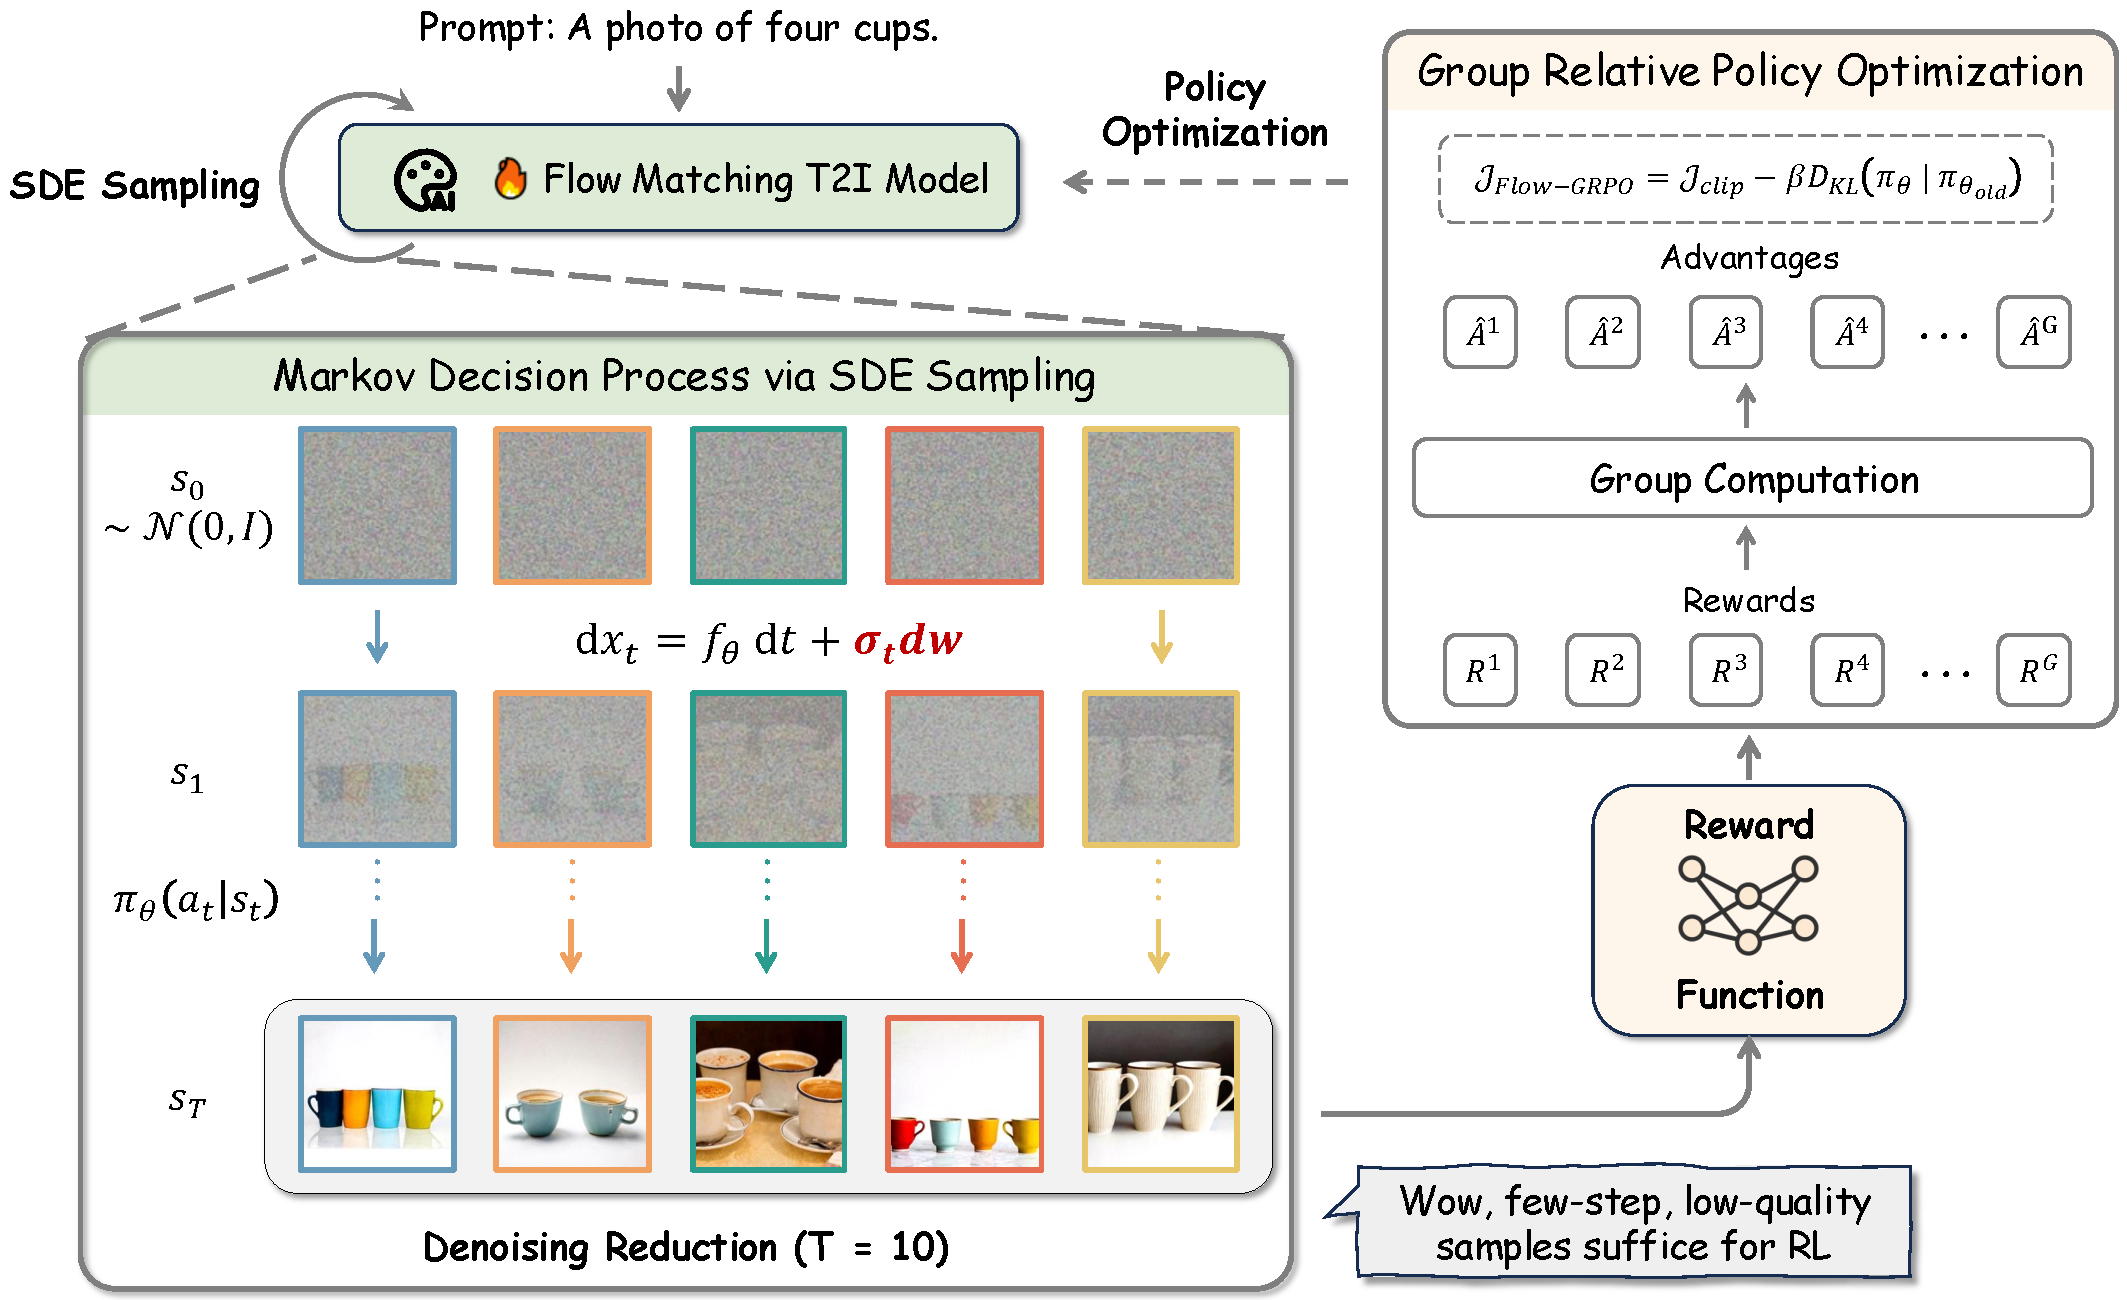
\includegraphics[width=0.9\textwidth]{src/method.pdf}
% \caption{Overview of Flow-GRPO. Given an input prompt, we first introduce the ODE-to-SDE strategy to implement stochastic sampling for online RL. Meanwhile, during the denoising process, we utilize the Denoising Reduction strategy to reduce the denoising steps in training to improve the sampling efficiency. Finally, we apply the GRPO strategy to perform the policy optimization and obtain the final aligned models.
% }
% \caption{Flow-GRPO processes an input prompt in three stages. First, an ODE-to-SDE strategy enables stochastic sampling for online RL. Second, a Denoising Reduction strategy reduces denoising steps during training to improve sampling efficiency. Finally, the GRPO strategy optimizes the policy to produce the aligned models.}
\caption{\textbf{Overview of Flow-GRPO.} 
Given a prompt set, we introduce an ODE-to-SDE strategy to enable stochastic sampling for online RL.
With Denoising Reduction (only T = 10 steps), we efficiently gather low-quality but still informative trajectories.
Rewards from these trajectories feed the GRPO loss, which updates the model online and yields an aligned policy.}
\vspace{-2mm}
\label{fig:method}
\end{figure}

\paragraph{Denoising as an MDP.}\label{subsec:denoising_as_mdp}
As shown in~\citep{ddpo}, the iterative denoising process in flow matching models can be formulated as a Markov Decision Process (MDP) \((\mathcal{S}, \mathcal{A}, \rho_0, P, R)\). The state at step \(t\) is \(\vs_t \triangleq (\vc, t, \vx_t)\), the action is the denoised sample \(\va_t \triangleq \vx_{t-1}\) predicted by the model, and the policy is \(\pi(\va_t \mid \vs_t) \triangleq p_\theta(\vx_{t-1} \mid \vx_t, \vc)\). 
The transition is deterministic: \(P(\vs_{t+1} \mid \vs_t, \va_t) \triangleq (\delta_\vc, \delta_{t-1}, \delta_{\vx_{t-1}})\), and the initial state distribution is \(\rho_0(\vs_0) \triangleq (p(\vc), \delta_T, \mathcal{N}(\mathbf{0}, \mathbf{I}))\), where \(\delta_y\) is the Dirac delta distribution centered at \(y\). 
The reward is only given at the final step: \(R(\vs_t, \va_t) \triangleq r(\vx_0, \vc)\) if \(t = 0\), and 0 otherwise.


% \begin{equation}
% \begin{aligned}
% \mathcal{J}_\text{GRPO}(\theta)& = \mathbb{E}_{(q,a)\sim \mathcal{D}, \{o_i\}_{i=1}^G\sim \pi_{\theta_\text{old}}(\cdot\mid q)} \\&
% \Bigg[ \frac{1}{G}\sum_{i=1}^{G} \frac{1}{|o_i|}\sum_{t=1}^{|o_i|} \Bigg( 
% \min \Big( r_{i,t}(\theta) \hat{A}_{i,t},  
% \ \text{clip} \Big( r_{i,t}(\theta), 1 - \varepsilon, 1 + \varepsilon \Big) \hat{A}_{i,t} \Big)
% - \beta D_{\text{KL}}(\pi_{\theta} || \pi_{\text{ref}}) 
% \Bigg) \Bigg],
% \label{eq:grpoloss}
% \end{aligned}
% \end{equation}
% where
% \begin{equation}
%     r_{i,t}(\theta)=\frac{\pi_{\theta}(o_{i,t} \mid q, o_{i,<t})}{\pi_{\theta_{\text{old}}}(o_{i,t} \mid q,o_{i,<t})}.
% \end{equation}

% The analytical solution to Eq.~\ref{eq:obj} can be obtained through the following Lagrangian~\citep{peng2019advantage, nair2020awac}:
% \begin{equation}\label{eq:lg-obj}
%     \mathcal{L(\pi, \beta)} = \mathbb{E}_{\rvx \sim p(\rvx), \rvy \sim \pi(\rvy \mid \rvx)}\left[r(\rvx, \rvy) + \beta\left(\epsilon - \mathbb{D}_{\mathrm{KL}}\left(\pi(\rvy \mid \rvx) \,\|\, \pi_{\mathrm{ref}}(\rvy \mid \rvx)\right)\right) \right],
% \end{equation}
% which has a well-known closed-form solution that expresses a duality between the reward function $r(\rvx, \rvy)$ and the optimal language model $\pi^*(\rvy \mid \rvx)$~\citep{ziebart2008maximum, levine2018reinforcement}:
% \begin{equation}\label{eq:duality}
%     r(\rvx, \rvy) = \beta \log \frac{\pi^*(\rvy \mid \rvx)}{\pi_{\text{ref}}(\rvy \mid \rvx)} + \beta \log Z(\rvx),
% \end{equation}
% where $Z(\rvx) = \sum_\rvy {\pi_{\text{ref}}(\rvy \mid \rvx)} \exp\left(\frac{1}{\beta}r(\rvx, \rvy)\right)$ denotes the partition function.
% One takeaway from this duality is that we can always express a reward function using tuned and untuned language models: (1) If a reward function is given~\citep{ziegler2019fine, stiennon2020learning, ouyang2022training}, we can first obtain the optimally tuned language model under this reward function with any learning-based algorithms, and then use the tuned and untuned models $(\pi^*, \pi_{\text{ref}})$ to reparametrize the reward function~\citep{lambert2024rewardbench}; (2) If a dataset is given from which the reward function can be derived, we can then directly parametrize the reward function with the tuned and untuned language models $(\pi^*, \pi_{\text{ref}})$ during reward modeling~\citep{rafailov2024direct}.
% so that the reward function and the optimal language model can be simultaneously obtained~\citep{rafailov2024direct}.
\input{sections/method}
\section{Experiments}\label{sec:exp}
This section empirically evaluates Flow-GRPO's ability to improve flow matching models on three tasks.
% First, in composition generation and text rendring,
% we use rule-based reward models to model the desired behaviors in each task and then  to steer larger models of various scales (Section~\ref{subsec:exp-geneval} \& Section~\ref{subsec:exp-text_rendering}).
% Next, xxx (Section~\ref{subsec:exp-instruction-following}).
(1) Composition Image Generation: This task requires precise object arrangement and attribute control. We report the results on GenEval. (2) Visual Text Rendering: a rule‑based task that evaluates the accurate rendering of the text specified in the prompt. (3) Human Preference Alignment: This task aims to align T2I models with human preferences.


\subsection{Experimental Setup}
\label{sec:exp_setup}
We introduce three tasks, detailing their respective prompts and reward definitions. For hyperparameter details and compute resource specifications, please refer to Appendix~\ref{app:subsubsec:synthetic-hyperp} and Appendix~\ref{app:subsubsec:synthetic-compute}.
% \paragraph{Baselines}
% Together with Flow-GRPO, we benchmark three established alignment methods, each implemented in its stronger online variant, since online updates typically yield better performance \cite{ddpo}.  
% At every training step we generate a group of images whose size matches that used by FlowPO, then apply one of the following update rules:
% \begin{itemize}
% \setlength{\itemindent}{-2em}
%   \item \textbf{Online SFT.} From each batch we select the <prompt, image> pair with the highest reward and perform supervised fine-tuning on these samples.
%   \item \textbf{Online Flow-AWR}~\cite{videoalign,awr}. Flow-AWR align models with reward-weighted likelihood maximization. In the online version we compute a softmax over the rewards in the current group and use the resulting weights to update the model.
%   \item \textbf{Online Flow-DPO}~\cite{videoalign}. Flow-DPO is the flow-matching analogue of DPO. For each batch we select the highest-reward image as the \emph{chosen} sample and the lowest-reward image as the \emph{rejected} sample, then optimise the DPO objective with this pair.
% \end{itemize}


% \subsection{Geneval}\label{subsec:exp-geneval}

% \paragraph{Setup.}
% Geneval assesses a text-to-image model’s ability to handle complex compositional requests, such as object counting, spatial relations, and attribute binding, across six tasks of ascending difficulty.
% We adopt the official evaluation pipeline, which first detects each object’s bounding box and color, then infers pairwise spatial relations. 我们使用geneval提供的构造脚本来构造训练所用的prompt~\footnote{}, 我们进行了严格的测试集过滤，包括'a photo of A and B'和'a photo of B and A'被认为是相同的，也会从训练集中去除
% Rewards are rule-based as follows:
% \begin{itemize}
% \setlength{\itemindent}{-2em}
%   \item \textbf{Counting:} \( r = |N_{\text{generation}} - N_{\text{prompt}}|\, / \,N_{\text{prompt}} \).
%   \item \textbf{Position / Color:} If the object count is correct, we assign a partial reward; the remainder is granted when the predicted position or color is also correct.
% \end{itemize}
% Therefore, the reward is bounded in the range \([0,1]\).


% \subsection{Text Rendering}\label{subsec:exp-text_rendering}
% \paragraph{Setup.}
% The prompt 格式是A sign that says 'Text to Image'. 引号里面是需要rendering的text. 我们使用gpt构造了20k的训练集和1k测试集
% Rewards are rule-based as \( r = |N_{\text{generation}} - N_{\text{prompt}}|\, / \,N_{\text{prompt}} \), where \((N_{\text{generation}}\) is the number of characters detected and \((N_{\text{prompt}}\)
%  is the number of prompt里被双引号包裹的字符
% **Task Selection:** We select three representative tasks:  
% - **Geneval:** A high-level task with rule-based dense rewards, requiring precise object arrangement and attribute control.  
% - **OCR: A high-level task with rule-based rewards, emphasizing text legibility and spatial accuracy.  
% - **Deqa:** A low-level task with VLM-based rewards, focusing on visual question-answering alignment.  
\paragraph{Compositional Image Generation.}\label{subsec:exp-geneval}
GenEval~\cite{geneval} assesses T2I models on complex compositional prompts—like object counting, spatial relations, and attribute binding—across six difficult compositional image generation tasks. We use its official evaluation pipeline, which detects object bounding boxes and colors, then infers their spatial relations. Training prompts are generated using official GenEval scripts, which apply templates and random combinations to construct the prompt dataset. The test set is strictly deduplicated: prompts differing only in object order (e.g., \texttt{"a photo of A and B"} vs. \texttt{"a photo of B and A"}) are treated as identical, and these variants are removed from the training set. Based on the base model's initial accuracy across the six tasks, we set the prompt ratio as \( \texttt{Position}:\texttt{Counting}:\texttt{Attribute Binding}:\texttt{Colors}:\texttt{Two Objects}:\texttt{Single Object} = 7:5:3:1:1:0\).
Rewards are rule-based: (1) \textbf{Counting:} \( r = 1-|N_{\text{gen}} - N_{\text{ref}}| / N_{\text{ref}} \); (2) \textbf{Position / Color:} If the object count is correct, a partial reward is assigned; the remainder is granted when the predicted position or color is also correct.

\paragraph{Visual Text Rendering~\cite{textdiffuser}.}\label{subsec:exp-text_rendering}
Text is common in images such as posters, book covers, and memes, so the ability to place accurate and coherent text inside the generated images is crucial for T2I models.
In our settings, we define an text rendering task, where each prompt follows the template \texttt{``A sign that says ``text''}.
Specifically,
the placeholder \texttt{``text''} is the exact string that should appear in the image.
We use GPT4o to produce 20K training prompts and 1K test prompts. Following \cite{seedream2}, we measure text fidelity with the reward
\(
r = \max (1-N_{\text{e}}/N_{\text{ref}}, 0),
\)
where \( N_{\text{e}} \) is the minimum edit distance
between the rendered text and the target text and \( N_{\text{ref}} \) is the number of characters inside the quotation marks in the prompt. This reward also serves as our metric of text accuracy.


\paragraph{Human Preference Alignment~\cite{kirstain2023pick}.} \label{subsec:exp-human_preference}
This task aims to align T2I models with human preferences. We use \texttt{PickScore}~\cite{kirstain2023pick} as our reward model, which is based on large-scale human annotated pairwise comparisons of images generated from the same prompt. For each image and prompt pair, \texttt{PickScore} provides an overall score that evaluates multiple criteria, such as the alignment of the image with the prompt and its visual quality.

\paragraph{Image Quality Evaluation Metric.}
% Because the T2I model is trained to maximise a predefined reward signal in RL, it is susceptible to reward hacking—situations in which the numerical reward rises but the quality or diversity of the generated images declines. This study aims to make online RL truly effective for T2I generation without compromising quality or diversity. To detect potential reward hacking beyond task-specific accuracy, we evaluate four automatic image quality metrics (i.e., Aesthetic score~\cite{schuhmann2022laion}, DeQA score~\cite{deqa}, ImageReward~\cite{xu2024imagereward}, UnifiedReward~\cite{wang2025unified}). See Appendix~\ref{app:subsubsec:quality_metric} for more details. Moreover, all metrics are evaluated on DrawBench~\cite{drawbench}, a comprehensive and challenging benchmark with diverse prompts for T2I models.
Since the T2I model is trained to maximize a predefined reward, it is vulnerable to reward hacking, where the reward increases but image quality or diversity declines. This study aims to make online RL effective for T2I generation without noticeably compromising quality or diversity. To detect reward hacking beyond task-specific accuracy, we evaluate four automatic image quality metrics: Aesthetic Score~\cite{schuhmann2022laion}, DeQA~\cite{deqa}, ImageReward~\cite{xu2024imagereward}, and UnifiedReward~\cite{wang2025unified} (see Appendix~\ref{app:subsubsec:quality_metric} for details). All metrics are computed on DrawBench~\cite{drawbench}, a comprehensive benchmark with diverse prompts for T2I models.
\begin{table*}[t]
    \centering
    \caption{{\bf GenEval Result.} 
Best scores are in \colorbox{pearDark!20}{blue}, second-best in \colorbox{color_green}{green}. Results for models other than SD3.5-M are from~\cite{Gpt-imgeval} or their original papers. Obj.: Object; Attr.: Attribution.}
    \resizebox{\linewidth}{!}{
    \begin{tabular}{l|c|cccccc}
    \toprule
    \textbf{Model} & \textbf{Overall} & \textbf{Single Obj.} & \textbf{Two Obj.} & \textbf{Counting} & \textbf{Colors} & \textbf{Position} & \textbf{Attr. Binding} \\
    \midrule
    \multicolumn{8}{c}{\textit{Diffusion Models}} \\
    \midrule
    LDM~\cite{rombach2022high}  & 0.37 & 0.92 & 0.29 & 0.23 & 0.70 & 0.02 & 0.05 \\
    SD1.5~\cite{rombach2022high}  & 0.43 & 0.97 & 0.38 & 0.35 & 0.76 & 0.04 & 0.06 \\
    SD2.1~\cite{rombach2022high}  & 0.50 & 0.98 & 0.51 & 0.44 & 0.85 & 0.07 & 0.17 \\
    SD-XL~\cite{podell2023sdxl}  & 0.55 & 0.98 & 0.74 & 0.39 & 0.85 & 0.15 & 0.23 \\
    DALLE-2~\cite{ramesh2022hierarchical}  & 0.52 & 0.94 & 0.66 & 0.49 & 0.77 & 0.10 & 0.19 \\
    DALLE-3~\cite{betker2023improving}  & 0.67 & 0.96 & 0.87 & 0.47 & 0.83 & 0.43 & 0.45 \\
    \midrule
    \multicolumn{8}{c}{\textit{Autoregressive Models}} \\
    \midrule
    % LlamaGen~\cite{sun2024autoregressive}  & 0.32 & 0.71 & 0.34 & 0.21 & 0.58 & 0.07 & 0.04 \\
    % Chameleon~\cite{team2024chameleon}  & 0.39 & - & - & - & - & - & - \\
    Show-o~\cite{xie2024show}  & 0.53 & 0.95 & 0.52 & 0.49 & 0.82 & 0.11 & 0.28 \\
    % LWM~\cite{liu2024world}  & 0.47 & 0.93 & 0.41 & 0.46 & 0.79 & 0.09 & 0.15 \\
    % SEED-X~\cite{ge2024seedx}  & 0.49 & 0.97 & 0.58 & 0.26 & 0.80 & 0.19 & 0.14 \\
    Emu3-Gen~\cite{wang2024emu3}  & 0.54 & 0.98 & 0.71 & 0.34 & 0.81 & 0.17 & 0.21 \\
    % TokenFlow-XL~\cite{qu2024tokenflow}  & 0.55 & 0.95 & 0.60 & 0.41 & 0.81 & 0.16 & 0.24 \\
    % Janus~\cite{wu2410janus}  & 0.61 & 0.97 & 0.68 & 0.30 & 0.84 & 0.46 & 0.42 \\
    JanusFlow~\cite{ma2024janusflow}  & 0.63 & 0.97 & 0.59 & 0.45 & 0.83 & 0.53 & 0.42 \\
    Janus-Pro-7B~\cite{chen2025janus}  & 0.80 & \colorbox{color_green}{0.99} & 0.89 & 0.59 & \colorbox{color_green}{0.90} & \colorbox{color_green}{0.79} & \colorbox{color_green}{0.66} \\
    % GoT~\cite{fang2025got}  & 0.64 & 0.99 & 0.69 & 0.67 & 0.85 & 0.34 & 0.27 \\
    % HiDream-I1  & 0.83 & \textbf{1.00} & \textbf{0.98} & 0.79 & 0.91 & 0.60 & \textbf{0.72} \\
    GPT-4o~\cite{gpt4o} & \colorbox{color_green}{0.84} & \colorbox{color_green}{0.99} & 0.92 & 0.85 & \colorbox{pearDark!20}{0.92} & 0.75 & 0.61 \\
    \midrule
    \multicolumn{8}{c}{\textit{Flow Matching Models}} \\
    \midrule
    FLUX.1 Dev~\cite{flux2024}  & 0.66 & 0.98 & 0.81 & 0.74 & 0.79 & 0.22 & 0.45 \\
    SD3.5-L~\cite{sd3}  & 0.71 & 0.98 & 0.89 & 0.73 & 0.83 & 0.34 & 0.47 \\
    SANA-1.5 4.8B~\cite{xie2025sana} & 0.81 & \colorbox{color_green}{0.99} & \colorbox{color_green}{0.93} & \colorbox{color_green}{0.86} & 0.84 & 0.59 & 0.65 \\
    SD3.5-M~\cite{sd3} & 0.63 & 0.98 & 0.78 & 0.50 & 0.81 & 0.24 & 0.52 \\
    \midrule
    \textbf{SD3.5-M+Flow-GRPO} & \colorbox{pearDark!20}{0.95} & \colorbox{pearDark!20}{1.00} & \colorbox{pearDark!20}{0.99} & \colorbox{pearDark!20}{0.95} & \colorbox{pearDark!20}{0.92} & \colorbox{pearDark!20}{0.99} & \colorbox{pearDark!20}{0.86}  \\
    \bottomrule
    \end{tabular}
    }
    \label{tab:geneval}
    \end{table*}
\definecolor{pltcount}{HTML}{2C424B}
\definecolor{pltcolor}{HTML}{7E946E}
\definecolor{pltpos}{HTML}{6D9992}
\definecolor{pltattr}{HTML}{9A4730}
\begin{figure}[t]
\centering
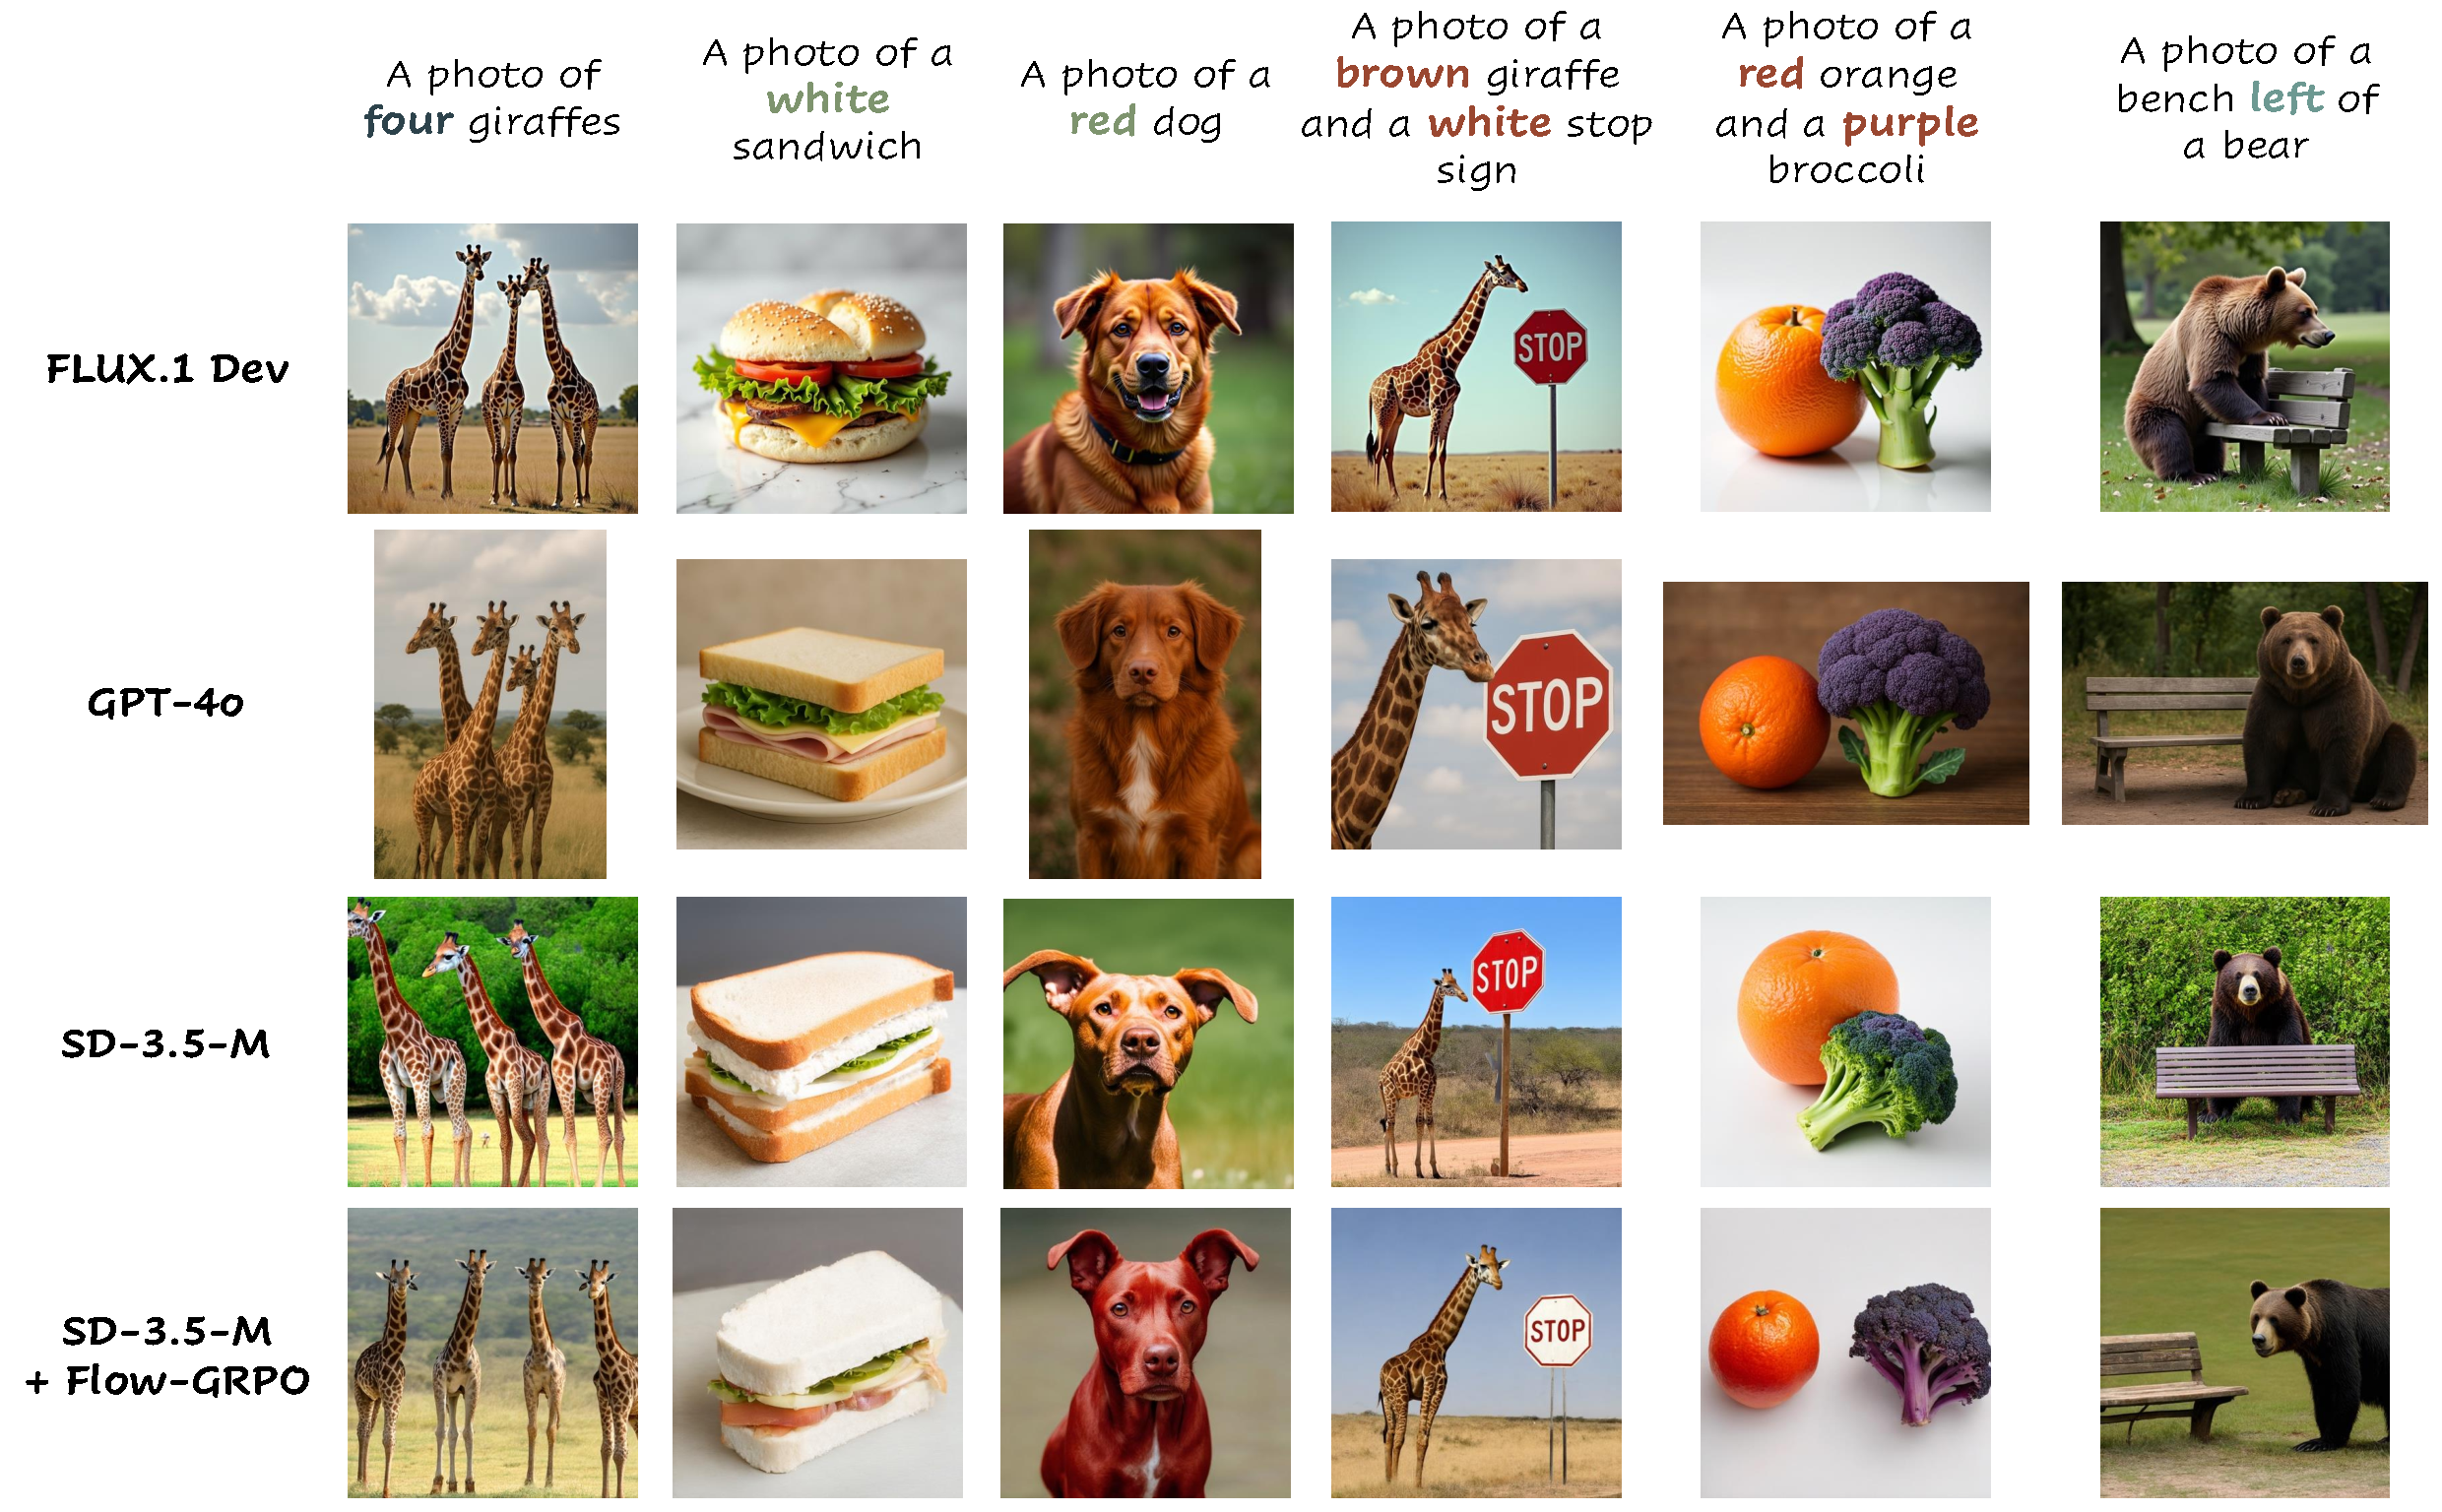
\includegraphics[width=\textwidth]{src/experiments/result_geneval.pdf}
\caption{\textbf{Qualitative Comparison on the GenEval Benchmark.} Our approach demonstrates superior performance in 
\textbf{\textcolor{pltcount}{Counting}}, 
\textbf{\textcolor{pltcolor}{Colors}}, 
\textbf{\textcolor{pltattr}{Attribute Binding},
and \textbf{\textcolor{pltpos}{Position}}}.
}
\vspace{-2mm}
\label{fig:result_geneval}
\end{figure}


\begin{table*}[t]
    \centering
    \renewcommand{\arraystretch}{1.1}
    \caption{\textbf{Performance on Compositional Image Generation, Visual Text Rendering, and Human Preference} benchmarks, evaluated by task performance on test prompts, and by image quality and preference scores on DrawBench prompts. ImgRwd: ImageReward; UniRwd: UnifiedReward.}
    \resizebox{\linewidth}{!}{
        \begin{tabular}{lcccccccc}
            \toprule
            \multirow{2}{*}{\textbf{Model}} & \multicolumn{3}{c}{\textbf{Task Metric}} & \multicolumn{2}{c}{\textbf{Image Quality}} & \multicolumn{3}{c}{\textbf{Preference Score}}    \\ \cmidrule(lr){2-4} \cmidrule(lr){5-6} \cmidrule(l){7-9} 
                                   & \textbf{GenEval}  & \textbf{OCR Acc.}  & \textbf{PickScore} & \textbf{Aesthetic}          & \textbf{DeQA}         & \textbf{ImgRwd} & \textbf{PickScore} & \textbf{UniRwd} \\ \midrule
            SD3.5-M & 0.63 & 0.59 & 21.72 & 5.39 & 4.07 & 0.87 & 22.34 & 3.33 \\
            \midrule
            % \addlinespace[3pt]
            % \rowcolor{gray!15}
            \multicolumn{9}{c}{\textit{Compositional Image Generation}} \\
            \midrule
            % \rowcolor{gray!05}
            Flow-GRPO (w/o KL) & 0.95 & — & — & 4.93 & 2.77 & 0.44 & 21.16 & 2.94 \\
            % \rowcolor{gray!05}
            \rowcolor{gray!20} Flow-GRPO (w/ KL)  & 0.95 & — & — & 5.25 & 4.01 & 1.03 & 22.37 & 3.51 \\

            \midrule
            % \addlinespace[3pt]
            % \rowcolor{gray!15}
            \multicolumn{9}{c}{\textit{Visual Text Rendering}} \\
            \midrule
            Flow-GRPO (w/o KL) & — & 0.93 & — & 5.13 & 3.66 & 0.58 & 21.79 & 3.15 \\
            \rowcolor{gray!20} Flow-GRPO (w/ KL)  & — & 0.92 & — & 5.32 & 4.06 & 0.95 & 22.44 & 3.42 \\
            
            \midrule
            % \rowcolor{gray!15}
            \multicolumn{9}{c}{\textit{Human Preference Alignment}} \\
            \midrule
            % \rowcolor{gray!05}
            Flow-GRPO (w/o KL) & — & — & 23.41 & 6.15 & 4.16 & 1.24 & 23.56 & 3.57 \\
            % \rowcolor{gray!05}
            \rowcolor{gray!20} Flow-GRPO (w/ KL)  & — & — & 23.31 & 5.92 & 4.22 & 1.28 & 23.53 & 3.66 \\
            \bottomrule
            \end{tabular}
}
\vspace{-2mm}
\label{tab:all_task}
\end{table*}


% \begin{figure}[htbp]
% \centering
% \includegraphics[width=0.9\textwidth]{src/experiments/compare_curve3.pdf}
% \caption{Comparison of Flow-GRPO and Other Alignment Methods on the Compositional Image Generation task. \todo
% }
% \label{app:fig:compare_curva_geneval}
% \end{figure}

\begin{figure}[htbp]
  \centering
  \begin{minipage}[t]{0.49\textwidth}
    \centering
    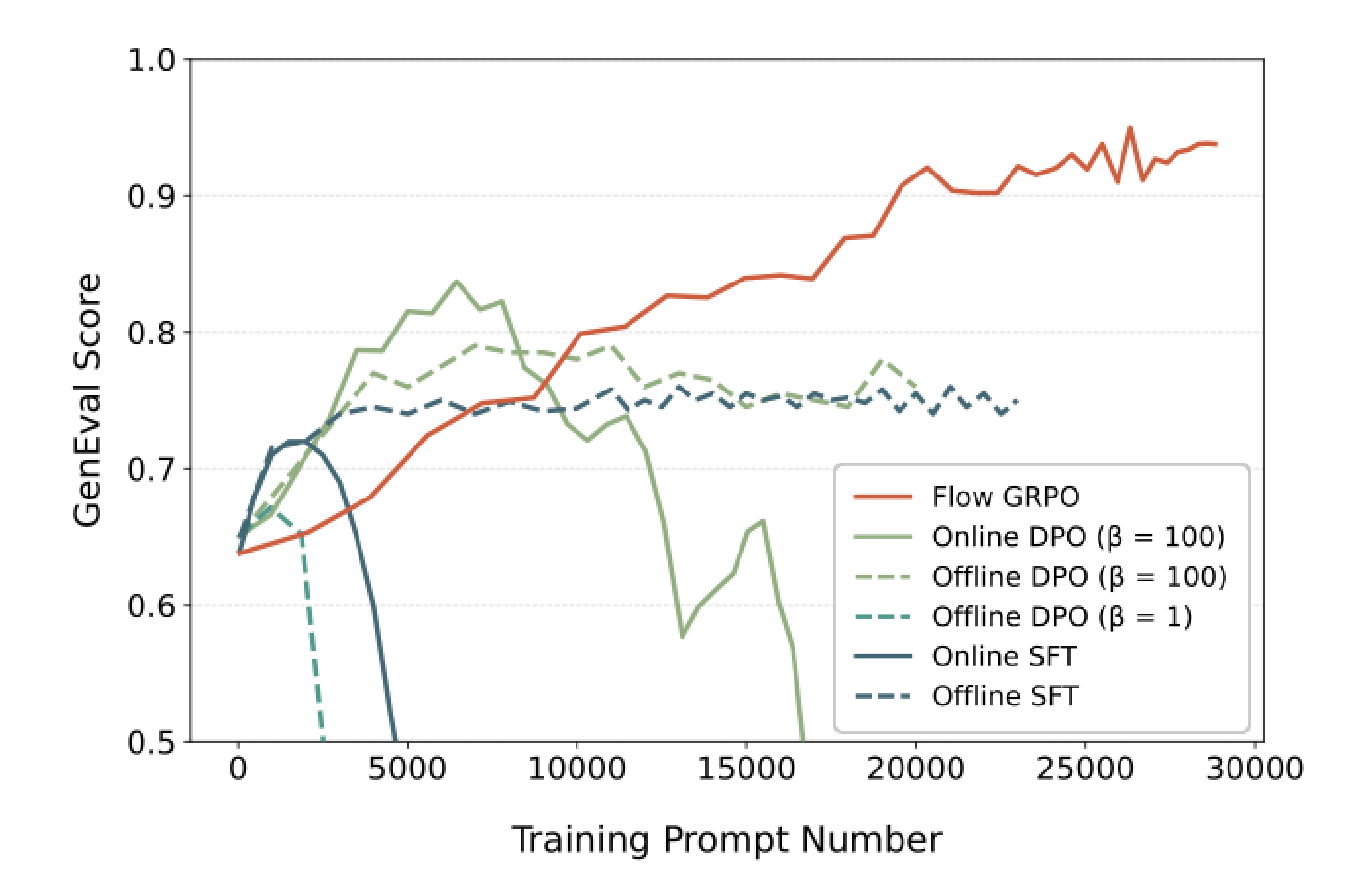
\includegraphics[width=\linewidth]{src/experiments/compare_curve_3.pdf}
    \vspace{-1.5em}
    \caption{
    Comparison with Other Alignment Methods on the Compositional Generation Task.
    % Comparison with Other Alignment Methods on the GenEval Task.
    }
    \label{app:fig:compare_curva_geneval}
  \end{minipage}
  \hfill
  \begin{minipage}[t]{0.47\textwidth}
    \centering
    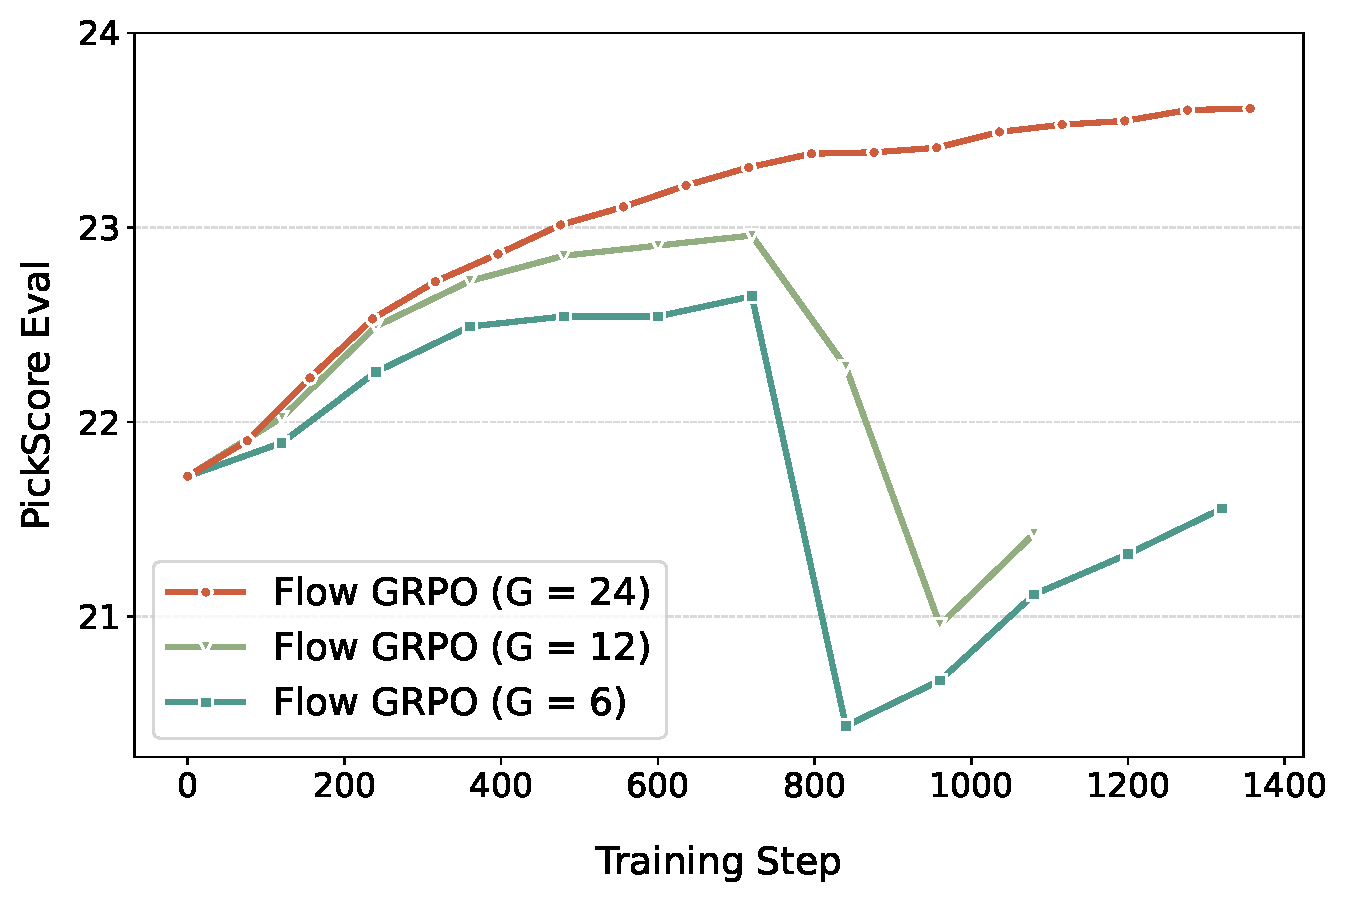
\includegraphics[width=\linewidth]{src/experiments/camera_ready_add/camera_ready_group.pdf}
    \vspace{-1.5em}
    \caption{Ablation Studies on Different Group Size $G$. Higher group size performs better.}
    \label{fig:abltion_groupsize}
  \end{minipage}
\end{figure}
% \paragraph{Results.} 

% **Experiments**  

\subsection{Main Results}  
Figure~\ref{fig:teaser} and Table~\ref{tab:geneval} show Flow-GRPO's GenEval performance steadily improving during training, ultimately outperforming GPT-4o. This occurs while maintaining both image quality metrics and preference scores on DrawBench, a benchmark with diverse and comprehensive prompts for evaluating general model capabilities. Figure~\ref{fig:result_geneval} offers qualitative comparisons.
Beyond Compositional Image Generation, Table~\ref{tab:all_task} details evaluations on Visual Text Rendering and Human Preference tasks. Flow-GRPO improved text rendering ability, again without decreasing image quality metrics and preference scores on DrawBench. 
See Figures~\ref{app:fig:add_qualitative_result_geneval}, \ref{app:fig:add_qualitative_result_ocr} \& \ref{app:fig:add_qualitative_result_pickscore} in Appendix~\ref{app:subsec:qualitative_results} for related qualitative examples.
For the Human Preference task, image quality did not decrease without KL regularization. However, we found that omitting KL caused a collapse in visual diversity, a form of reward hacking discussed further in Section~\ref{sec:subsec:reward_hacking}.
These results demonstrate that Flow-GRPO boosts desired capabilities while causing very little degradation to image quality or visual diversity.

% We also compare Flow-GRPO with other alignment methods, including supervised fine-tuning, reward weighted regression~\cite{videoalign, awr}, Flow-DPO~\cite{videoalign}, and their online variants. Flow-GRPO outperforms all of them by a large margin. See Appendix~\ref{app:subsec:baselines} for details.
\paragraph{Flow-GRPO vs. Other Alignment Methods.}
We compare Flow-GRPO with several alignment methods: supervised fine-tuning (SFT), Flow-DPO~\cite{videoalign,wallace2024diffusion}, and their online variants. Flow-GRPO consistently outperforms all baselines by a significant margin.
At each step, we generate a group of images using the same group size as in Flow-GRPO. The only difference lies in the update rule:
\begin{itemize}
\setlength{\itemindent}{-2em}
\item \textbf{SFT}: Select the highest-reward image in each group and fine-tune on it.
\item \textbf{Flow-DPO}: Use the highest-reward image in each group as the chosen sample and the lowest as the rejected, then apply the DPO loss.
\end{itemize}

Offline variants use a fixed pretrained model for data collection, while online variants update their data collection models every 40 steps. As shown in Figure~\ref{app:fig:compare_curva_geneval}, Flow-GRPO outperforms all baselines. Online DPO also surpasses its offline counterpart, consistent with~\cite{skyreels_v2}. For the second-best online DPO, a hyperparameter search on its key parameter $\beta$ revealed that smaller values are not always optimal; excessively small $\beta$ values can cause training collapse. Appendix~\ref{app:sec:extened-exp-results} presents more comprehensive comparisons covering additional methods and tasks.

% \begin{table}[ht]
% \centering
% \begin{tabular}{l|lccccccc}
% \toprule
% % \multirow{2}{*}
% {\textbf{Type}} & {\textbf{Method}} &  \textbf{Single Obj.} & \textbf{Two Obj.} & \textbf{Counting} & \textbf{Colors} & \textbf{Position} & \textbf{Color Attr.} & \textbf{Overall} \\ 
% \midrule

% \multirow{6}{*}{\textbf{Diffusion Only}} 
% & SDXL [88] & 98 & 74 & 39 & 85 & 15 & 23 & 55 \\ 
% & FLUX.1-dev [57] & 98 & 79 & 73 & 77 & 22 & 45 & 66 \\ 
% & DALL-E 3 [100] & 96 & 87 & 47 & 83 & 43 & 45 & 67 \\ 
% & SD3-Medium [24] & 99 & 94 & 72 & 89 & 33 & 60 & 74 \\ 
% & CogView4-6B [3] & 99 & 86 & 66 & 79 & 48 & 58 & 73 \\ 
% \midrule

% \multirow{5}{*}{\textbf{Hybrid Model}} 
% & SEED-X [29] & 97 & 58 & 26 & 80 & 19 & 14 & 49 \\ 
% & Transfusion [133] & - & - & - & - & - & - & 63 \\
% & D-DiT [64] & 97 & 80 & 54 & 76 & 32 & 50 & 65 \\ 
% & Show-o [124] & 98 & 80 & 66 & 84 & 31 & 50 & 68 \\ 
% & GPT-4ot [81] & 99 & 92 & 85 & 91 & 75 & 66 & 85 \\
% % \hline
% \bottomrule
% \end{tabular}
% \caption{Performance comparison of different methods across metrics.}
% \label{tab:comparison}
% \end{table}

% \begin{table}[ht]
% \centering
% \caption{Performance comparison of different methods across metrics. ``Single Obj.'', ``Two Obj.'', ``Pos.'' and ``Attr. binding'' denote ``Single Object'', ``Two Object'', ``Position'' and ``Attribute binding'', respectively.}

% \begin{tabular}{l|ccccccc}
% \toprule
% % \multirow{2}{*}
%  {\textbf{Method}} &  \textbf{Single Obj.} & \textbf{Two Obj.} & \textbf{Counting} & \textbf{Colors} & \textbf{Pos.} & \textbf{Attr. binding} & \textbf{Overall} \\ 
% \midrule
% \multicolumn{8}{c}{\textit{Diffusion Only}} \\
% \midrule

% SDXL & 98 & 74 & 39 & 85 & 15 & 23 & 55 \\ 
% FLUX.1-dev  & 98 & 79 & 73 & 77 & 22 & 45 & 66 \\ 
% DALL-E3 & 96 & 87 & 47 & 83 & 43 & 45 & 67 \\ 
% SD3-Medium & 99 & 94 & 72 & 89 & 33 & 60 & 74 \\ 
% CogView4-6B & 99 & 86 & 66 & 79 & 48 & 58 & 73 \\ 
% \midrule
% \multicolumn{8}{c}{\textit{Hybrid Model}} \\
% \midrule
% % \multirow{5}{*}{\textbf{Hybrid Model}} 
% SEED-X & 97 & 58 & 26 & 80 & 19 & 14 & 49 \\ 
% Transfusion & - & - & - & - & - & - & 63 \\
% D-DiT& 97 & 80 & 54 & 76 & 32 & 50 & 65 \\ 
% Show-o & 98 & 80 & 66 & 84 & 31 & 50 & 68 \\ 
% GPT-4o & 99 & 92 & 85 & 91 & 75 & 66 & 85 \\
% % \hline
% \bottomrule
% \end{tabular}
% \label{tab:comparison}
% \end{table}

% **Implementation Details:** All experiments use Stable Diffusion 3 (SD3) with LoRA fine-tuning (rank=32) and timestep fraction scheduling. Training runs on 24–32 GPUs with KL regularization (β=0.004–0.04) unless specified.  


% \begin{figure}[t]
% \centering
% 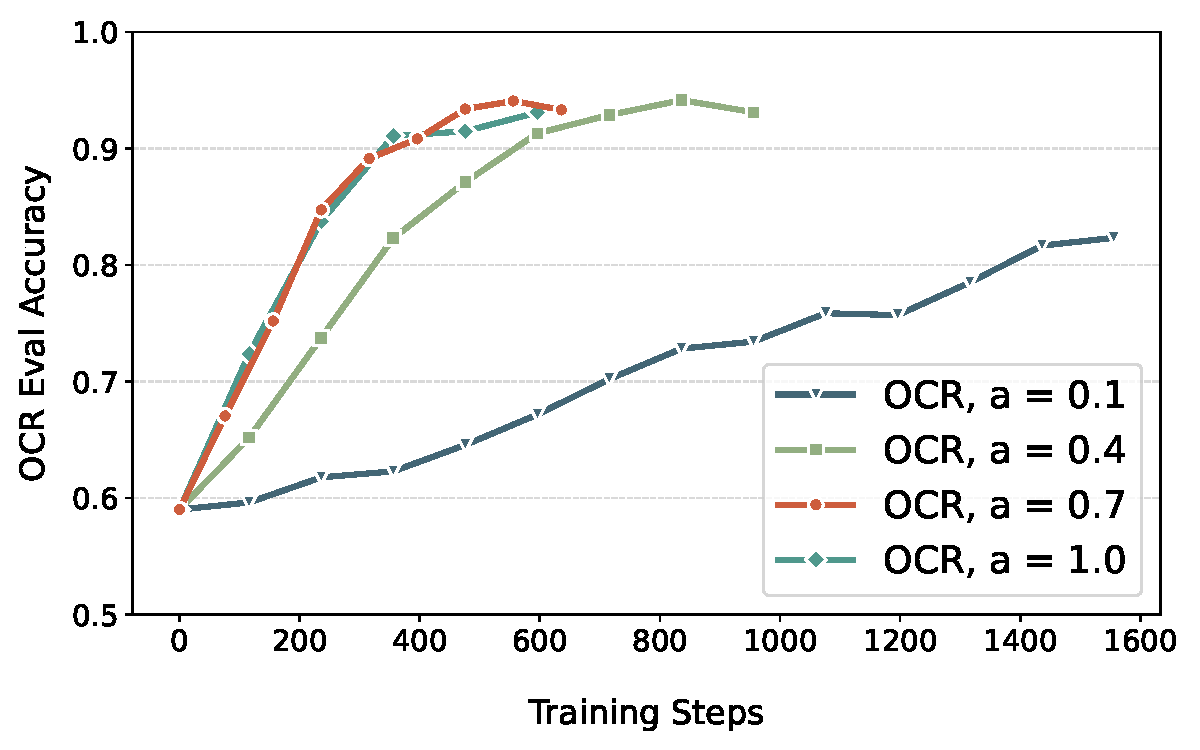
\includegraphics[width=0.5\textwidth]{src/experiments/ablation_noise/exp1_ocr_ablation_noise.pdf}
% \caption{Increasing the noise level $a$ boosts exploration and speeds up training.
% }
% \label{fig:exp1_ocr_ablation_noise}
% \end{figure}

% \begin{figure}[htbp]
%   \centering
%   \begin{minipage}[t]{0.48\textwidth}
%     \centering
%     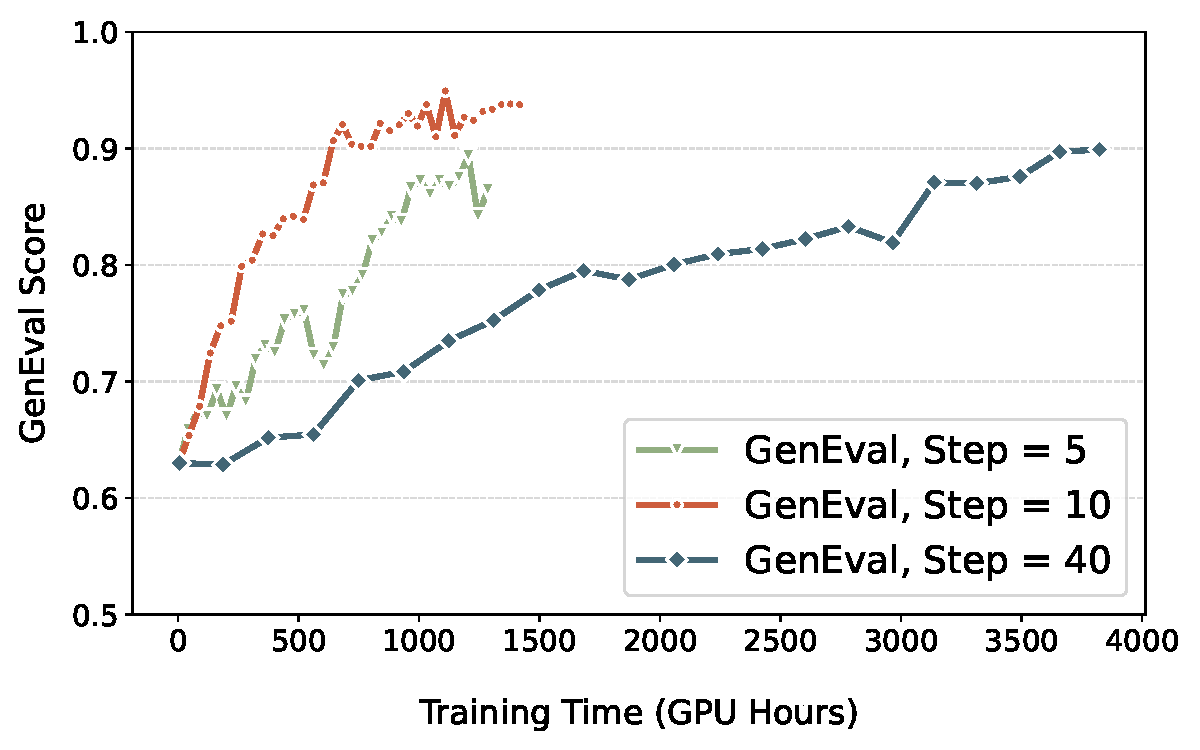
\includegraphics[width=\linewidth]{src/experiments/ablation_step/exp2_geneval_ablation_step.pdf}
%     \vspace{-1.5em}
%     \caption*{\footnotesize (a). Experiments on GenEval}
%   \end{minipage}
%   \hfill
%   \begin{minipage}[t]{0.48\textwidth}
%     \centering
%     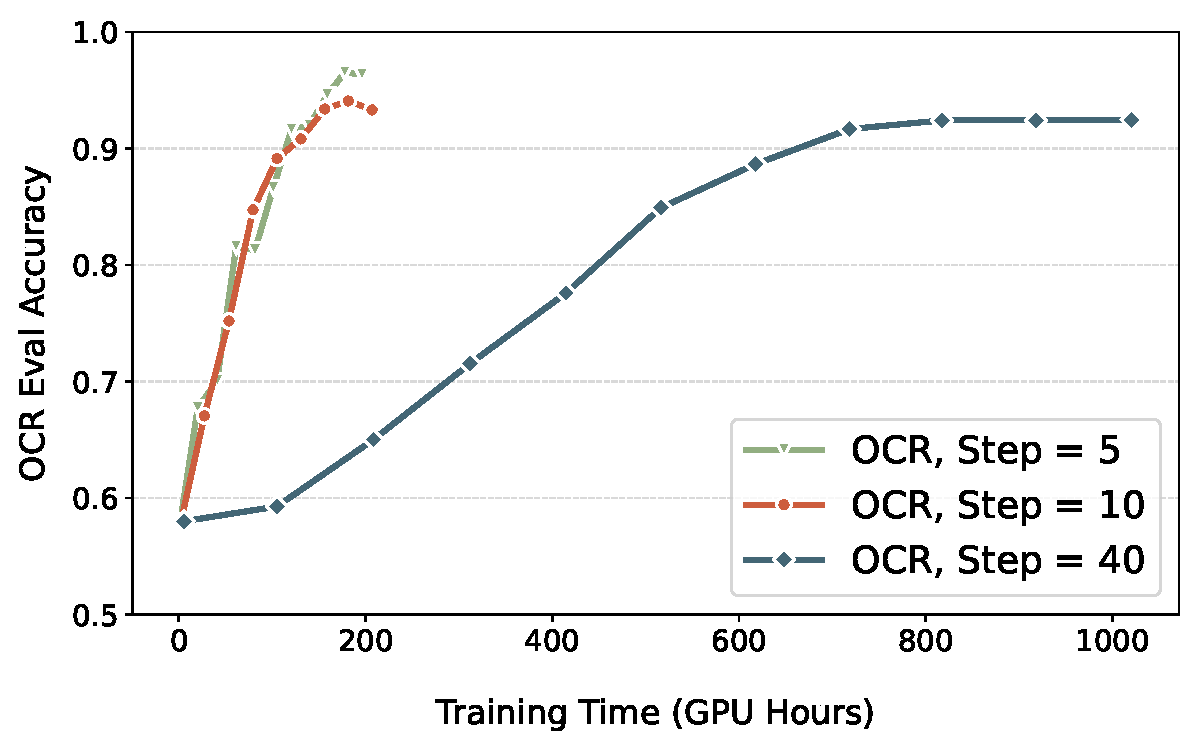
\includegraphics[width=\linewidth]{src/experiments/ablation_step/exp2_ocr_ablation_step.pdf}
%     \vspace{-1.5em}
%     \caption*{\footnotesize (b).  Experiments on OCR}
%   \end{minipage}
%   \vspace{1.5em}

%   \begin{minipage}[t]{0.48\textwidth}
%     \centering
%     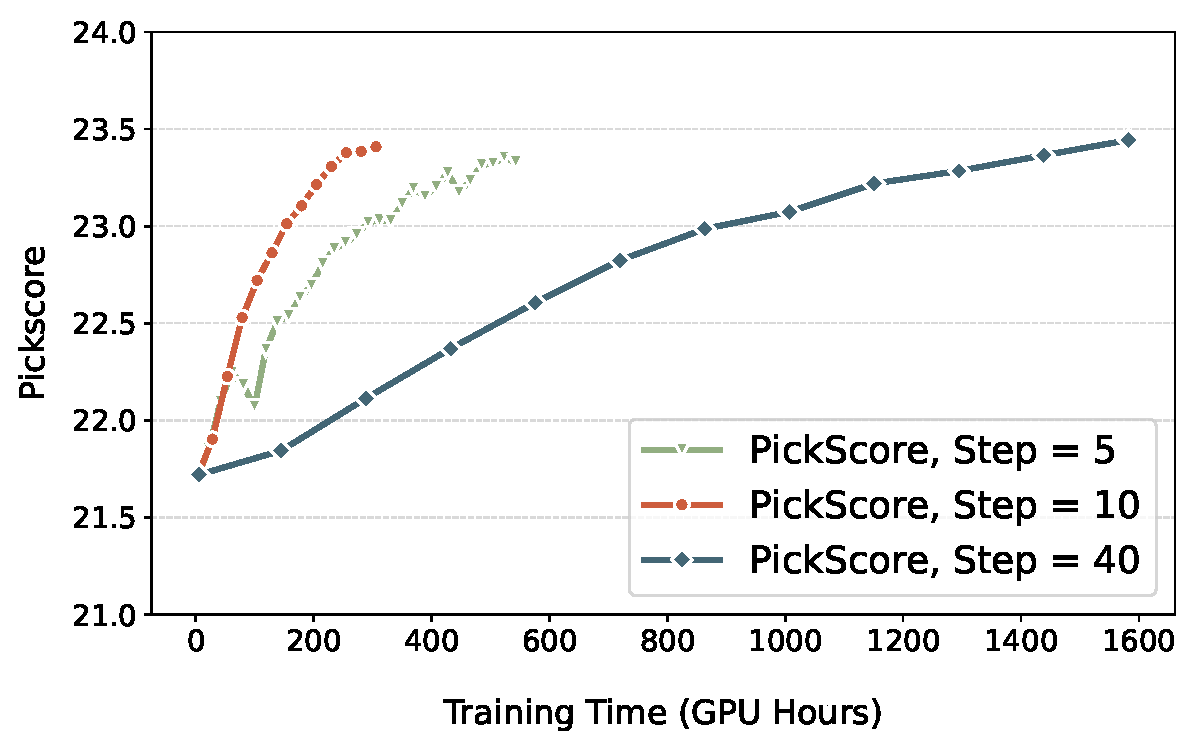
\includegraphics[width=\linewidth]{src/experiments/ablation_step/exp2_pickscore_ablation_step.pdf}
%     \vspace{-1.5em}
%     \caption*{\footnotesize (c). Experiments on PickScore}
%   \end{minipage}

%   \caption{To be added}
%   \label{fig:exp2_ablation_step}
% \end{figure}


% \begin{figure}[htbp]
%   \centering
%   \begin{minipage}[t]{0.48\textwidth}
%     \centering
%     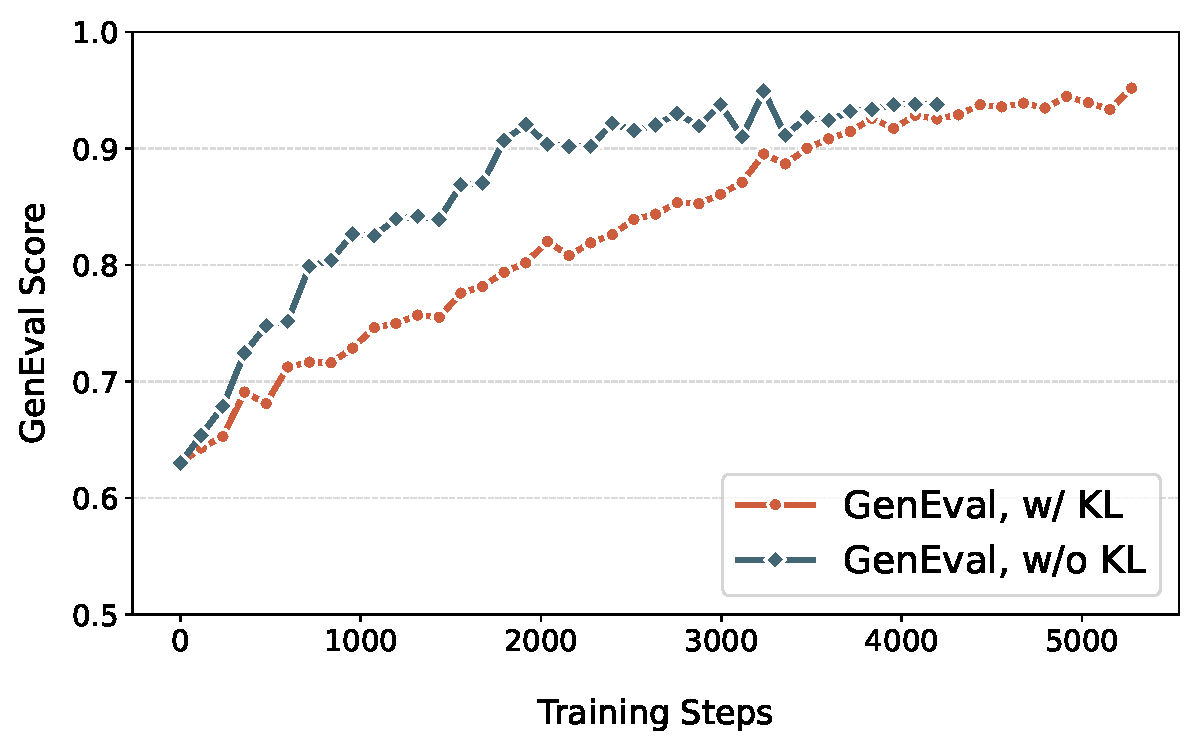
\includegraphics[width=\linewidth]{src/experiments/ablation_kl/exp3_geneval_ablation_kl.pdf}
%     \vspace{-1.5em}
%     \caption*{\footnotesize (a). Experiments on GenEval}
%   \end{minipage}
%   \hfill
%   \begin{minipage}[t]{0.48\textwidth}
%     \centering
%     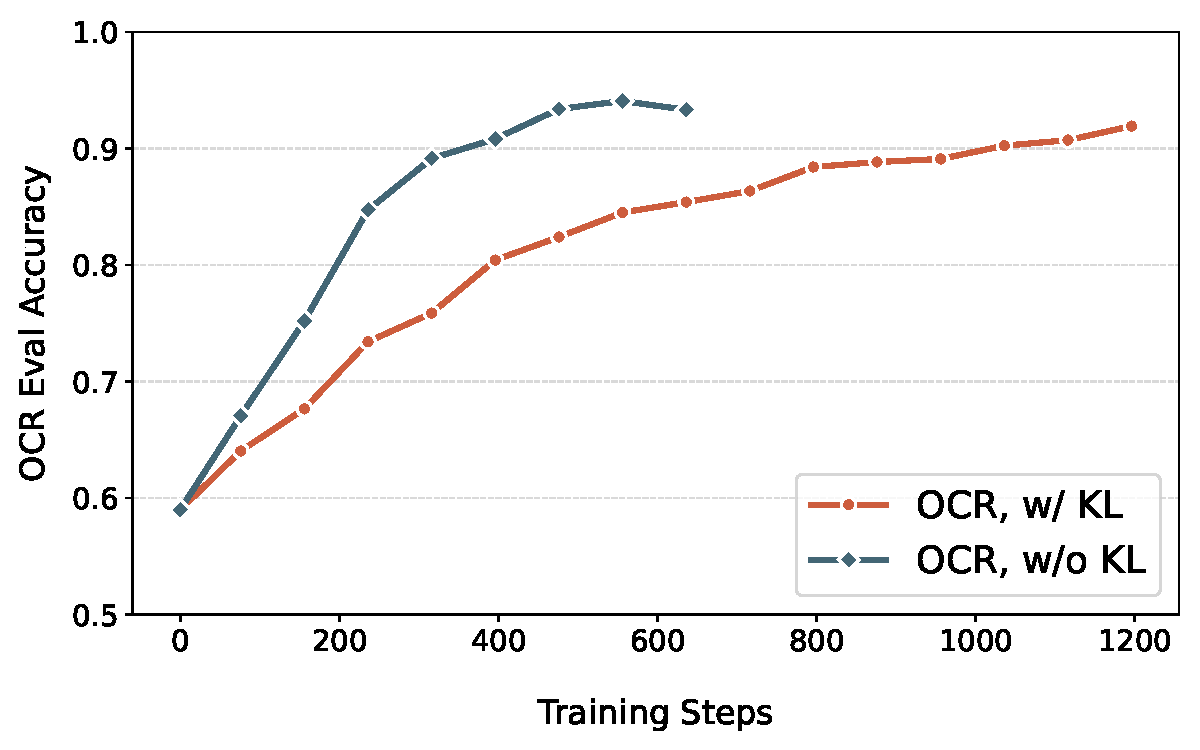
\includegraphics[width=\linewidth]{src/experiments/ablation_kl/exp3_ocr_ablation_kl.pdf}
%     \vspace{-1.5em}
%     \caption*{\footnotesize (b).  Experiments on OCR}
%   \end{minipage}
%   \vspace{1.5em}

%   \begin{minipage}[t]{0.48\textwidth}
%     \centering
%     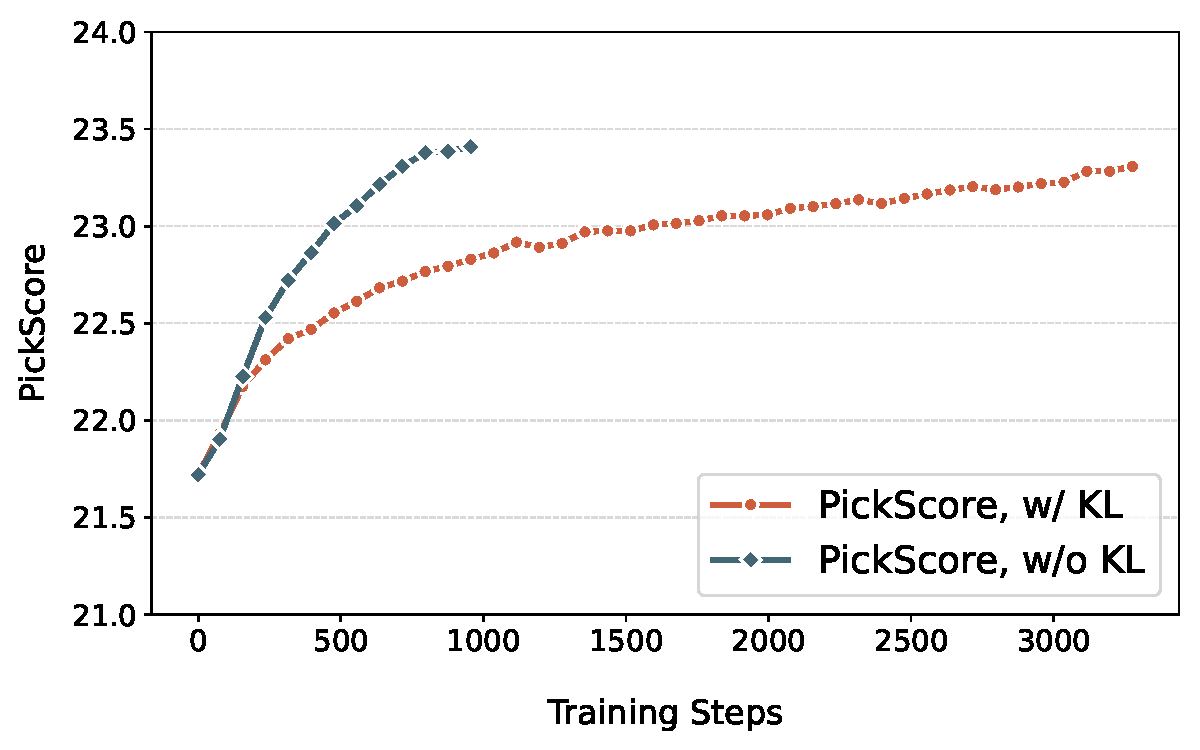
\includegraphics[width=\linewidth]{src/experiments/ablation_kl/exp3_pickscore_ablation_kl.pdf}
%     \vspace{-1.5em}
%     \caption*{\footnotesize (c). Experiments on PickScore}
%   \end{minipage}

%   \caption{To be added}
%   \label{fig:exp3_ablation_kl}
% \end{figure}

% \begin{figure}[htbp]
%   \centering
%   \begin{minipage}[t]{0.48\textwidth}
%     \centering
%     \includegraphics[width=\linewidth]{src/experiments/ablation_both/exp23_geneval_ablation.pdf}
%     \vspace{-1.5em}
%     \caption*{\footnotesize (a). Experiments on GenEval}
%   \end{minipage}
%   \hfill
%   \begin{minipage}[t]{0.48\textwidth}
%     \centering
%     \includegraphics[width=\linewidth]{src/experiments/ablation_both/exp23_ocr_ablation.pdf}
%     \vspace{-1.5em}
%     \caption*{\footnotesize (b).  Experiments on OCR}
%   \end{minipage}
%   \vspace{1.5em}

%   \begin{minipage}[t]{0.48\textwidth}
%     \centering
%     \includegraphics[width=\linewidth]{src/experiments/ablation_both/exp23_pickscore_ablation.pdf}
%     \vspace{-1.5em}
%     \caption*{\footnotesize (c). Experiments on PickScore}
%   \end{minipage}

%   \caption{To be added}
%   \label{fig:exp23_ablation_}
% \end{figure}




% \subsection{Ablation Study}
% \paragraph{}

\subsection{Analysis}
This section presents several analyses to better understand the behavior and robustness of Flow-GRPO. We examine issues such as reward hacking, the impact of denoising reduction and noise levels, the effect of group size, and the model’s generalization ability. We provide additional analyses in the Appendix~\ref{app:sec:extened-exp-results}.

\paragraph{Reward Hacking.}\label{sec:subsec:reward_hacking}
We use KL regularization to mitigate reward hacking by tuning the KL coefficient to keep the divergence small and nearly 
 constant during training, keeping the model close to its pretrained weights. This allows task-specific reward optimization without harming overall performance.
As shown in Table~\ref{tab:all_task}, removing the KL constraint for Compositional Image Generation and Visual Text Rendering significantly reduces image quality and preference scores on DrawBench. In contrast, a properly tuned KL preserves quality while achieving similar gains on task-specific metrics.
In the Human Preference Alignment task, removing KL does not affect image quality, likely due to overlap between PickScore and evaluation metrics, but causes a collapse in visual diversity. Outputs converge to a single style, with different seeds producing nearly identical results. KL regularization prevents this collapse and maintains diversity.
See Figure~\ref{app:fig:exp3_ablation_kl} in Appendix~\ref{app:subsec:training_curve_kl} for training curves and Figure~\ref{fig:quality_divesity_example} for more examples.

\definecolor{pltcount}{HTML}{2C424B}
\definecolor{pltcolor}{HTML}{7E946E}
\definecolor{pltpos}{HTML}{6D9992}
\definecolor{pltattr}{HTML}{9A4730}
\begin{figure}[t]
\centering
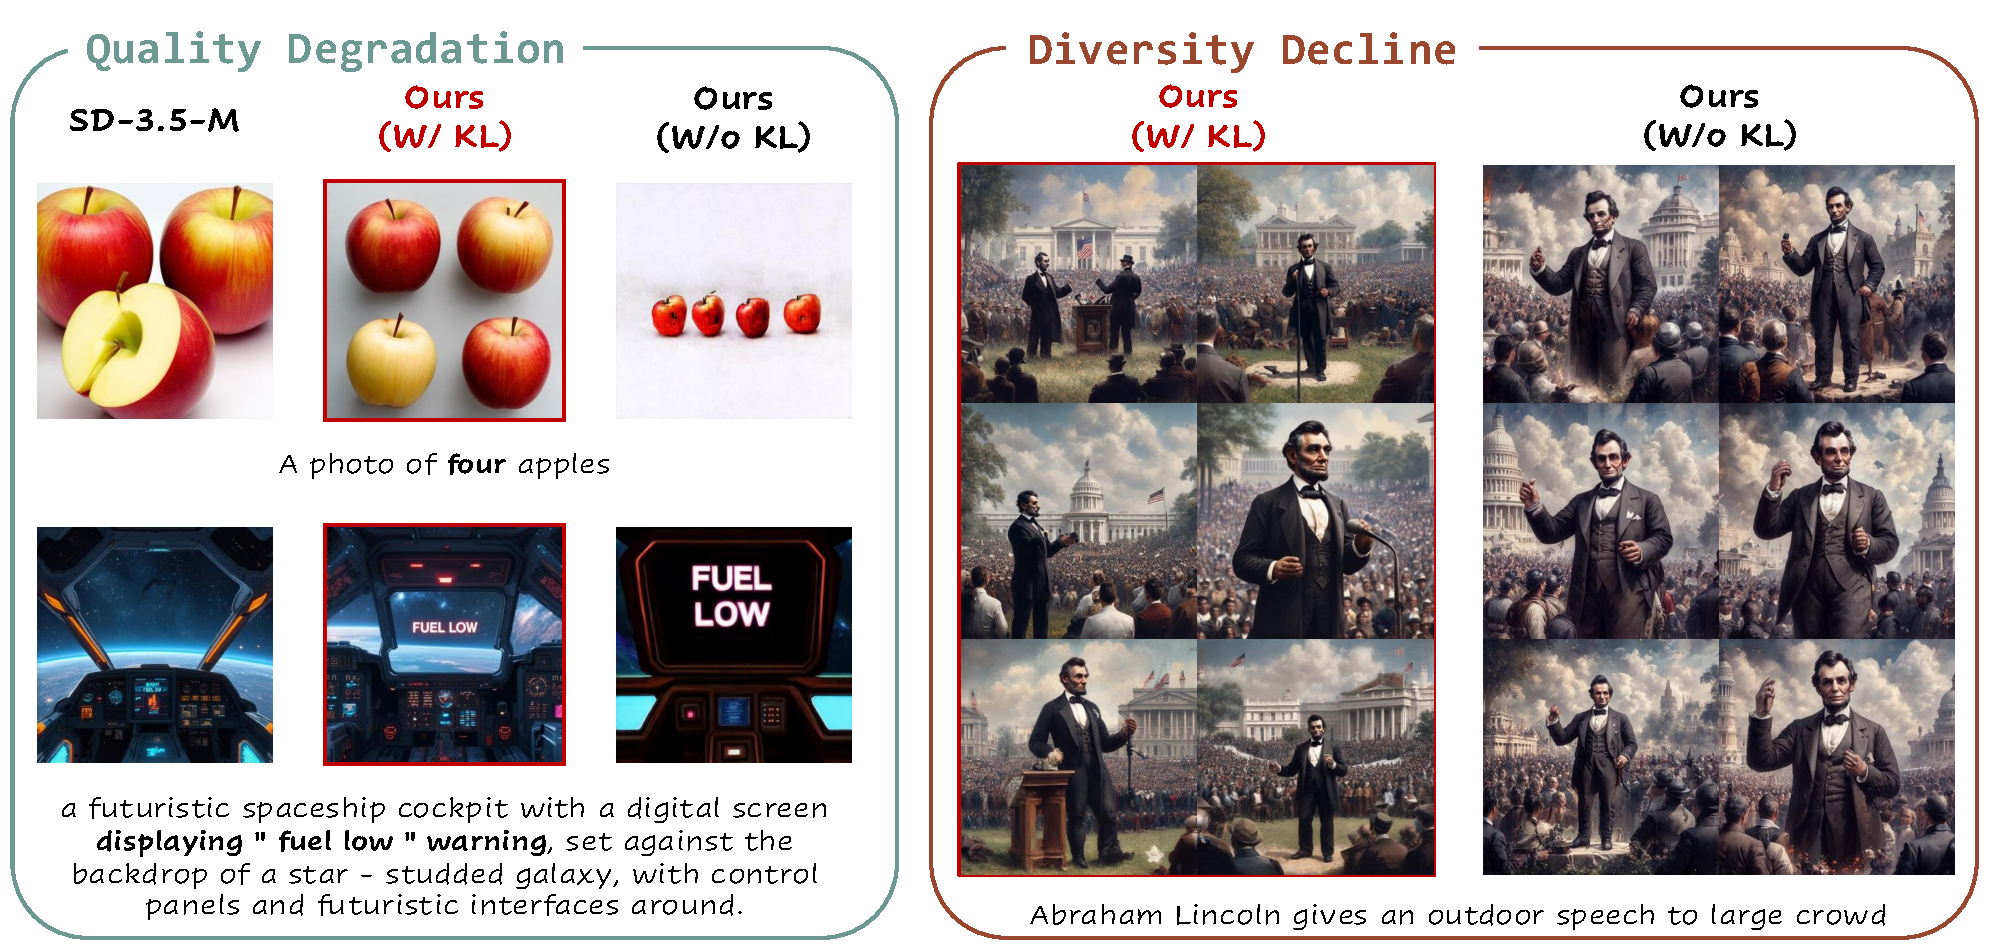
\includegraphics[width=\textwidth]{src/experiments/ablation_kl.pdf}
\caption{\textbf{Effect of KL Regularization.} The KL penalty effectively suppresses reward hacking, preventing
\textbf{\textcolor{pltpos}{Quality Degradation}} (for GenEval and OCR) and  
\textbf{\textcolor{pltattr}{Diversity Decline}} (for PickScore).
}
\vspace{-3mm}
\label{fig:quality_divesity_example}
\end{figure}

\paragraph{Effect of Denoising Reduction.}
Figure~\ref{fig:exp_ablation} (a) highlights Denoising Reduction's significant impact on accelerating training. To explore how different timesteps affect optimization, these experiments are conducted without the KL constraint. Reducing data collection timesteps from $40$ to $10$ achieves over a $4\times$ speedup across all three tasks, without impacting final reward. Further reducing to $5$ does not consistently improve speed and sometimes slows training, so we choose $10$ timesteps for later experiments. For the other two tasks, learning curves of reward versus training time are presented in Figure~\ref{app:fig:exp2_ablation_step} in the Appendix~\ref{app:subsec:noising_reduction}.



\paragraph{Effect of Noise Level.}\label{sec:exp:noise_scheduler}
% 提高SDE中的$\sigma_t$可以给生成的图片带来更多的多样性，从而提升exploration，这对rl训练至关重要。As in Eq.~\ref{eq:update_rule}, we control the exploration by the Noise level 系数$a$.
% We conduct ablations to study how the noise level $a$ influences performance. Figure~\ref{} presents results for different values of $a$. Small noise levels (e.g., $a = 0.1$) limit exploration and lead to slow reward improvement. Increasing $a$ (up to 0.7) enhances exploration and accelerates reward gains. However, beyond a certain point, further increasing the noise (e.g., $a = 0.7\rightarrow1.0$) brings no additional benefit as the exploration space is already sufficient for learning. We also observe that overly large noise levels severely degrade image quality, causing the reward to remain at zero and preventing effective training. We recommend using the highest noise level that does not significantly harm image quality.
Higher $\sigma_t$ in the SDE boosts image diversity and exploration, vital for RL training. We control this exploration with a noise level $a$ (Eq.~\ref{eq:update_rule}).
Figure~\ref{fig:exp_ablation} (b) shows the impact of $a$ on performance. A small $a$ (e.g., 0.1) limits exploration and slows reward improvement. Increasing $a$ (up to 0.7) boosts exploration and speeds up reward gains. Beyond this point (e.g., from 0.7 to 1.0), further increases provide no additional benefit, as exploration is already sufficient. We also observe that injecting too much noise by further increasing $a$ degrades image quality, resulting in zero reward and failed training. 

\begin{figure}[htbp]
  \centering
  \begin{minipage}[t]{0.48\textwidth}
    \centering
    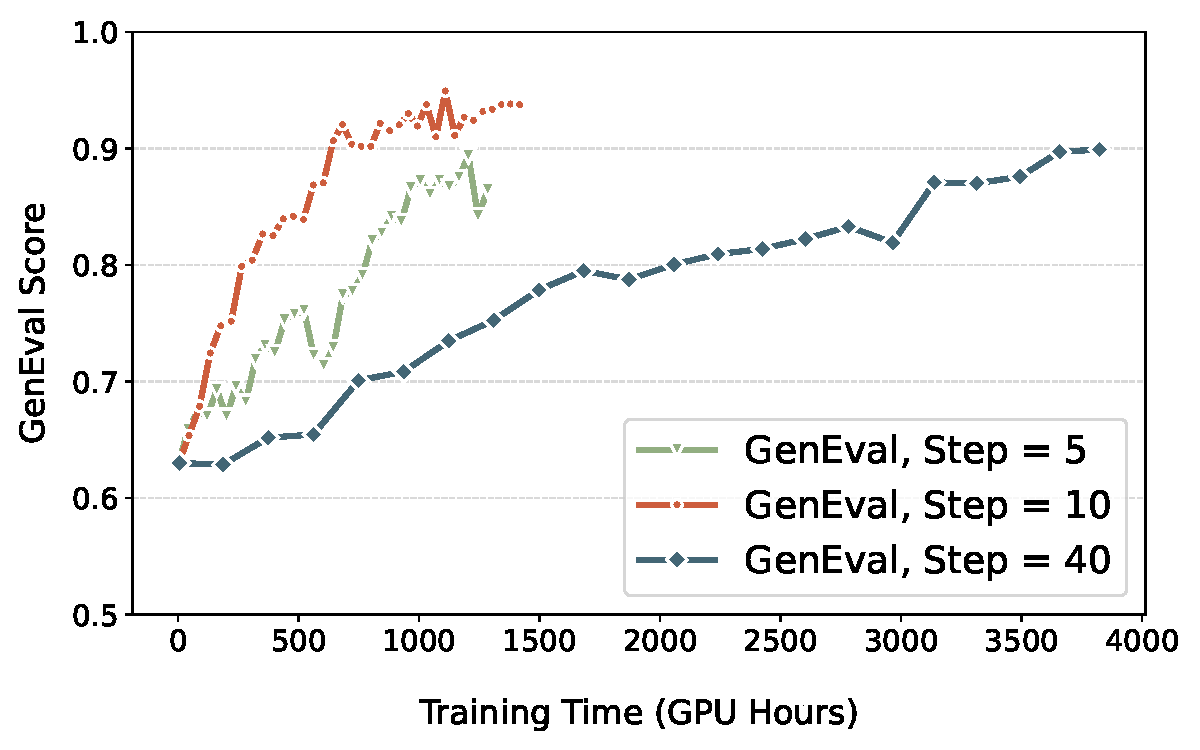
\includegraphics[width=\linewidth]{src/experiments/ablation_step/exp2_geneval_ablation_step.pdf}
    \vspace{-1.5em}
    \caption*{\footnotesize (a). Effect of Denoising Reduction on GenEval}
  \end{minipage}
  \hfill
  \begin{minipage}[t]{0.48\textwidth}
    \centering
    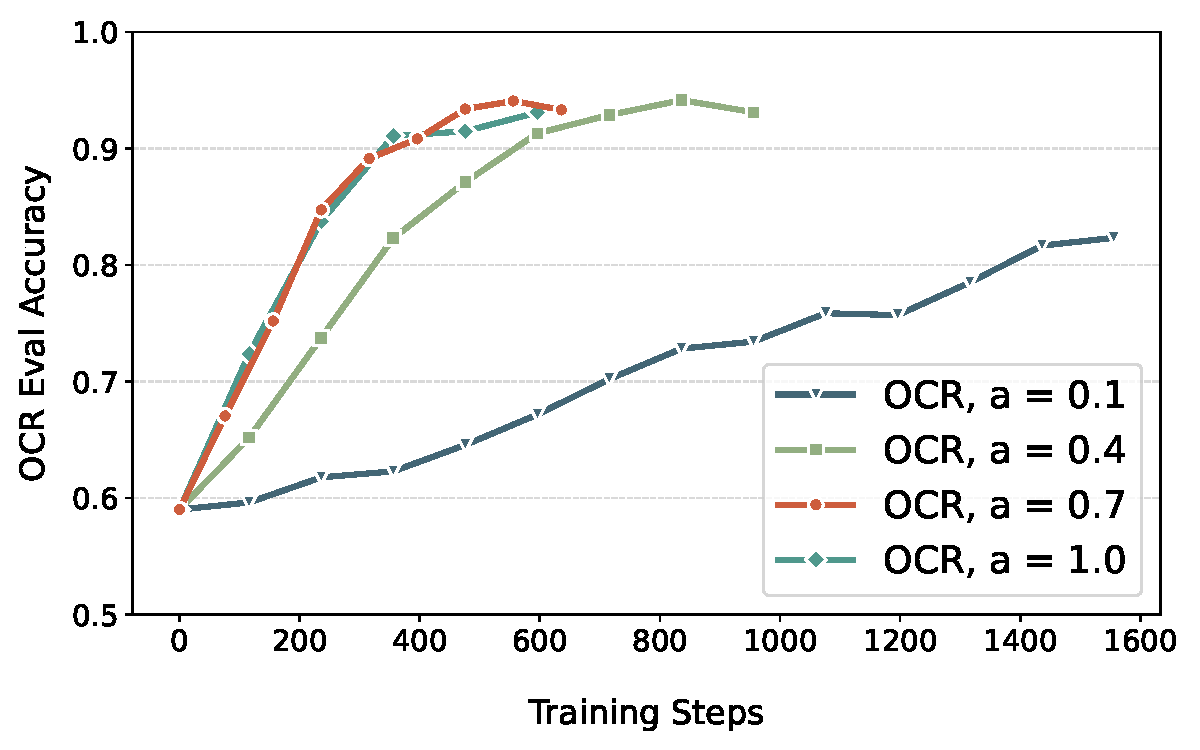
\includegraphics[width=\linewidth]{src/experiments/ablation_noise/exp1_ocr_ablation_noise.pdf}
    \vspace{-1.5em}
    \caption*{\footnotesize (b). Effect of Noise Level Ablation on the OCR}
  \end{minipage}
  % \begin{minipage}[t]{0.48\textwidth}
  %   \centering
  %   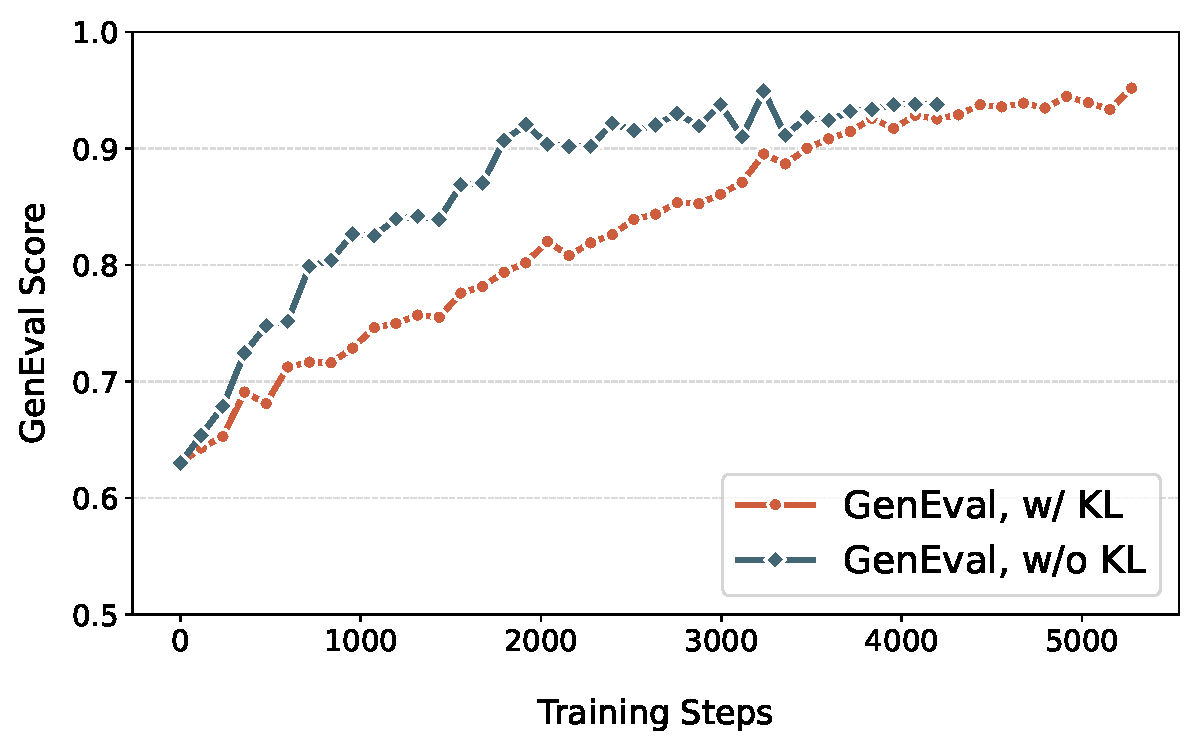
\includegraphics[width=\linewidth]{src/experiments/ablation_kl/exp3_geneval_ablation_kl.pdf}
  %   \vspace{-1.5em}
  %   \caption*{\footnotesize (b). Effect of KL‑Regularization on GenEval}
  % \end{minipage}
  % \vspace{1.5em}

  \caption{
  Ablation studies on our critical design choices. 
  \textbf{(a) Denoising Reduction}: Fewer denoising steps accelerate convergence and yield similar performance.
  % \textbf{(b) KL-Regularization}: KL penalty slows early training yet effectively suppresses reward hacking.
  \textbf{(b) Noise Level:} Moderate noise level ($a = 0.7$) maximises OCR accuracy, while too little noise hampers exploration.
  }
  \vspace{-2mm}
  \label{fig:exp_ablation}
\end{figure}

\paragraph{Effect of Group Size.}\label{sec:exp:group_number}
Figure~\ref{fig:abltion_groupsize} shows the effect of group size $G$ using PickScore as the reward function. When the group size was reduced to $G=12$ and $G=6$, training became unstable and eventually collapsed, whereas $G=24$ remained stable throughout the process. We observe that smaller group sizes produce inaccurate advantage estimates, increasing variance and leading to training collapse, a phenomenon also reported in~\cite{liu2025prorl,chen2025acereason}.

\paragraph{Generalization Analysis.}
Flow-GRPO demonstrates strong generalization on unseen scenarios from GenEval (Table~\ref{tab:geneval_unseen}). Specifically, it captures object number, color, and spatial relations, generalizing well to unseen object classes. It also effectively controls object count, generalizing from training on $2-4$ objects to generate $5-6$ or $12$ objects. Furthermore, Table~\ref{tab:t2i_comp_bench} shows Flow-GRPO achieves significant gains on T2I-CompBench++~\cite{T2i-compbench, huang2025t2i}. This comprehensive benchmark for open-world compositional T2I generation features object classes and relationships substantially different from our model's GenEval-style training data.

% \begin{table}[]
% \centering
%     \caption{\textbf{Flow-GRPO demonstrates strong generalization.} Unseen Obj.: Trained on 60 object classes, evaluated on 20 unseen classes. Unseen Attr. Binding: The model from Figure~\ref{fig:teaser} is evaluated on 10 unseen colors. Unseen Counting: The same model from Figure~\ref{fig:teaser}, initially trained to render 2, 3, or 4 objects, was evaluated on rendering 5 or 6.}
% \begin{tabular}{lccc}
% \toprule
% \multicolumn{1}{l}{} & Unseen Obj. & Unseen Attr. Binding & Unseen Counting \\ \midrule
% SD3-M                & 0.60            & 0.34              & 0.14            \\
% SD3-M+Flow-GRPO      & 0.83           & 0.57              & 0.45            \\ \bottomrule
% \end{tabular}
% \label{tab:geneval_unseen}
% \end{table}

\begin{table}[h]
\centering
\small
    \caption{{\bf T2I-CompBench++ Result.} This evaluation uses the same model presented in Table~\ref{tab:geneval}, which was trained on the GenEval-generated dataset.
The best score is in \colorbox{pearDark!20}{blue}.}
\resizebox{\linewidth}{!}{
\begin{tabular}{lccccccc}
\toprule
\textbf{Model} & \textbf{Color} & \textbf{Shape} & \textbf{Texture} & \textbf{2D-Spatial} & \textbf{3D-Spatial} & \textbf{Numeracy} & \textbf{Non-Spatial} \\ \midrule
Janus-Pro-7B~\cite{chen2025janus}  & 0.5145 & 0.3323 &0.4069 & 0.1566 & 0.2753 & 0.4406 & 0.3137 \\
EMU3~\cite{wang2024emu3} & 0.7913 & 0.5846 & \colorbox{pearDark!20}{0.7422} & — & — & — & — \\
FLUX.1 Dev~\cite{flux2024}         & 0.7407 & 0.5718 & 0.6922 & 0.2863 & 0.3866 & 0.6185 & 0.3127 \\
SD3.5-M~\cite{sd3}           & 0.7994 & 0.5669 & 0.7338 & 0.2850  & 0.3739 & 0.5927 & 0.3146 \\
\textbf{SD3.5-M+Flow-GRPO} & \colorbox{pearDark!20}{0.8379} & \colorbox{pearDark!20}{0.6130} & 0.7236 & \colorbox{pearDark!20}{0.5447} & \colorbox{pearDark!20}{0.4471} & \colorbox{pearDark!20}{0.6752} & \colorbox{pearDark!20}{0.3195} \\ \bottomrule
\end{tabular}
}
\vspace{-2mm}
\label{tab:t2i_comp_bench}
\end{table}

\begin{table}[h]
\centering
    \caption{\textbf{Flow-GRPO demonstrates strong generalization.} Unseen Objects: Trained on 60 object classes, evaluated on 20 unseen classes. Unseen Counting: Trained to render 2, 3, or 4 objects, and evaluated in two settings: rendering 5 or 6 objects, and rendering 12 objects.}
\resizebox{\linewidth}{!}{
\begin{tabular}{lccccccccc}
\toprule
\multirow{2}{*}{\textbf{Method}} & \multicolumn{7}{c}{\textbf{Unseen Objects}}                                              & \multicolumn{2}{c}{\textbf{Unseen Counting}} \\ \cmidrule(lr){2-8} \cmidrule(l){9-10} 
                        & \textbf{Overall} & \textbf{Single Obj.} & \textbf{Two Obj.} & \textbf{Counting} & \textbf{Colors} & \textbf{Position} & \textbf{Attr. Binding} & \textbf{5$-$6 Objects} &\textbf{12 Objects}        \\ \midrule
SD3.5-M                   & 0.64    & 0.96        & 0.73     & 0.53     & 0.87   & 0.26     & 0.47          & 0.13    & 0.02              \\
\textbf{SD3.5-M+Flow-GRPO}         & \colorbox{pearDark!20}{0.90}        & \colorbox{pearDark!20}{1.00}        & \colorbox{pearDark!20}{0.94}         & \colorbox{pearDark!20}{0.86}         & \colorbox{pearDark!20}{0.97}       & \colorbox{pearDark!20}{0.84}         & \colorbox{pearDark!20}{0.77}              & \colorbox{pearDark!20}{0.48}      & \colorbox{pearDark!20}{0.12}           \\ \bottomrule
\end{tabular}
}
\vspace{-2mm}
\label{tab:geneval_unseen}
\end{table}

% This structure emphasizes methodological generality while highlighting task-specific insights, ensuring reproducibility through hyperparameter transparency and ablation rigor.
% \section{Discussion}\label{sec:dis}
% We have presented weak-to-strong search, an alignment method that keeps the large language model frozen while steering its decoding through a test-time greedy search over small language models.
% This method builds on the insight that the log-probability difference between small tuned and untuned language models can serve both as a dense reward function and a value function, and then introduces a novel beam search algorithm designed for balancing reward maximization and KL minimization.
% This method offers a compute-efficient model up-scaling strategy that eliminates the complexity of directly fine-tuning the large models, and exemplifies weak-to-strong generalization~\cite{burns2023weak} that makes strong models stronger with only weak test-time guidance.
% Empirically, this approach is effective in controlled-sentiment generation, summarization, and instruction following.

\section{Conclusion}
We have presented Flow-GRPO, the first method to integrate online policy gradient RL into flow matching models. By converting deterministic ODEs to SDEs and reducing denoising steps during training, Flow-GRPO enables efficient RL-based optimization without noticeably compromising image quality or diversity.
Our method significantly improves performance on compositional generation, text rendering, and human preference alignment, with minimal reward hacking. Flow-GRPO offers a simple and general framework for applying online RL to flow-based generative models.

\label{sec:limitation}
\paragraph{Limitations \& Future Work.} 
Although this work focuses on T2I tasks, Flow-GRPO has potential for video generation~\cite{wanx, hunyuanvideo}, raising several future directions: (1) Reward Design: Simple heuristics, such as using object detectors or trackers as rule-based rewards, can encourage physical realism and temporal consistency, but more advanced reward models are needed.
(2) Balancing Multiple Rewards: Video generation requires optimizing multiple objectives, including realism, smoothness, and coherence. Balancing these competing goals remains challenging and demands careful tuning.
(3) Scalability: Video generation is far more resource-intensive than T2I, so applying Flow-GRPO at scale requires more efficient data collection and training pipelines. Additionally, better methods for preventing reward hacking are worth exploring. While KL regularization helps significantly, it requires longer training and occasional reward hacking occurs for certain prompts.

\section*{Acknowledgements}
This work was partially supported by the JC STEM Lab of AI for Science and Engineering, funded by The Hong Kong Jockey Club Charities Trust, the Research Grants Council of Hong Kong (Project No. CUHK14213224).
We gratefully acknowledge Mingwu Zheng for his insightful discussions on the proof and Zhanhui Zhou for his valuable comments that improved the clarity of this paper.

% Denoising Reduction is a promising
% Our experiments in Section~\ref{sec:exp:distill} also suggest Flow-GRPO can be used for distillation. Future work may explore using it to train compact T2I models with fewer sampling steps.
% \section*{Acknowledgements}
% This work was supported in part by the National Key R\&D Program of China (NO.2022ZD0160201). We would like to thank anonymous reviewers for their valuable feedback and helpful discussions.

% \section*{Author Contributions}
% \textbf{Zhanhui Zhou}  led the project, proposed the research idea, wrote the codebase, designed the experiments, conducted most of the initial experiments, and wrote the paper. \textbf{Zhixuan Liu} assisted with running many of the ablation studies throughout the experiments presented in the paper. All other authors provided feedback throughout the project.


% \clearpage
\bibliography{
references/flowpo,
references/alignment, 
references/search,
references/proxy_tuning,
references/models,
references/benchmarks,
references/others
}

\clearpage
\appendix
\appendixtitle

% \setcounter{page}{1}
% \setcounter{section}{0}
% \setcounter{figure}{0}
% \setcounter{table}{0}

\startcontents[app]
\printcontents[app]{l}{1}{%
  % \section*{\centering Appendix}%
}{}

% \etocsettocstyle{\noindent}{}
% \etocsetnexttocdepth{2}
% \localtableofcontents


% \renewcommand{\contentsname}{}
% \tableofcontents

% \minitoc 

\vspace{1em}

\noindent Our Appendix consists of 4 sections. Readers can click on each section number to navigate to the corresponding section:
\vspace{-0.6em}
\begin{itemize}[leftmargin=2.0em]
    \item Section~\ref{app:sec:math} provides detailed derivations of stochastic sampling in flow matching models.
    \item Section~\ref{app:sec:exp-setup-details} presents details about our experimental setup.
    \item Section~\ref{app:sec:extened-exp-results} offers some additional experimental results, including 1) the comparison with other alignment methods, 2) ablation of denoising reduction on OCR accuracy and pickscore, 3) ablation of initial noise, 4) additional results on FLUX.1-Dev, 5) the learning curves of Flow-GRPO on three tasks, 6) additional qualitative results, and 7) evolution of evaluation images during training.
    \item Section~\ref{app:sec:denoising_reduction_viz} provides a visualization of training samples under the denoising reduction strategy.
    
\end{itemize}
\vspace{-0.4em}

In addition to this Appendix, we also provide more visualization results, see \href{https://gongyeliu.github.io/Flow-GRPO/}{this website}. We encourage the readers to consult this HTML page for a more intuitive assessment of the improvements brought by Flow-GRPO.

% \iftoggle{isSubmission}{
%  In addition to this Appendix, we also provide \textbf{a local HTML for image comparisons}. We encourage the reviewers to consult this HTML file for a more intuitive assessment of the improvements brought by Flow-GRPO.
% }
%  For more visualization results, see \href{https://gongyeliu.github.io/Flow-GRPO/}{this website}.
\clearpage
\input{sections/appendix/math}
% \iftoggle{isSubmission}{}
% {\section{Changelog}
% \textbf{v1}: We corrected an evaluation inconsistency: using $\text{top-k} = 50$ for regular decoding (i.e., Base) and EFT, but $\text{top-k} = \infty$ for BoN and weak-to-strong search, which had \textit{slightly} underestimated results for weak-to-strong and BoN. This version standardizes $\text{top-k} = 50$ and updates results from the previous version (the version under review).

% \textbf{v2}: We fixed an error in our plots where we had incorrectly shown variances instead of standard deviations.
% }
% \clearpage
\section{Further Details on the Experimental Setup}\label{app:sec:exp-setup-details}

\subsection{Quality Metrics}\label{app:subsubsec:quality_metric}
The details of quality metrics are as follows:
\begin{itemize} [leftmargin=15pt]
  \item Aesthetic score~\cite{schuhmann2022laion}: a CLIP‑based linear regressor that predicts an image’s aesthetic score.
  \item DeQA score~\cite{deqa}: a multimodal large language model based image‑quality assessment (IQA) model that quantifies how distortions, texture damage, and other low‑level artefacts affect perceived quality.
  \item ImageReward~\cite{xu2024imagereward}: a general purpose T2I human preference reward model that captures text–image alignment, visual fidelity, and harmlessness.
  \item UnifiedReward~\cite{wang2025unified}: a recently proposed unified reward model for multimodal understanding and generation that currently achieves state‑of‑the‑art performance on the human preference assessment leaderboard.
\end{itemize}

\subsection{Model Specification}\label{app:subsubsec:synthetic-model}
The following table lists the base model and the reward models and their corresponding links.

\begin{table}[h]
\centering
\resizebox{\linewidth}{!}{
\begin{tabular}{ll}
\toprule
\textbf{Models} & \textbf{Links} \\
\midrule
\texttt{SD3.5-M}~\citep{sd3} & \url{https://huggingface.co/stabilityai/stable-diffusion-3.5-medium} \\
\texttt{Aesthetic Score}~\citep{schuhmann2022laion} & \url{https://github.com/LAION-AI/aesthetic-predictor} \\
\texttt{PickScore}~\citep{kirstain2023pick} & \url{https://huggingface.co/yuvalkirstain/PickScore_v1} \\
\texttt{DeQA score}~\citep{deqa} & \url{https://huggingface.co/zhiyuanyou/DeQA-Score-Mix3} \\
\texttt{ImageReward}~\citep{xu2024imagereward} & \url{https://huggingface.co/THUDM/ImageReward} \\
\texttt{UnifiedReward}~\citep{wang2025unified} & \url{https://huggingface.co/CodeGoat24/UnifiedReward-7b-v1.5} \\
\bottomrule
\end{tabular}
}
\end{table}




\subsection{Hyperparameters Specification}\label{app:subsubsec:synthetic-hyperp}
Except for $\beta$, GRPO hyperparameters are fixed across tasks. We use a sampling timestep $T=10$ and an evaluation timestep $T=40$. Other settings include a group size $G=24$, an noise level $a=0.7$ and an image resolution of 512. The KL ratio $\beta$ is set to 0.04 for GenEval and Text Rendering, and 0.01 for Pickscore. We use Lora with $\alpha=64$ and $r=32$.

\subsection{Compute Resources Specification}\label{app:subsubsec:synthetic-compute}
We train our model using 24 NVIDIA A800 GPUs. The learning curves in Appendix~\ref{app:subsec:training_curve_kl} provide details on the specific GPU hours.

% \subsubsection{Gold Reward Model Details}\label{app:subsubsec:synthetic-grm}
% % \begin{longtable}{lll} 
% % \toprule
% % \textbf{Tasks} & \textbf{Models} & \textbf{Links} \\
% % \midrule
% % \texttt{IMDB} & \texttt{lvwerra/distilbert-imdb} (268M) & \url{https://huggingface.co/lvwerra/distilbert-imdb} \\
% % \texttt{Summarize} & \texttt{chadlzx/summarize-goldenrm-llama-2-7b} & \url{https://huggingface.co/chadlzx/summarize-goldenrm-llama-2-7b} \\
% % \bottomrule
% % \end{longtable}

% % In our research, the gold reward model was utilized for two specific tasks: controlled-sentiment generation and summarization.

% % For controlled-sentiment generation, the model deployed was \texttt{lvwerra/distilbert-imdb}, a fine-tuned version of \texttt{distilbert-base-uncased} on the \texttt{IMDB} dataset, featuring 66 million parameters.

% % In the summarization task, training was executed within the \texttt{SafeRLHF} framework using the \texttt{llama-2-7b} model, on the \texttt{CarperAI/openai\_summarize\_comparisons} dataset. Training configurations included $bs=32$, $lr=1 \times 10^{-5}$ for new parameters and $lr=5 \times 10^{-6}$ for pre-trained parameters, over a single epoch with a cosine learning rate schedule.

% % \todo{
% We follow the synthetic setup in which we use the gold reward models to play the roles of humans and provide binary preference labels~\cite{gao2023scaling, lightman2023let, rafailov2024direct}. 
% % \iftoggle{isSubmission}{}
% % {We list the links to the two gold reward models in the following table:
% % \vspace{-5mm}
% % \begin{center}
% % \resizebox{1\linewidth}{!}{
% % \begin{tabular}{ll}
% % \toprule
% % \textbf{Models} & \textbf{Links} \\
% % \midrule
% % \texttt{distilbert-imdb} (268M) & \url{https://huggingface.co/lvwerra/distilbert-imdb} \\
% % \texttt{summarize-goldrm-llama-2-7b} & \url{https://huggingface.co/chadlzx/summarize-goldrm-llama-2-7b} \\
% % \bottomrule
% % \end{tabular}
% % }
% % \end{center}
% % }

% For controlled-sentiment generation, we reuse the publicly available \href{https://huggingface.co/lvwerra/distilbert-imdb}{\texttt{distilbert-imdb}} to define the gold reward model $r_{\text{gold}}$. \href{https://huggingface.co/lvwerra/distilbert-imdb}{\texttt{Distilbert-imdb}} is a fine-tuned classifier $p$ on the \href{https://huggingface.co/datasets/stanfordnlp/imdb}{\texttt{imdb}} dataset~\cite{maas-etal-2011-learning} to classify movie review sentiments.
% We define the gold reward $r_{\text{gold}}$ as $\log p(\text{positive} \, | \, x, y) - \log p (\text{negative} \, | \, x, y)$ to encourage positive review. 
% % We then collect synthetic preferences from the gold reward model $\mathcal{D} = \{(\rvx, \rvy_w, \rvy_l)_i \}_{i=1}^N$.
% % The prompt set consists of prefixes of movie reviews (i.e., truncated movie reviews) and for each prefix $\rvx$, we sample pairwise completions $\rvy_1, \rvy_2$ from \href{https://huggingface.co/lvwerra/gpt2-imdb}{\texttt{gpt2-imdb}}, a publically available language model fine-tuned on \texttt{imdb} dataset. These pairwise responses are then ranked by the $r_{\text{gold}}$ with $p(\rvy_1 \succ \rvy_2 \mid \rvx) = \sigma (r_{\text{gold}}(\rvx, \rvy_1) - r_{\text{gold}}(\rvx, \rvy_2))$.
% Synthetic preferences are collected using the truncated movie reviews as prompts $\rvx$, and pairwise completions from \href{https://huggingface.co/lvwerra/gpt2-imdb}{\texttt{gpt2-imdb}}, ranked with $p(\rvy_1 \succ \rvy_2 \mid \rvx) = \sigma (r_{\text{gold}}(\rvx, \rvy_1) - r_{\text{gold}}(\rvx, \rvy_2))$, as preferences.


% For summarization, we fit a reward model on the \href{https://huggingface.co/datasets/openai/summarize_from_feedback}{\texttt{summarize\_from\_feedback}} dataset~\cite{stiennon2020learning} as the gold reward model $r_{\text{gold}}$. 
% Specifically, this reward model is fine-tuned from \texttt{Llama-2-7b} with a linear projection head and binary cross entropy loss, using a batch size of $32$, a learning rate of \texttt{1e-5} for the projection head, and \texttt{5e-6} for other parameters, over one epoch with a cosine learning rate schedule. 
% Synthetic preferences are generated by relabeling pairwise responses in the original dataset with $p(\rvy_1 \succ \rvy_2 \mid \rvx) = \sigma (r_{\text{gold}}(\rvx, \rvy_1) - r_{\text{gold}}(\rvx, \rvy_2))$.
% % To collect synthetic preferences from the gold reward model, we relabel the pairwise responses in the original dataset by the gold reward model with $p(\rvy_1 \succ \rvy_2 \mid \rvx) = \sigma (r_{\text{gold}}(\rvx, \rvy_1) - r_{\text{gold}}(\rvx, \rvy_2))$.

% Both gold reward models show high validation accuracies, $0.928$ and $0.736$, demonstrating strong correlation with human judgments.

% \subsubsection{Direct Tuning Details}\label{app:subsubsec:synthetic-tuning-details}
% % We detail the finetuning strategies for four language models—\texttt{gpt2-large}, \texttt{gpt2-xl}, \texttt{llama-2-7B}, and \texttt{llama-3-8B}—targeting controlled-sentiment generation and summarization. The procedure includes two phases: Supervised Fine-Tuning (\texttt{SFT}) and Direct Preference Optimization (\texttt{DPO}).

% % During the \texttt{SFT} phase, models underwent finetuning on \texttt{IMDB} for sentiment control and \texttt{CarperAI/openai\_summarize\_tldr} for summarization, with parameters set to $lr=2e-5$, $bs=64$, and $epochs=1$, employing a cosine scheduler.

% % In the \texttt{DPO} phase, using the gold reward model, the models were retrained on relabeled data from the same datasets. Settings were adjusted to $lr=1e-6$, $bs=256$, $\beta=0.1$, and $epochs=1$, again utilizing a cosine scheduler for dynamic learning rate adjustments.
% Direct tuning on the synthetic preferences $\mathcal{D} = \{(\rvx, \rvy_w, \rvy_l)_i \}_{i=1}^N$ involves two stages: Supervised Fine-Tuning (\texttt{SFT}) and Direct Preference Optimization (\texttt{DPO})~\cite{rafailov2024direct}. During \texttt{SFT}, models are trained on both selected and rejected responses using a batch size of $64$, a learning rate of \texttt{2e-5}, and a cosine learning rate schedule over one epoch. During \texttt{DPO}, we use a $\beta=0.1$, batch size of $256$, a learning rate of \texttt{1e-6}, and a cosine learning rate schedule over one epoch.


% \subsubsection{Prompt Template for Sampling from Base Models}\label{app:subsubsec:synthetic-prompt-template}
% When sampling from large pre-trained models, it is crucial to provide clear task-specific instructions. 
% For sentiment-controlled generation, we use a zero-shot prompt:

% % \begin{Verbatim}[frame=single]
% % BEGINNING OF CONVERSATION: USER: {system prompt}{query} ASSISTANT:
% % \end{Verbatim}
% \begin{center}
% \verb|Here is a movie review from imdb: {prompt}|
% \end{center}

% For summarization, we use a two-shot prompt (the exemplars are selected arbitrarily):

% \begin{Verbatim}
%               {examplar[1].prompt}TL;DR: {examplar[1].response}
%               {examplar[2].prompt}TL;DR: {examplar[2].response}
%               {prompt}TL;DR: 
% \end{Verbatim}


% \subsection{Instruction Following}\label{app:subsec:exp-setup-details-instruction-following}

% \subsubsection{Model Specification}\label{app:subsubsec:instruction-following-model}
% The following table lists the models and their corresponding links.

% % {
% % \footnotesize
% % \begin{longtable}{ll}
% % \toprule
% % \textbf{Models} & \textbf{Links} \\
% % \midrule
% % \texttt{zephyr-7b-beta}~\cite{tunstall2023zephyr} & \url{https://huggingface.co/HuggingFaceH4/zephyr-7b-beta} \\
% % \texttt{mistral-7b-sft-beta}~\cite{tunstall2023zephyr} & \url{https://huggingface.co/HuggingFaceH4/mistral-7b-sft-beta} \\
% % \texttt{tulu-2-dpo-7b}~\cite{ivison2023camels} & \url{https://huggingface.co/allenai/tulu-2-dpo-7b} \\
% % \texttt{tulu-2-7b}~\cite{ivison2023camels} & \url{https://huggingface.co/allenai/tulu-2-7b} \\
% % \texttt{Llama-2-7b-chat}~\cite{touvron2023llama2} & \url{https://huggingface.co/meta-llama/Llama-2-7b-chat-hf} \\
% % \texttt{Llama-2-70b-chat}~\cite{touvron2023llama2} & \url{https://huggingface.co/meta-llama/Llama-2-70b-chat-hf} \\
% % \texttt{Llama-3-8B-Instruct}~\cite{llama3modelcard} & \url{https://huggingface.co/meta-llama/Meta-Llama-3-8B-Instruct} \\
% % \texttt{Llama-3-70B-Instruct}~\cite{llama3modelcard} & \url{https://huggingface.co/meta-llama/Meta-Llama-3-70B-Instruct} \\
% % \texttt{gpt-3.5-turbo-instruct}~\cite{ouyang2022training} & \url{https://platform.openai.com/docs/models/gpt-3-5-turbo} \\
% % \bottomrule
% % \end{longtable}
% % }

% \begin{center}
% \resizebox{1\linewidth}{!}{
% \begin{tabular}{ll}
% \toprule
% \textbf{Models} & \textbf{Links} \\
% \midrule
% \texttt{zephyr-7b-beta}~\cite{tunstall2023zephyr} & \url{https://huggingface.co/HuggingFaceH4/zephyr-7b-beta} \\
% \texttt{mistral-7b-sft-beta}~\cite{tunstall2023zephyr} & \url{https://huggingface.co/HuggingFaceH4/mistral-7b-sft-beta} \\
% \texttt{tulu-2-dpo-7b}~\cite{ivison2023camels} & \url{https://huggingface.co/allenai/tulu-2-dpo-7b} \\
% \texttt{tulu-2-7b}~\cite{ivison2023camels} & \url{https://huggingface.co/allenai/tulu-2-7b} \\
% \texttt{Llama-2-7b-chat}~\cite{touvron2023llama2} & \url{https://huggingface.co/meta-llama/Llama-2-7b-chat-hf} \\
% \texttt{Llama-2-70b-chat}~\cite{touvron2023llama2} & \url{https://huggingface.co/meta-llama/Llama-2-70b-chat-hf} \\
% \texttt{Llama-3-8B-Instruct}~\cite{llama3modelcard} & \url{https://huggingface.co/meta-llama/Meta-Llama-3-8B-Instruct} \\
% \texttt{Llama-3-70B-Instruct}~\cite{llama3modelcard} & \url{https://huggingface.co/meta-llama/Meta-Llama-3-70B-Instruct} \\
% \texttt{gpt-3.5-turbo-instruct}~\cite{ouyang2022training} & \url{https://platform.openai.com/docs/models/gpt-3-5-turbo} \\
% \bottomrule
% \end{tabular}
% }
% \end{center}

% \subsubsection{Hyperparameters Specification}\label{app:subsubsec:instruction-following-hyperparam}
% When sampling from \texttt{Llama-3-8B-Instruct} and \texttt{Llama-3-70B-Instruct}, we use the $T=0.6$, $\text{top-k} = 1.0$ and $\text{top-p} = 0.9$ as per the official Llama-3 generation \href{https://huggingface.co/meta-llama/Meta-Llama-3-8B-Instruct/blob/main/generation_config.json}{configuration}. For other models, we default to temperature $T=0.7$, $\text{top-k} = 50$ and $\text{top-p} = 1.0$. Specific hyperparameters for each method are detailed in Tables~\ref{tab:zephyr-guidance} and~\ref{tab:tulu-guidance}. 
% % Generally, for small open-source models (7B \& 8B), we use $W,K,L=4,4,30$ ($W$: beam width, $K$: successors per state, $L$: chunk length) for weak-to-strong search (CBS), and $N=16$ for BoN; for large open-source models (70B), we use $W,K,L=2,2,30$ for weak-to-strong search (CBS), and $N=4$ for BoN; for black-box models, we use $W,K,L=2,2,100$ for weak-to-strong search (CBS), and $N=4$ for BoN.

% \subsubsection{Compute Resources Specification}\label{app:subsubsec:instruction-following-compute}
% Models are evaluated on 805 test prompts. Model inference takes place on one single NVIDIA A100 GPU for 7B\&8B and black-box models, and on four NVIDIA A100 GPUs for 70B models.
% % \todo{...}
% % We inference on 
\section{Extended Experimental Results}\label{app:sec:extened-exp-results}

\subsection{Flow-GRPO vs. Other Alignment Methods}\label{app:subsec:baselines}
We compare Flow-GRPO with several alignment methods: supervised fine-tuning (SFT), reward-weighted regression (Flow-RWR~\cite{videoalign, awr}), Flow-DPO~\cite{videoalign}, and their online variants. Flow-GRPO consistently outperforms all baselines by a significant margin.
At each step, we generate a group of images using the same group size as in Flow-GRPO. The only difference lies in the update rule:
\begin{itemize}
\setlength{\itemindent}{-2em}
\item \textbf{SFT}: Select the highest-reward image in each group and fine-tune on it.
\item \textbf{Flow-RWR}~\cite{videoalign, awr}: Apply a softmax over rewards in each group and perform reward-weighted likelihood maximization.
\item \textbf{Flow-DPO}~\cite{videoalign,wallace2024diffusion}: Use the highest-reward image in each group as the chosen sample and the lowest as the rejected, then apply the DPO loss.
\end{itemize}

Offline variants use a fixed pretrained model for data collection, while online variants update their data collection model every 40 steps. As shown in Figure~\ref{app:fig:compare_curva}, Flow-GRPO outperforms all other methods. The figure also indicates that DPO and SFT improve over time. In contrast, RWR does not, which aligns with experimental findings on RWR in~\cite{ddpo}. Additionally, Online DPO surpasses offline DPO, aligning with~\cite{skyreels_v2}'s finding that online DPO performs better. For the second-best online DPO, a hyperparameter search on its key parameter $\beta$ revealed that smaller values are not always optimal; excessively small $\beta$ values can cause training collapse.


\begin{figure}[htbp]
  \centering
  \begin{minipage}[t]{\textwidth}
    \centering
    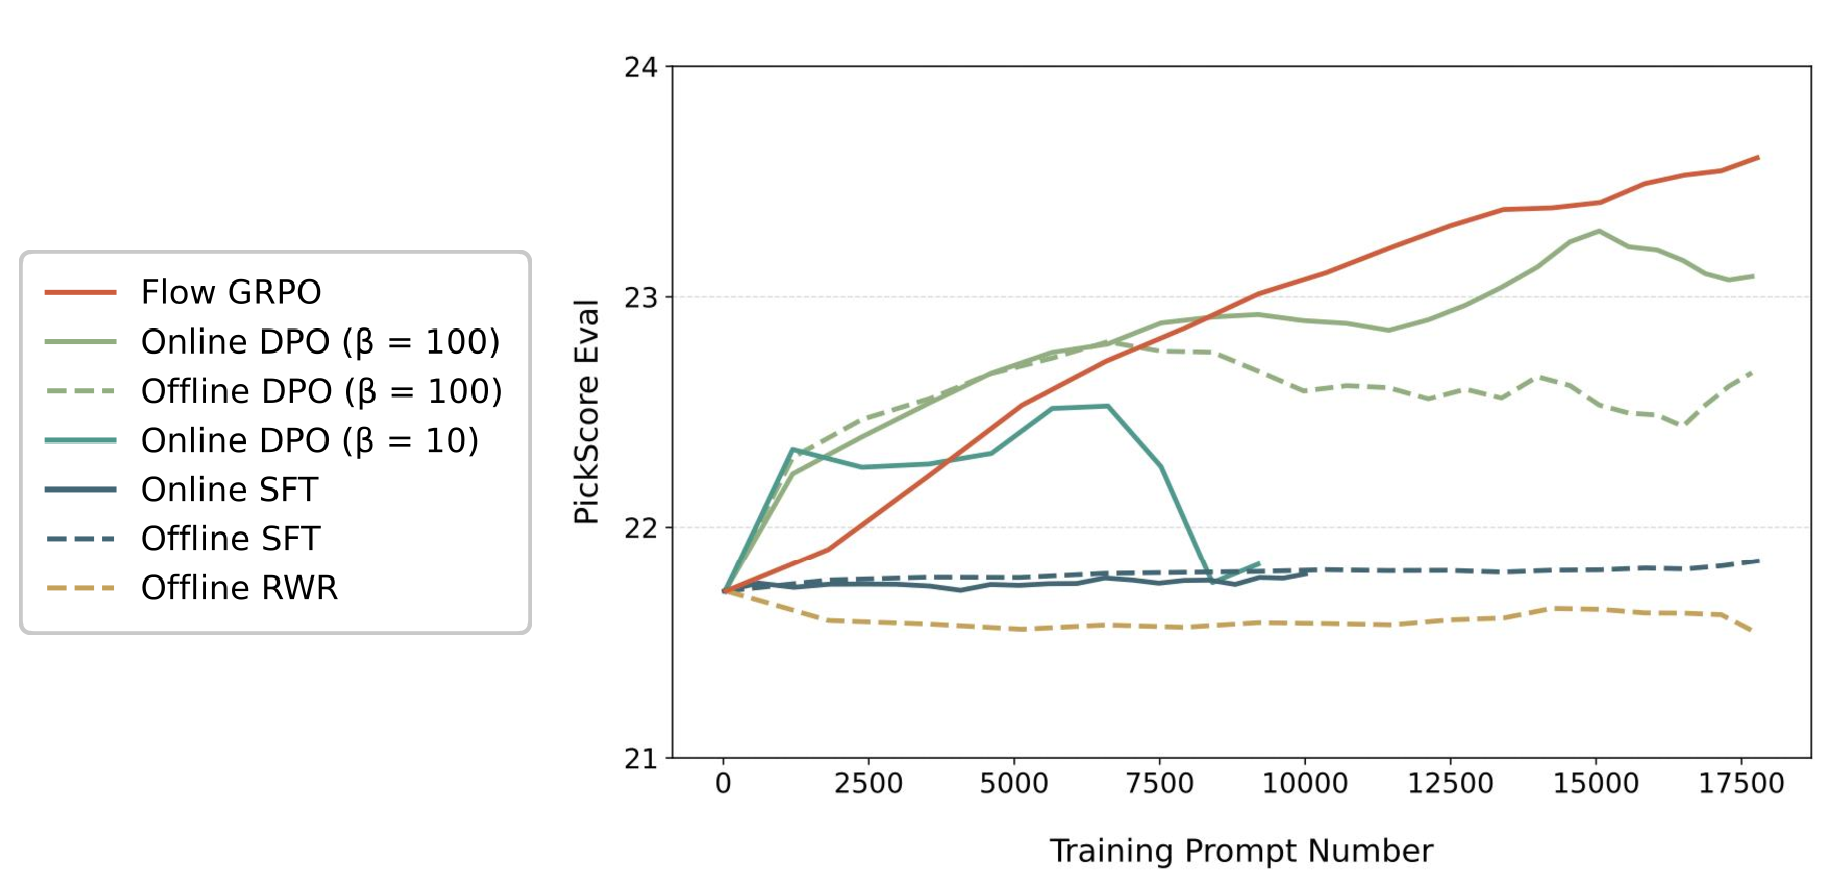
\includegraphics[width=0.9\linewidth]{src/experiments/compare_curve.pdf}
  \end{minipage}
  \begin{minipage}[t]{\textwidth}
    \centering
    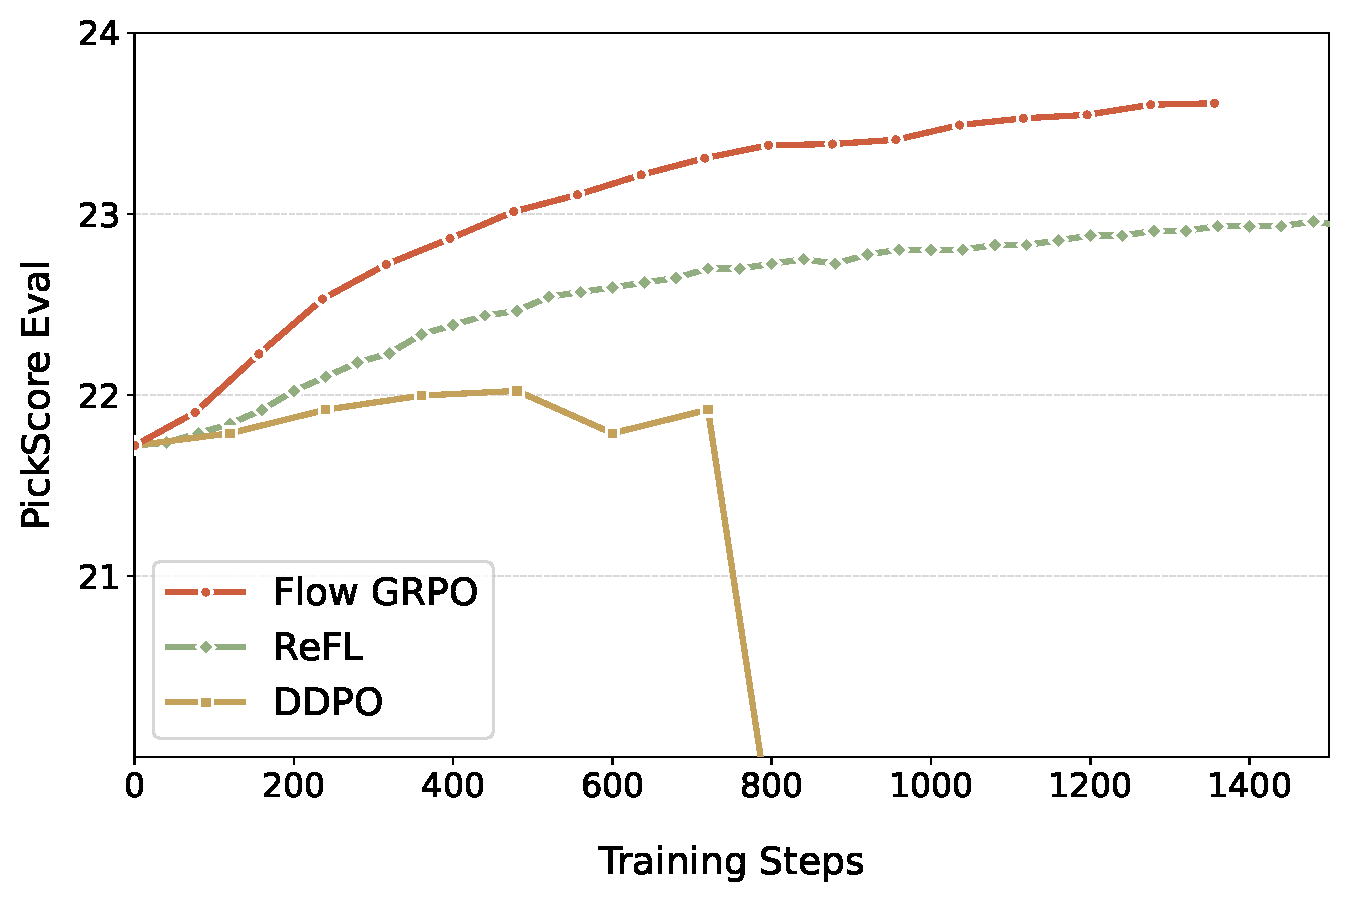
\includegraphics[width=0.6\linewidth]{src/experiments/camera_ready_add/camera_ready_refl.pdf}
  \end{minipage}
    \caption{Comparison of Flow-GRPO and Other Alignment Methods on the Human Preference Alignment task. Since methods like DPO use different tuned batch sizes from Flow-GRPO, we use the number of training prompts on the x-axis for a fair comparison across these methods.
}
  \label{app:fig:compare_curva}
\end{figure}

% \begin{figure}[htbp]
% \centering
% 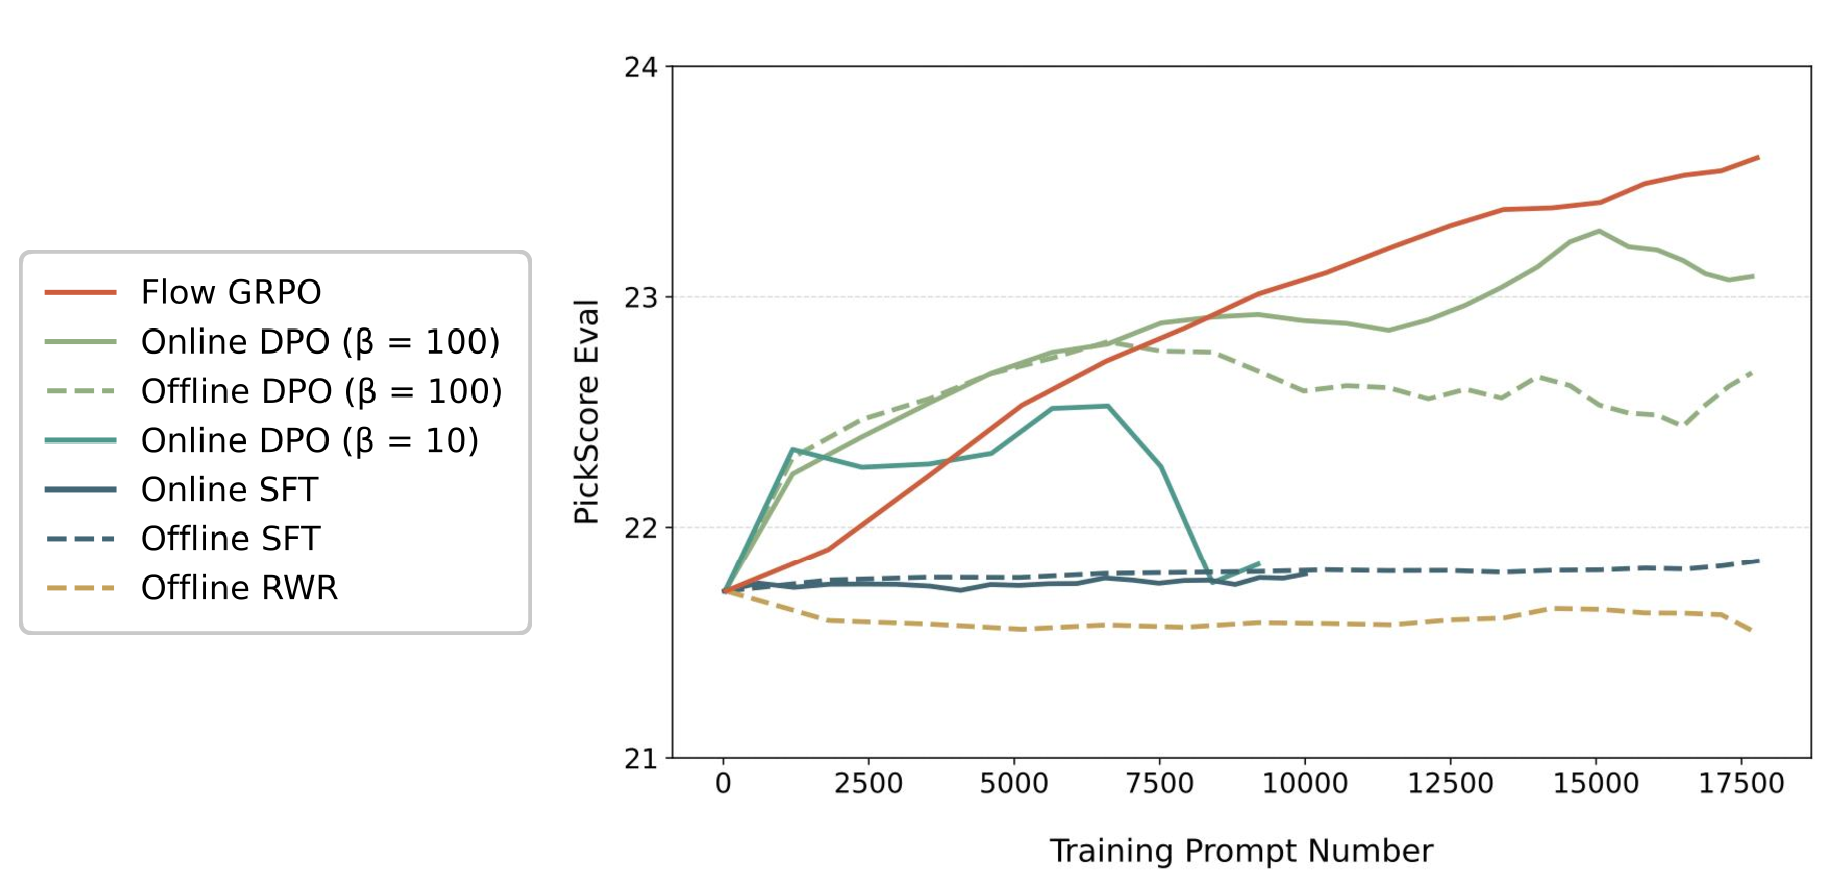
\includegraphics[width=0.9\textwidth]{src/experiments/compare_curve.pdf}
% \caption{Comparison of Flow-GRPO and Other Alignment Methods on the Human Preference Alignment task.
% }
% \label{app:fig:compare_curva}
% \end{figure}

\paragraph{DDPO.} 
DDPO~\cite{ddpo} was originally developed for diffusion-based backbones, so we adapted it to flow-matching models via our ODE-to-SDE conversion. Using SD3.5-M as the base model and PickScore as the reward signal, we track the evaluation reward throughout the entire training process in Figure~\ref{app:fig:compare_curva}. We find that DDPO’s reward increases more slowly than Flow-GRPO’s and eventually collapses in the later stages, whereas Flow-GRPO trains stably and continues to improve consistently over time.

\paragraph{ReFL.}
ReFL~\cite{xu2024imagereward} directly fine-tunes diffusion models by viewing reward model scores as human preference losses and back-propagating gradients to a randomly-picked late timestep $t$.
Following ImageReward~\cite{xu2024imagereward}, we back-propagate gradients to a randomly chosen late timestep $t \in [30, 40]$ during denoising. Figure~\ref{app:fig:compare_curva} shows that GRPO surpasses ReFL when the reward is differentiable, indicating that GRPO maintains strong performance in settings where ReFL applies. More importantly, GRPO does not require differentiable rewards, enabling direct use of state-of-the-art Vision-Language Models (VLMs) as reward providers. This offers two key advantages:

\begin{itemize}[leftmargin=10pt]
\item \textbf{Sophisticated, General-Purpose Rewards:} VLMs can conduct human-like evaluations through a structured reasoning process. Given a prompt, a VLM can decompose it into key criteria, reason step by step to verify each aspect in the generated image, and then provide a comprehensive overall score. This enables a single, unified reward model to handle diverse tasks, from text-to-image generation to complex instruction-based image editing.

\item \textbf{Future-Proof and Cost-Free Upgrades:} The field of VLMs is advancing at a breathtaking pace. By using a VLM as the reward source, our framework automatically benefits from these improvements. As VLMs become more capable, the reward model becomes stronger without any additional training data or computational cost.
\end{itemize}


\paragraph{ORW.}
ORW~\cite{fan2025online} is an online reward-weighted regression method that guides the model to prioritize high-reward regions. Unlike KL regularization, it employs Wasserstein-2 regularization to prevent policy collapse and maintain diversity.
To ensure a fair comparison, we adopt the same experimental setup as in our Human Preference Alignment task.
For ORW, we set $\beta = 0.5$ and $\alpha = 1$ (lower values led to unstable training). The $\text{steps\_per\_epoch}$ parameter, which controls how frequently the data-collecting policy is updated, was chosen from ${20, 40, 100, 400}$ based on best performance.
Table~\ref{tab:sd35_flowgrpo_orw} reports reward scores on the test set across training steps.
Following ORW’s Table 1, we randomly sampled 50 DrawBench prompts and generated 64 images per prompt to compute CLIP and Diversity scores.
As shown in Table~\ref{tab:clip_diversity_scores}, Flow-GRPO outperforms ORW on both metrics.

\begin{table}[h]
\centering
\small
\caption{Reward scores on the test set over training steps.}
\begin{tabular}{lccccc}
\toprule
\textbf{Method} & \textbf{Step 0} & \textbf{Step 240} & \textbf{Step 480} & \textbf{Step 720} & \textbf{Step 960} \\
\midrule
SD3.5-M + ORW & 28.79 & 29.05 & 29.15 & 27.58 & 23.05 \\
\textbf{SD3.5-M + Flow-GRPO} & 28.79 & \textbf{29.10} & \textbf{29.17} & \textbf{29.51} & \textbf{29.89} \\
\bottomrule
\end{tabular}
\label{tab:sd35_flowgrpo_orw}
\end{table}

\begin{table}[h]
\centering
\small
\setlength{\tabcolsep}{24pt}
\caption{Comparison of CLIP and diversity scores across different fine-tuning methods.}
\begin{tabular}{lcc}
\toprule
\textbf{Method} & \textbf{CLIP Score} $\uparrow$ & \textbf{Diversity Score} $\uparrow$ \\
\midrule
SD3.5-M & 27.99 & 0.96 \\
SD3.5-M + ORW & 28.40 & 0.97 \\
\textbf{SD3.5-M + Flow-GRPO} & \textbf{30.18} & \textbf{1.02} \\
\bottomrule
\end{tabular}
\label{tab:clip_diversity_scores}
\end{table}



\subsection{Effect of Denoising Reduction}\label{app:subsec:noising_reduction}
We show the extended Denoising Reduction ablations of Visual Text Rendering and Human Preference Alignment tasks in Figure~\ref{app:fig:exp2_ablation_step}.
\begin{figure}[htbp]
  \centering
  \begin{minipage}[t]{0.48\textwidth}
    \centering
    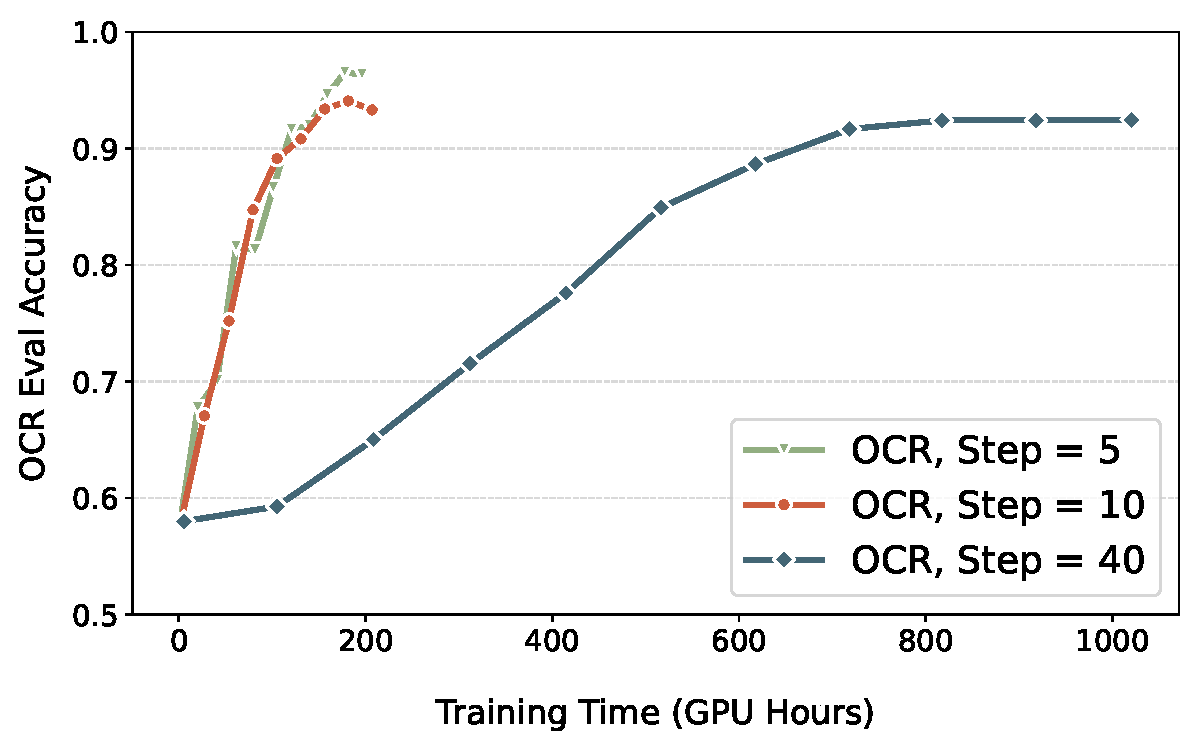
\includegraphics[width=\linewidth]{src/experiments/ablation_step/exp2_ocr_ablation_step.pdf}
    \caption*{\footnotesize (a) Visual Text Rendering}
  \end{minipage}
  \begin{minipage}[t]{0.48\textwidth}
    \centering
    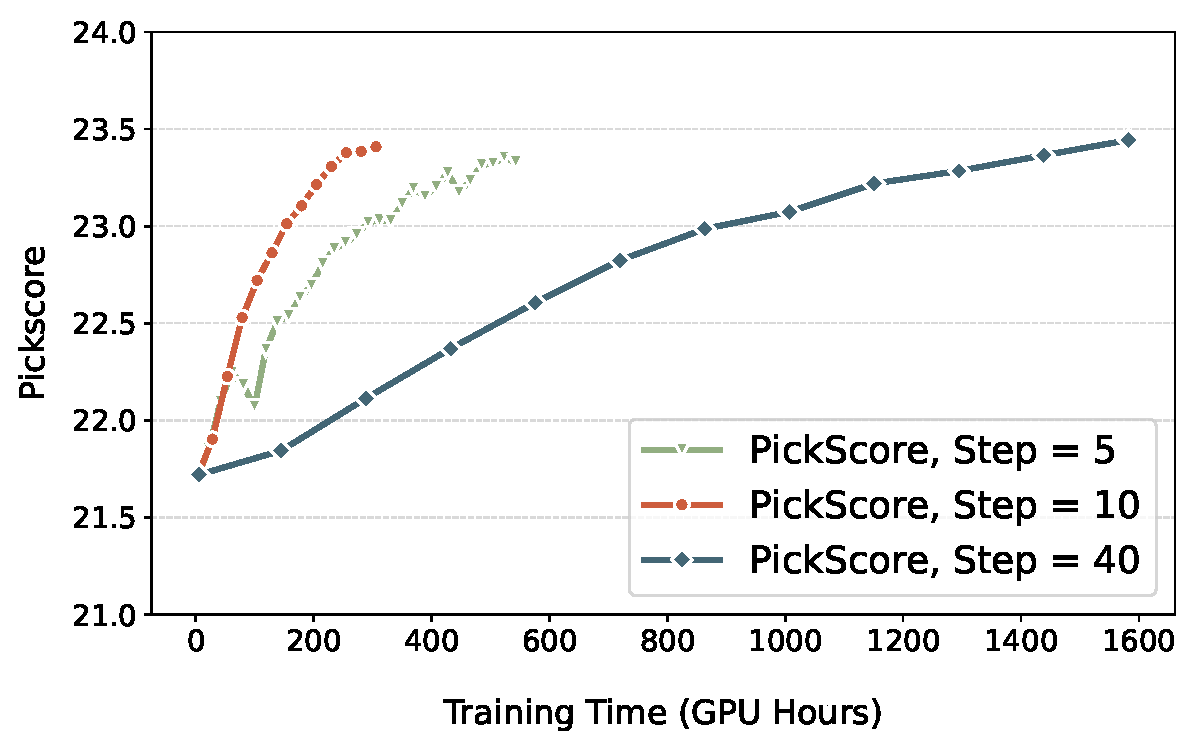
\includegraphics[width=\linewidth]{src/experiments/ablation_step/exp2_pickscore_ablation_step.pdf}
    \vspace{-1.5em}
    \caption*{\footnotesize (b) Human Preference Alignment}
  \end{minipage}
    \caption{Effect of Denoising Reduction}
  \label{app:fig:exp2_ablation_step}
\end{figure}

\subsection{Effect of Initial Noise}\label{app:subsec:initial_noise}
We initialize each rollout with difference random noise to increase exploratory diversity during RL training. We perform an additioanl ablation to confirm this claim. With SD3.5-M as the base model and PickScore as the reward, we compare Flow-GRPO with different initial noise against Flow-GRPO with the same initial noise. Figure~\ref{app:fig:effect_initial_noise} shows the variant with different noise consistently achieved high rewards during the training process. 

\newpage

% \begin{figure}[htbp]
% \centering
% 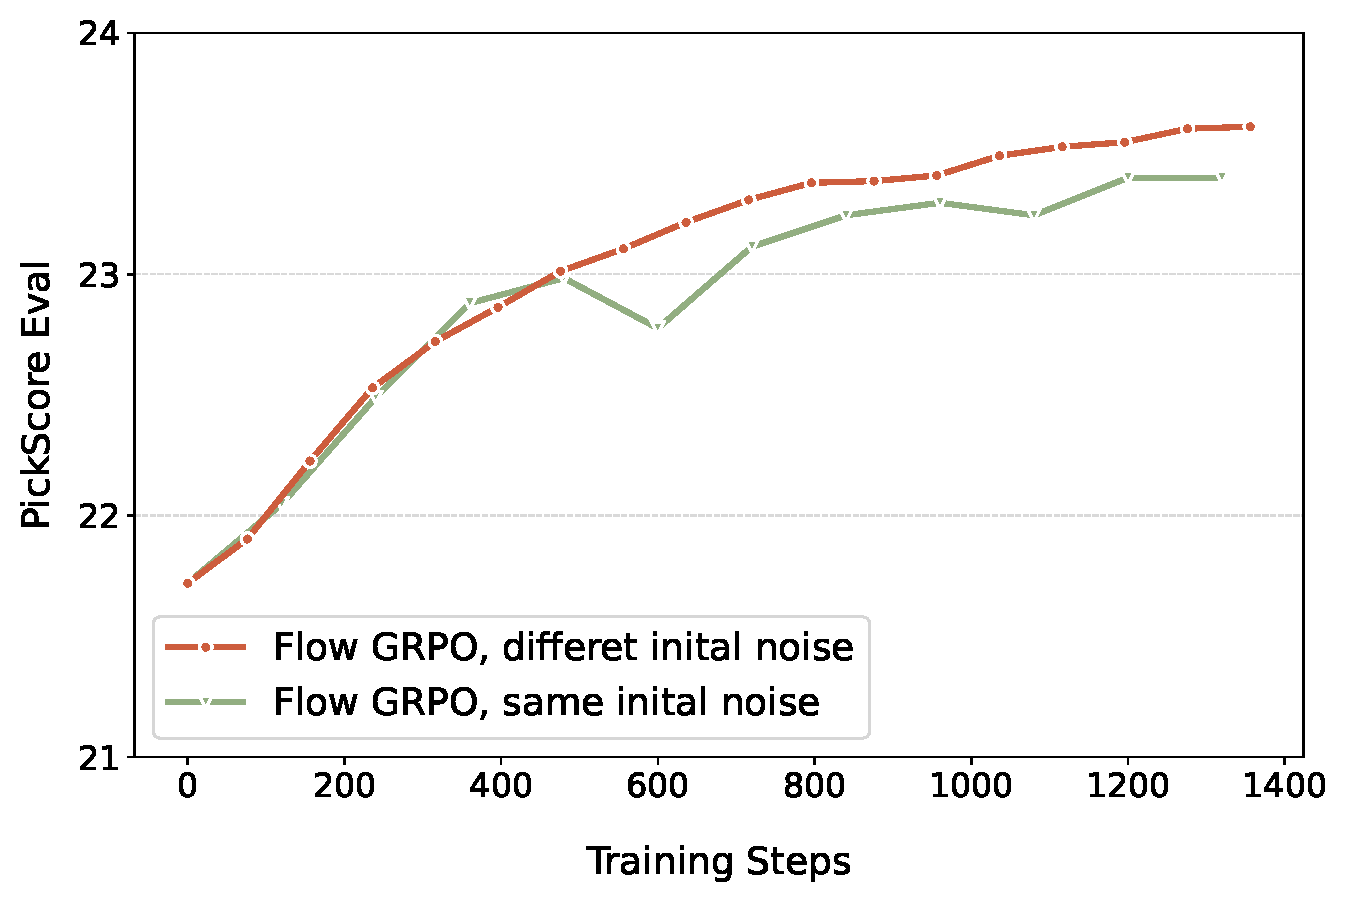
\includegraphics[width=0.6\textwidth]{src/experiments/camera_ready_add/camera_ready_noise.pdf}
% \caption{Effect of Initial Noise.
% }
% \label{app:fig:effect_initial_noise}
% \end{figure}

\begin{figure}[htbp]
  \centering
  \begin{minipage}[t]{0.48\textwidth}
    \centering
    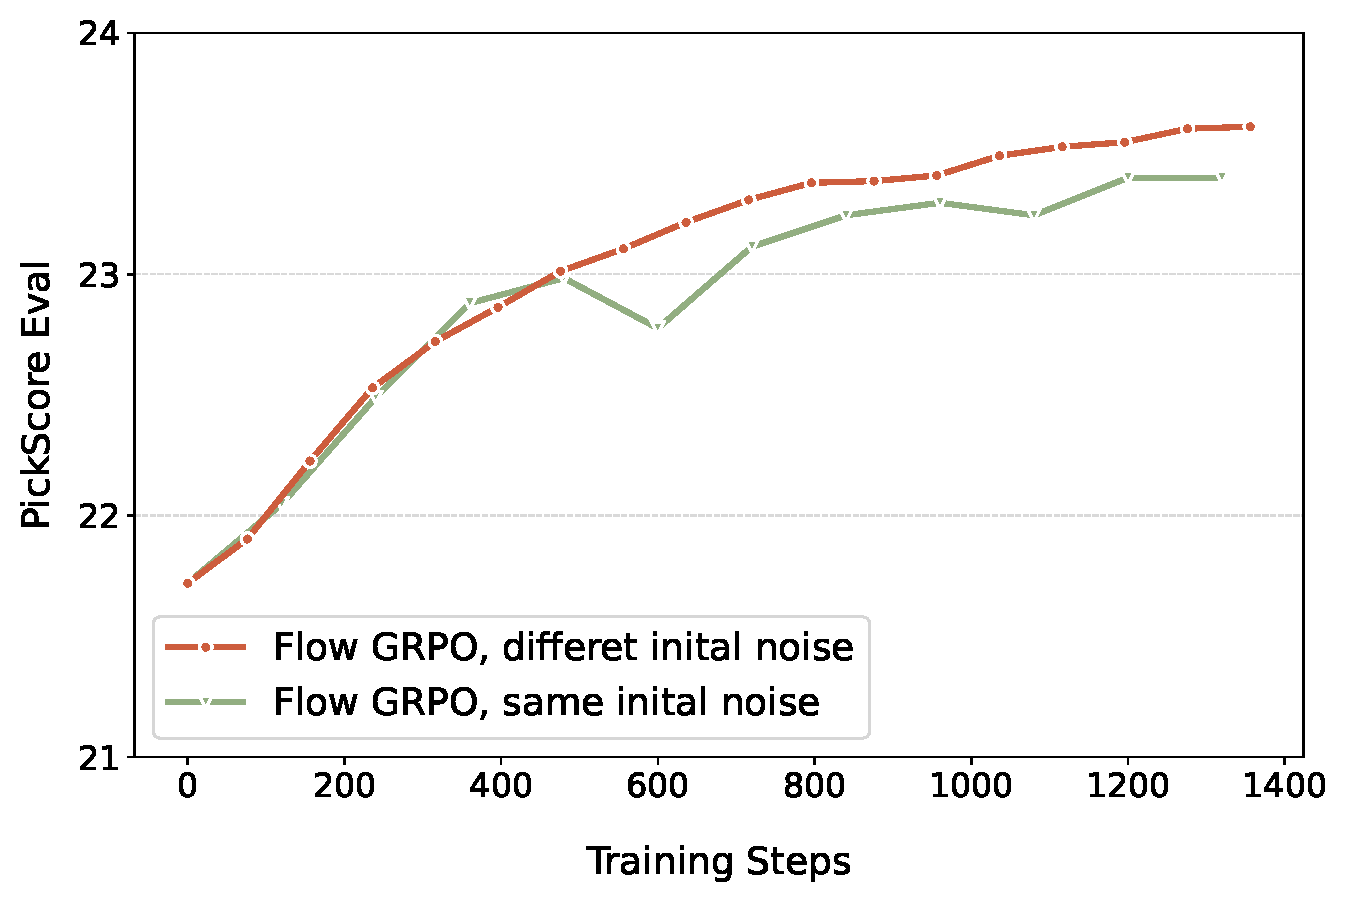
\includegraphics[width=\linewidth]{src/experiments/camera_ready_add/camera_ready_noise.pdf}
    \caption{Effect of Initial Noise}
    \label{app:fig:effect_initial_noise}
  \end{minipage}
  \begin{minipage}[t]{0.48\textwidth}
    \centering
    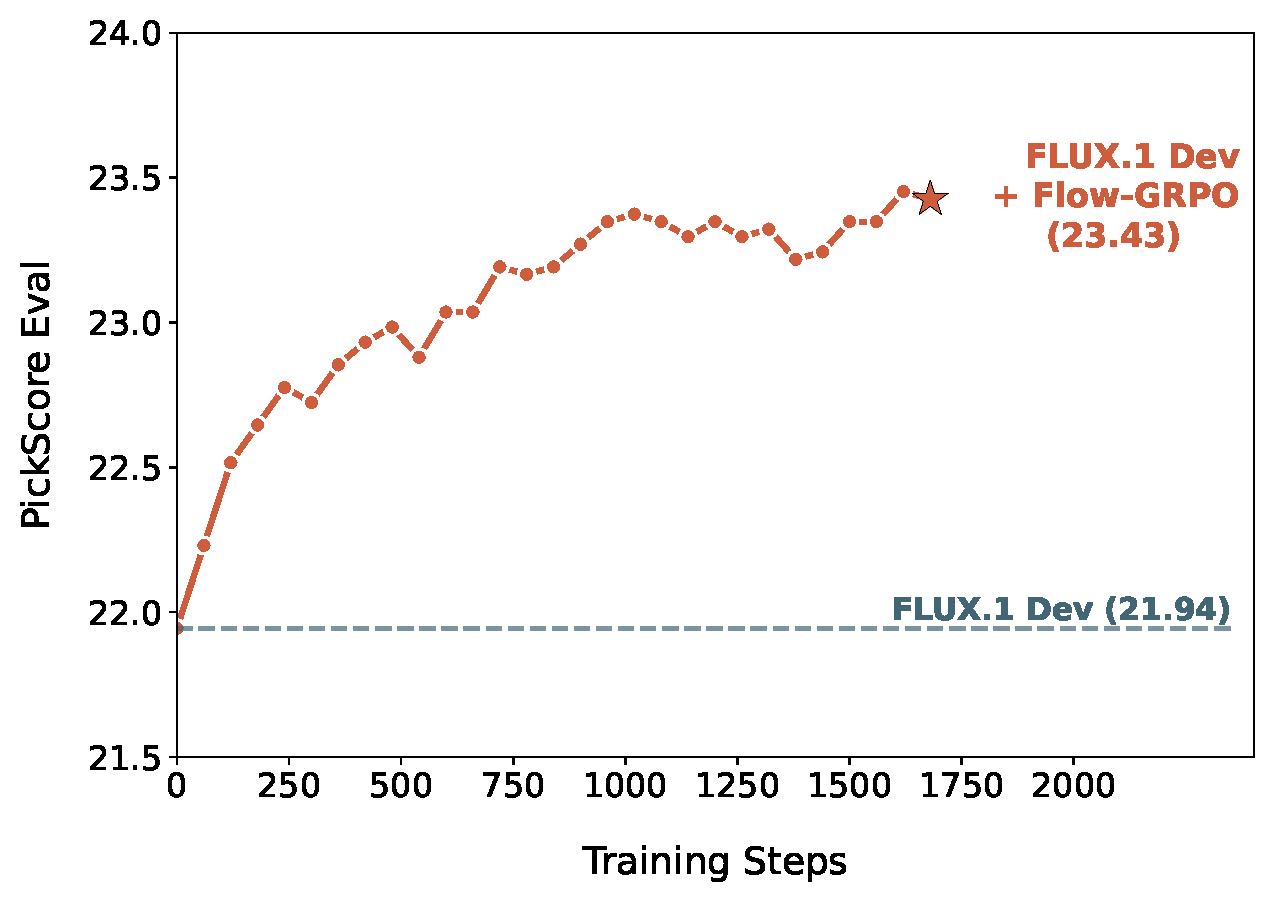
\includegraphics[width=\linewidth]{src/experiments/camera_ready_add/camera_ready_flux.pdf}
    \caption{Additional Results on FLUX.1-Dev}
    \label{app:fig:effect_flux}
  \end{minipage}
\end{figure}


\subsection{Additional Results on FLUX.1-Dev}\label{app:subsec:flux}
We run Flow-GRPO on FLUX.1-Dev~\cite{flux2024} using PickScore as the reward signal. The reward curve rises steadily throughout training without noticeable reward hacking. Figure~\ref{app:fig:effect_flux} shows the reward values over the training process, and Table~\ref{tab:flux_flowgrpo_results} compares FLUX.1-Dev with FLUX.1-Dev + Flow-GRPO on DrawBench.

\begin{table}[h]
\centering
\small
\caption{Comparison of FLUX.1-Dev and Flow-GRPO fine-tuned models.}
\begin{tabular}{lccccc}
\toprule
\textbf{Model} & \textbf{Aesthetic} & \textbf{DeQA} & \textbf{ImageReward} & \textbf{PickScore} & \textbf{UnifiedReward} \\
\midrule
FLUX.1-Dev & 5.71 & 4.31 & 0.85 & 22.62 & 3.65 \\
FLUX.1-Dev + Flow-GRPO & 6.02 & 4.24 & 1.32 & 23.97 & 3.81 \\
\bottomrule
\end{tabular}
\label{tab:flux_flowgrpo_results}
\end{table}

% \vspace{-1em}

% \begin{figure}[h]
% \centering
% 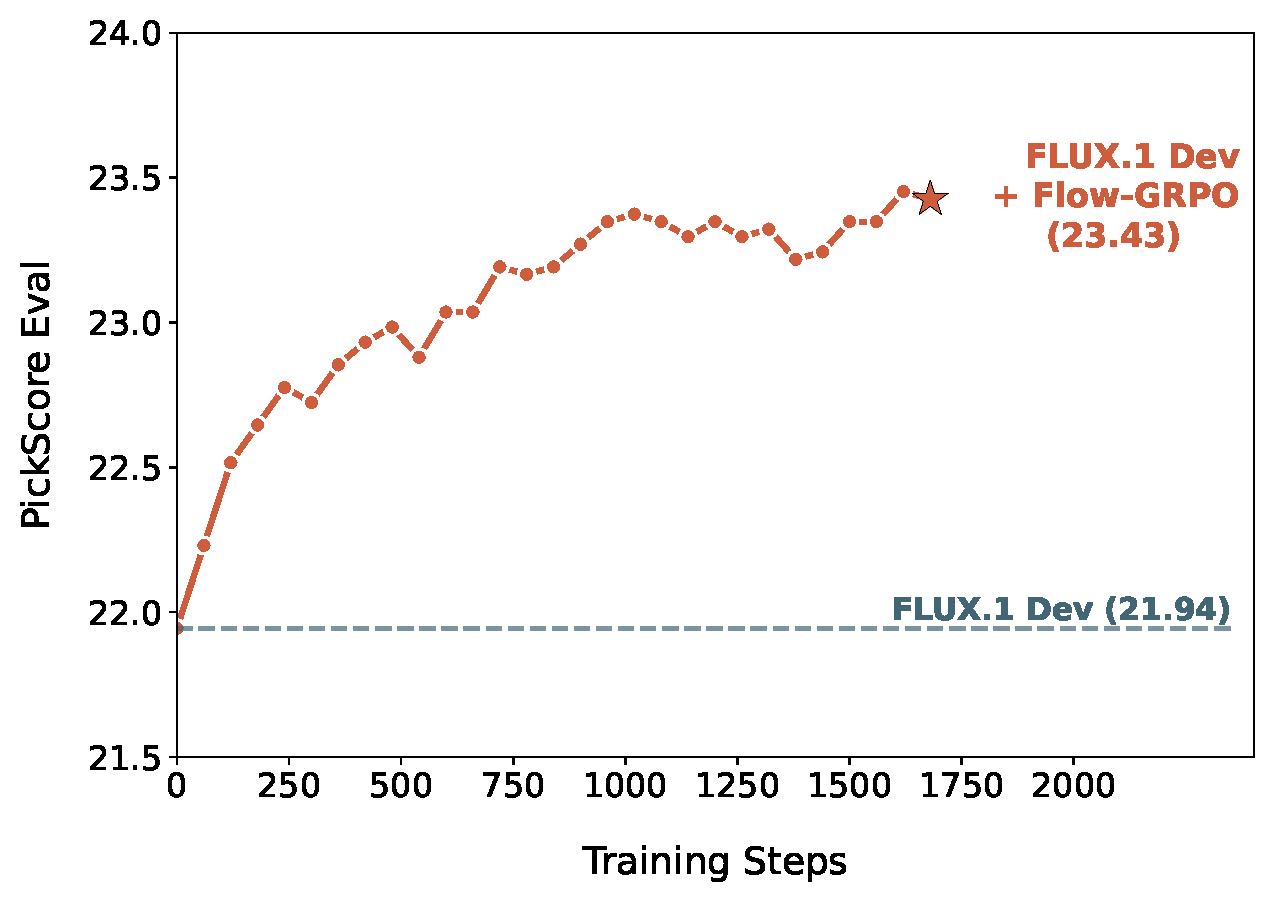
\includegraphics[width=0.6\textwidth]{src/experiments/camera_ready_add/camera_ready_flux.pdf}
% \caption{Additional Results on FLUX.1-Dev
% }
% \label{app:fig:effect_flux}
% \end{figure}

\subsection{Learning Curves with or without KL}\label{app:subsec:training_curve_kl}
Figure~\ref{app:fig:exp3_ablation_kl} shows learning curves for three tasks, with and without KL. These results emphasize that KL regularization is not empirically equivalent to early stopping. Adding appropriate KL can achieve the same high reward as the KL-free version and maintain image quality, though it requires longer training.
\begin{figure}[htbp]
  \centering
  \begin{minipage}[t]{0.48\textwidth}
    \centering
    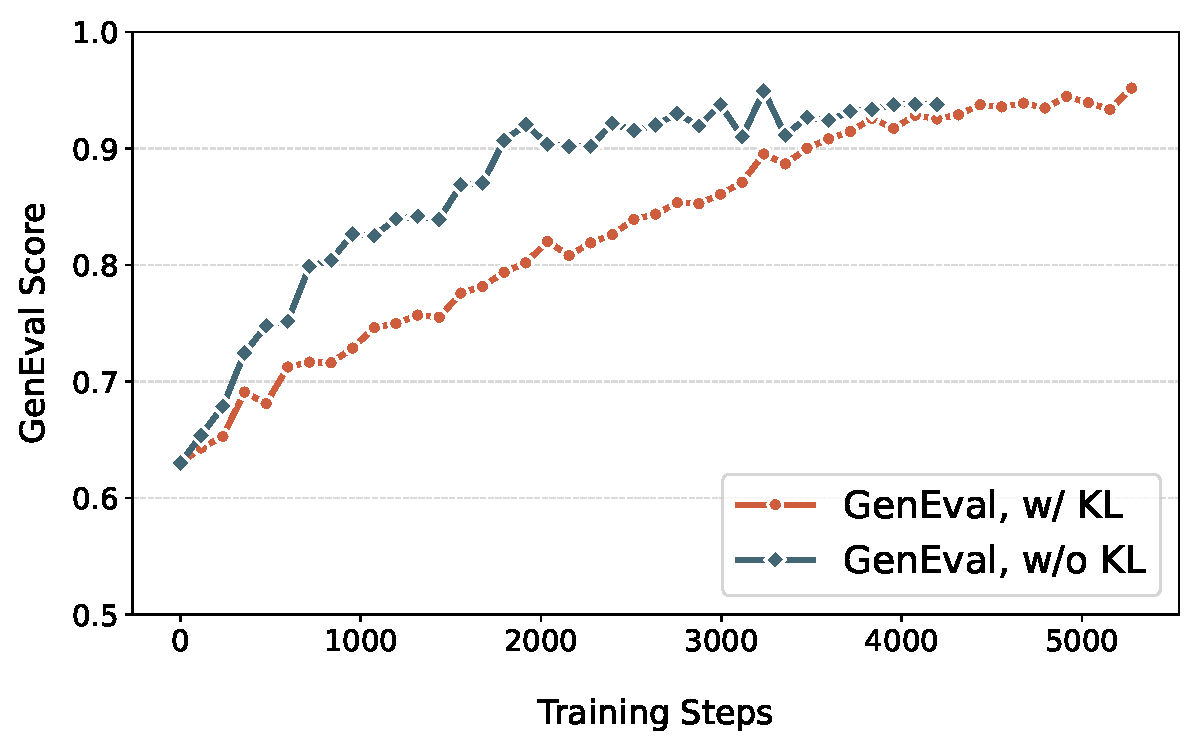
\includegraphics[width=\linewidth]{src/experiments/ablation_kl/exp3_geneval_ablation_kl.pdf}
    \vspace{-1.5em}
    \caption*{\footnotesize (a) Compositional Image Generation}
  \end{minipage}
  \hfill
  \begin{minipage}[t]{0.48\textwidth}
    \centering
    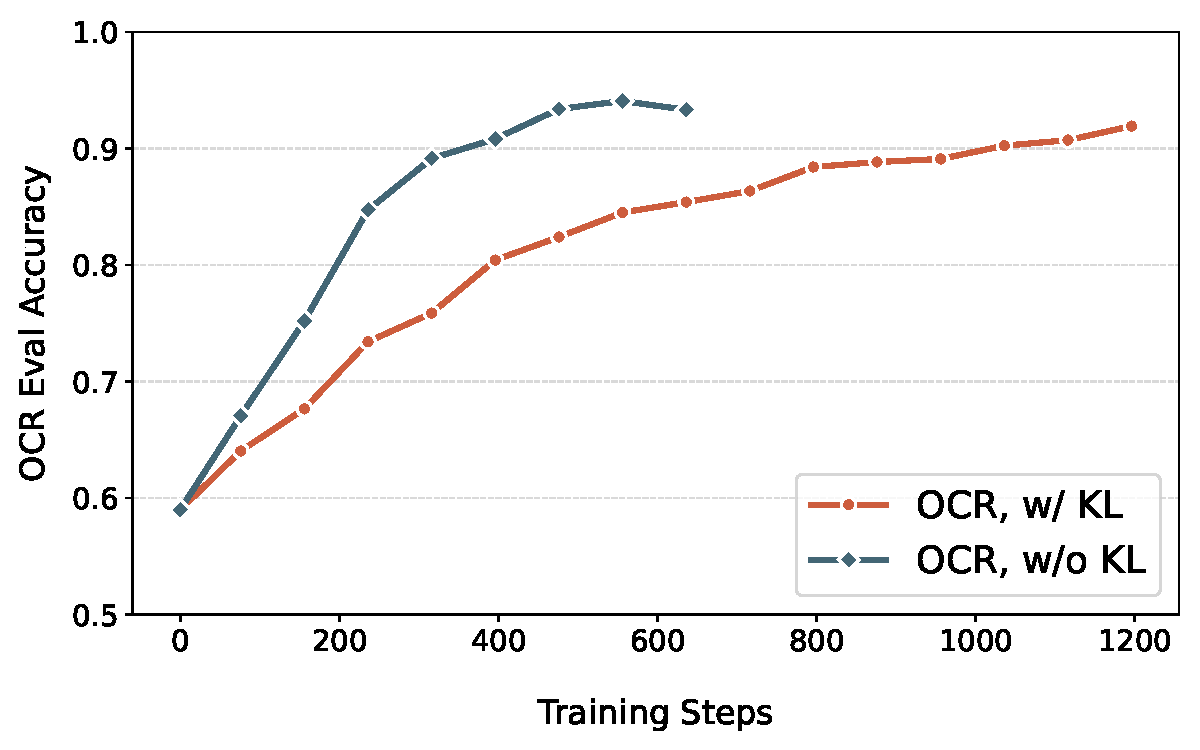
\includegraphics[width=\linewidth]{src/experiments/ablation_kl/exp3_ocr_ablation_kl.pdf}
    \vspace{-1.5em}
    \caption*{\footnotesize (b) Visual Text Rendering}
  \end{minipage}
  \vspace{1.5em}

  \begin{minipage}[t]{0.48\textwidth}
    \centering
    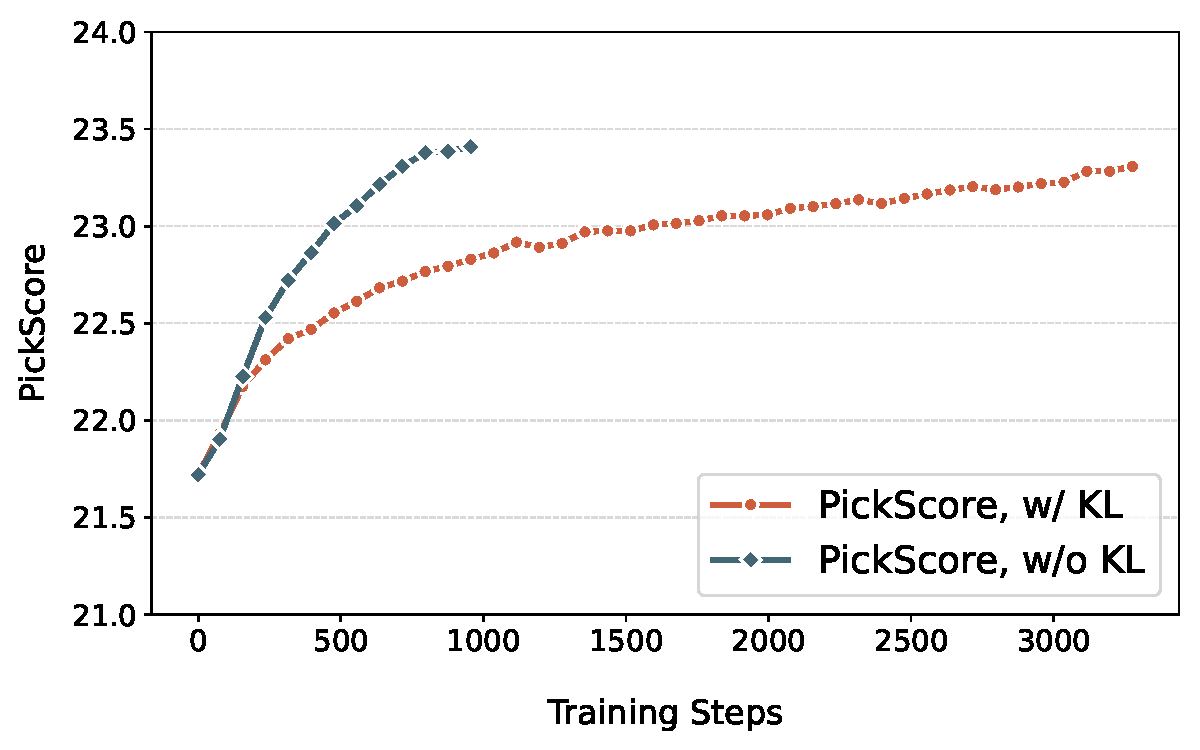
\includegraphics[width=\linewidth]{src/experiments/ablation_kl/exp3_pickscore_ablation_kl.pdf}
    \vspace{-1.5em}
    \caption*{\footnotesize (c) Human Preference Alignment}
  \end{minipage}
  \caption{Learning Curves with and without KL. KL penalty slows early training yet effectively suppresses reward hacking.}
  \label{app:fig:exp3_ablation_kl}
\end{figure}



\subsection{Additional Qualitative Results}\label{app:subsec:qualitative_results}
Figures~\ref{app:fig:add_qualitative_result_geneval}, \ref{app:fig:add_qualitative_result_ocr} \& \ref{app:fig:add_qualitative_result_pickscore} qualitatively compare SD3.5-M with its Flow-GRPO enhanced versions (with and without KL regularization) using GenEval, OCR and PickScore rewards, respectively. Flow-GRPO with KL regularization improves the target capability while maintaining image quality and minimizing reward-hacking. Conversely, removing the KL constraint significantly degrades image quality and diversity.

\begin{figure}[htbp]
\centering
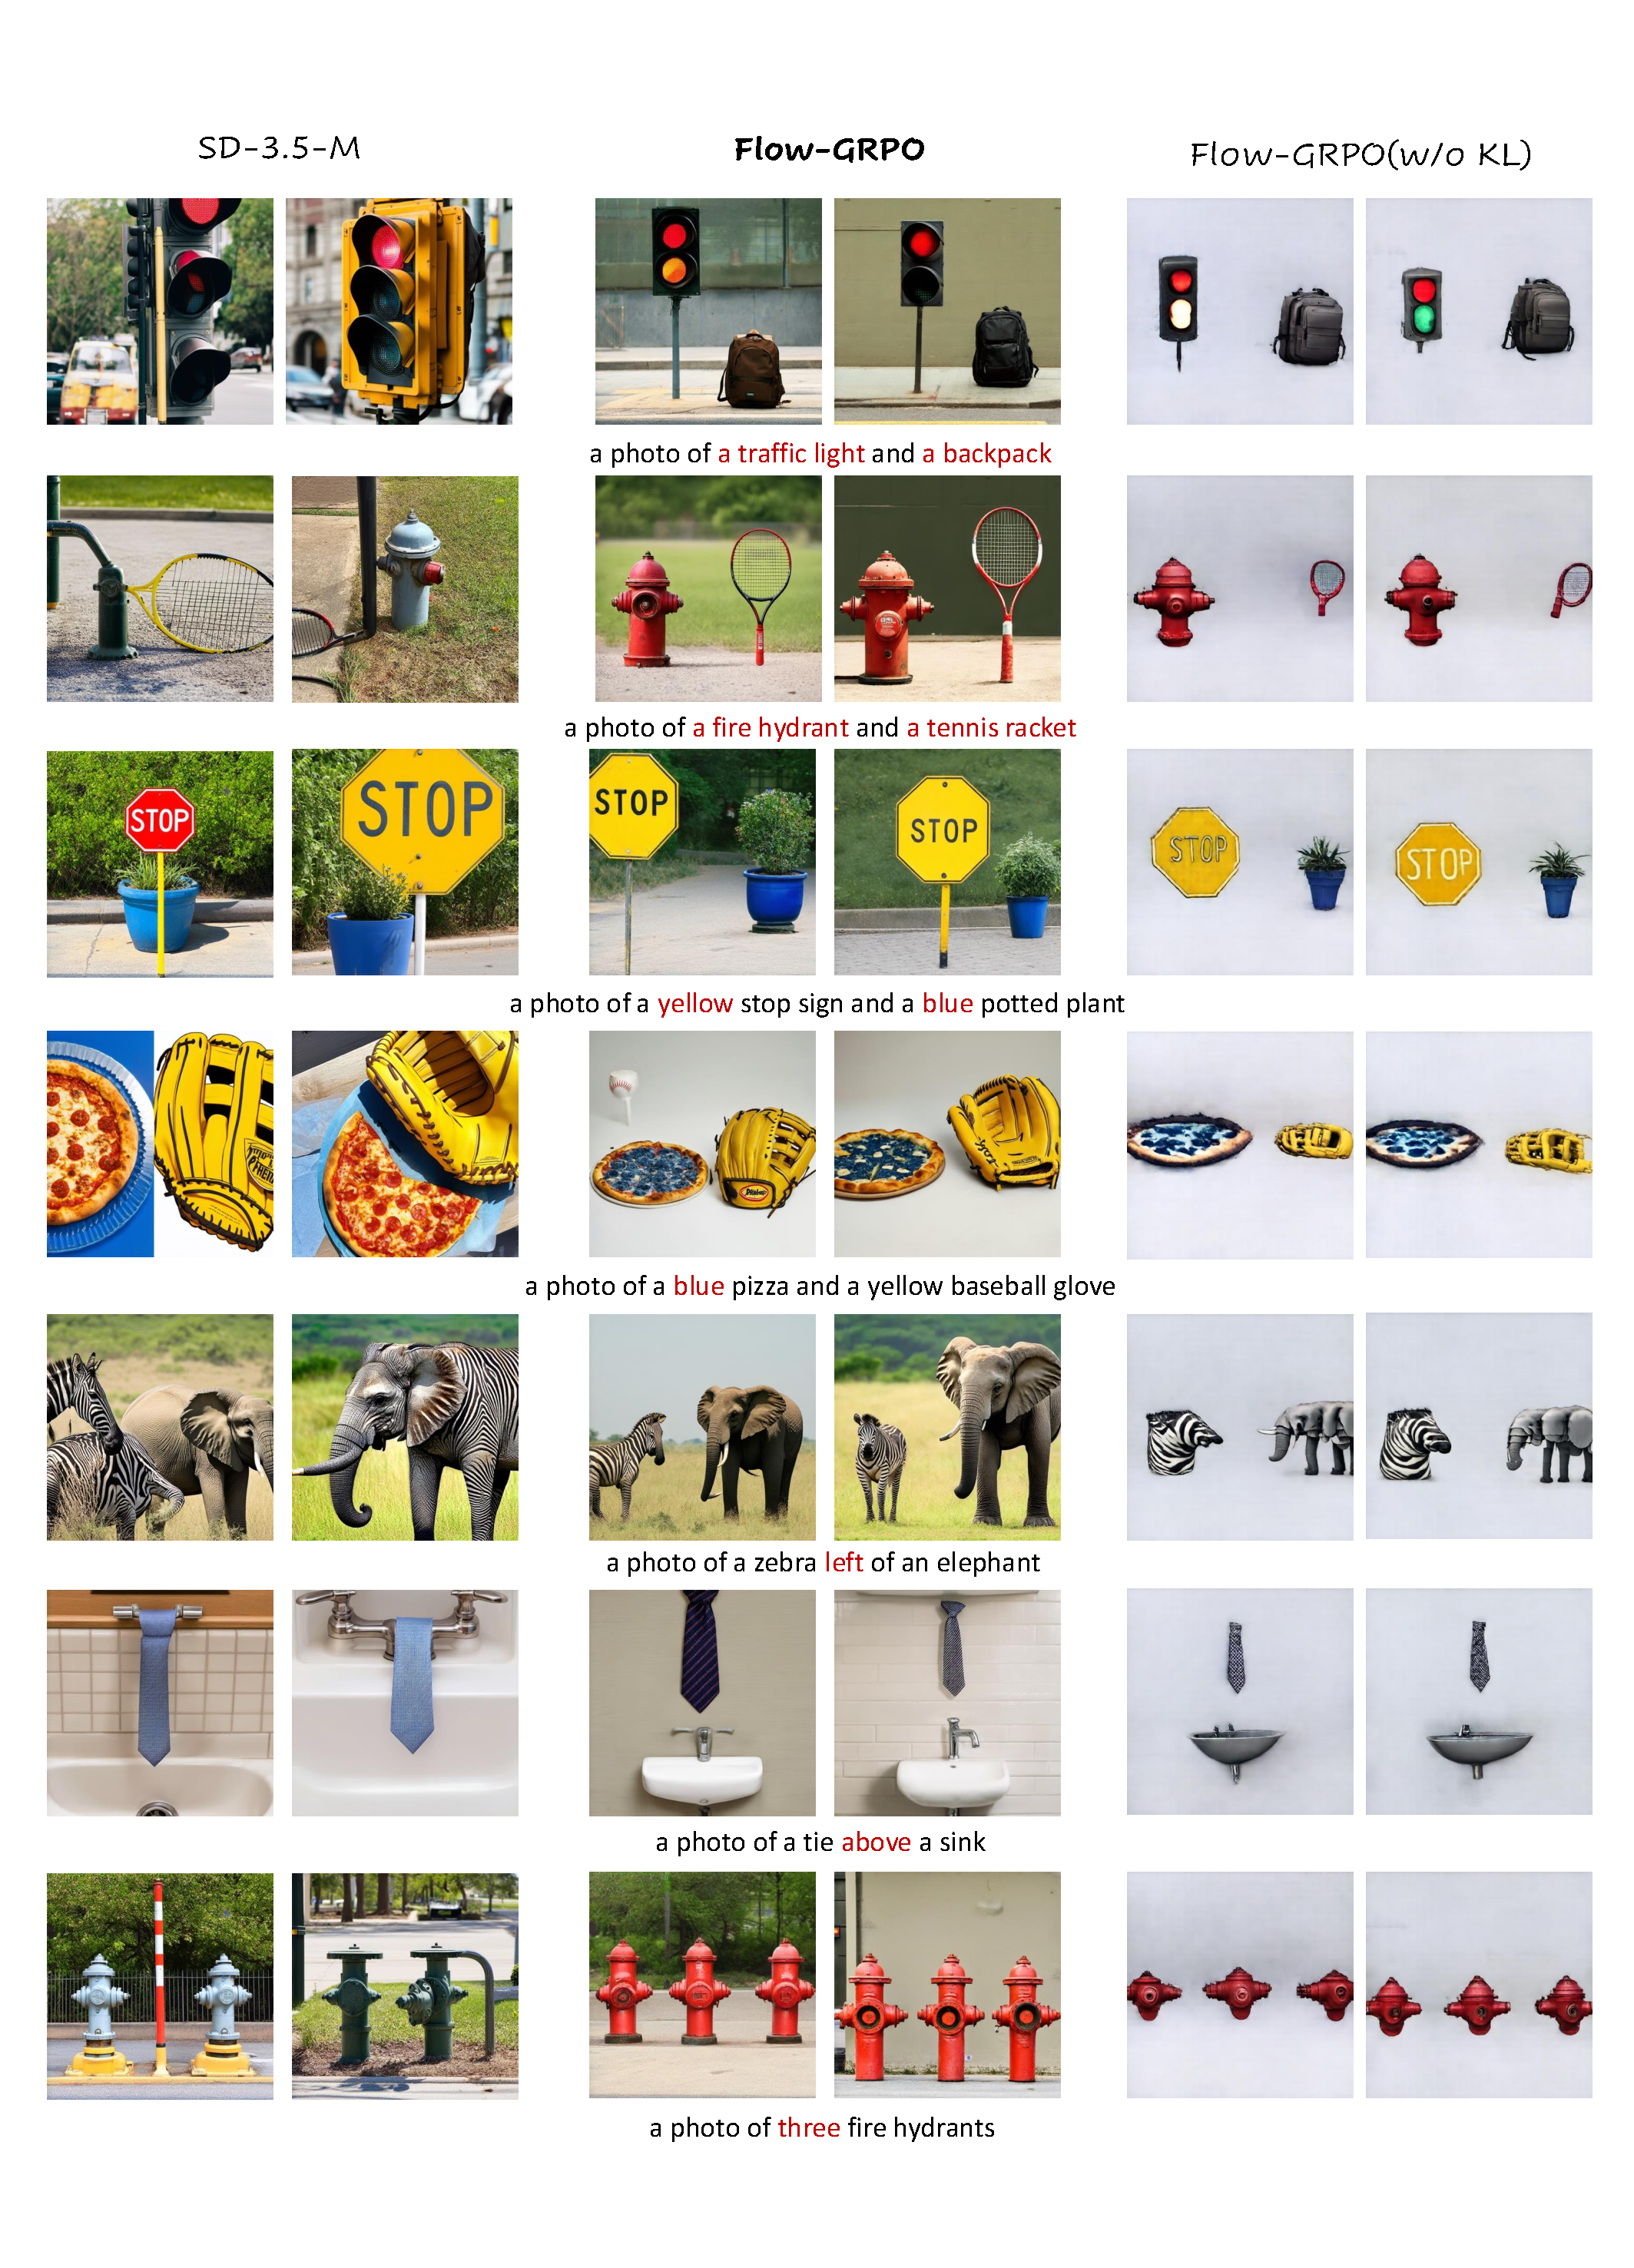
\includegraphics[width=\textwidth]{src/experiments/more_results_geneval.pdf}
\caption{Additional Qualitative comparison between the SD3.5-M and SD3.5-M + Flow-GRPO trained with \textbf{GenEval} reward.
}
\label{app:fig:add_qualitative_result_geneval}
\end{figure}


\begin{figure}[htbp]
\centering
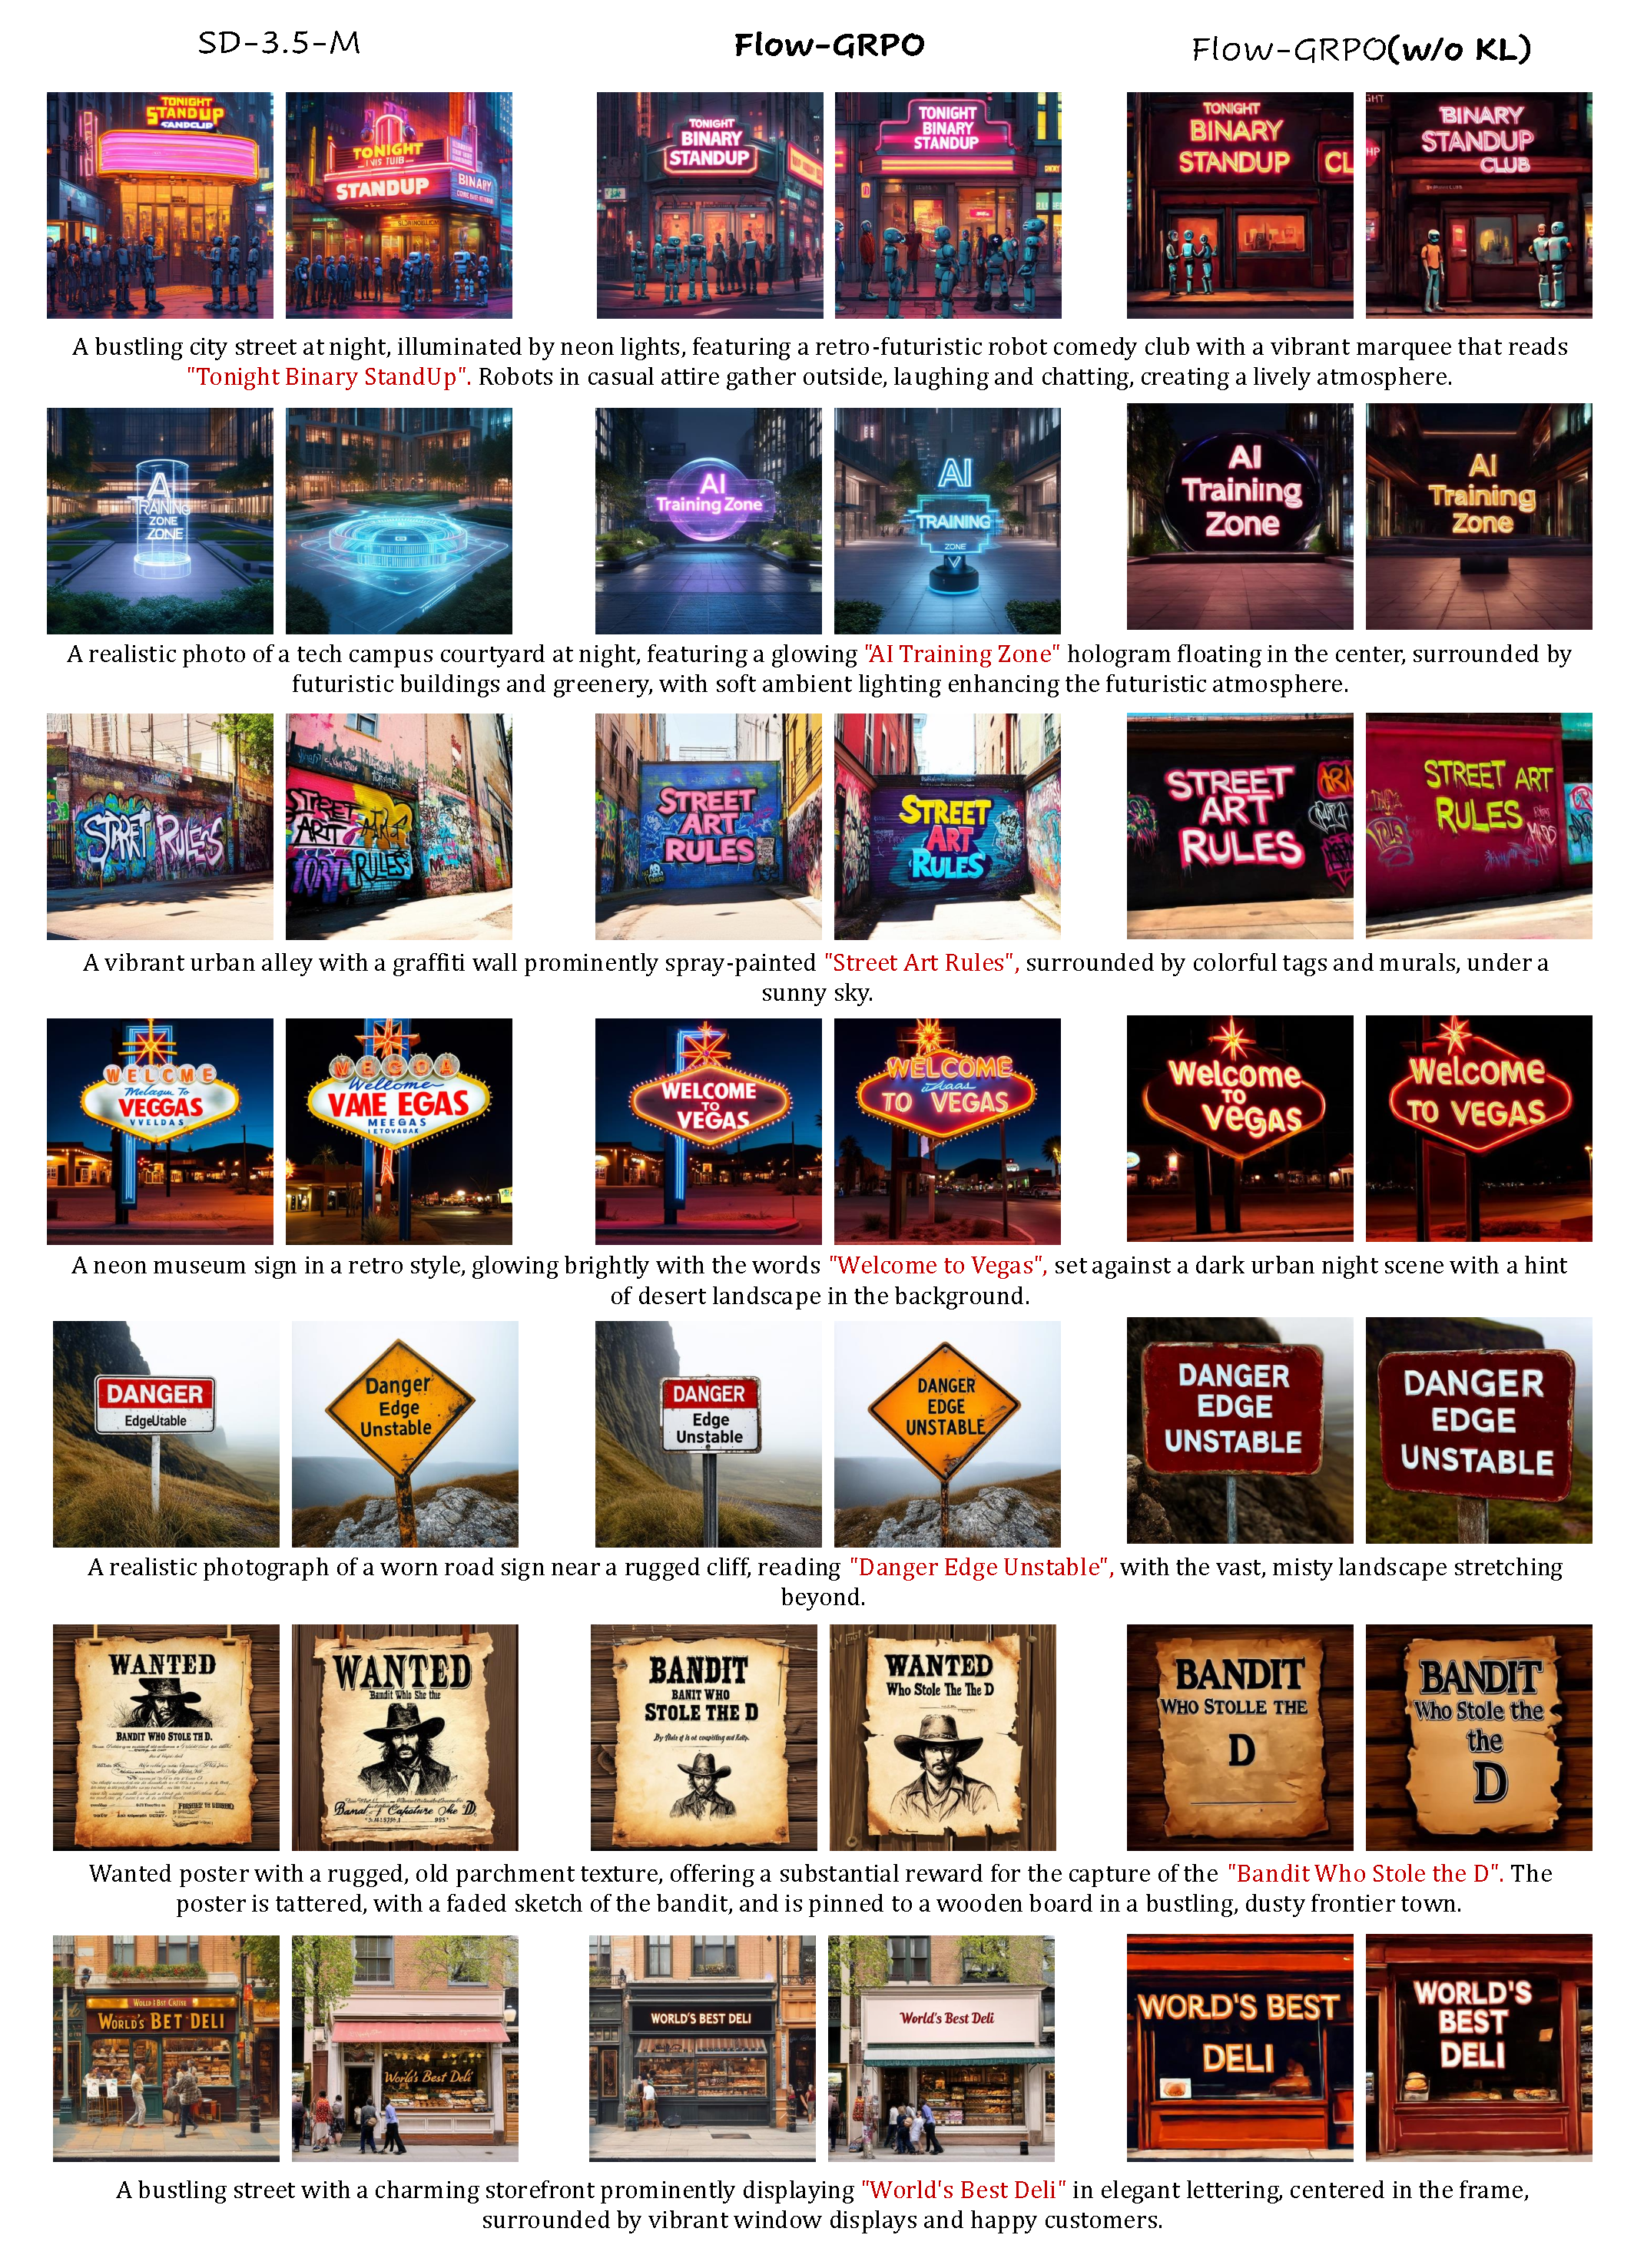
\includegraphics[width=\textwidth]{src/experiments/more_results_ocr.pdf}
\caption{Additional Qualitative comparison between the SD3.5-M and SD3.5-M + Flow-GRPO trained with \textbf{OCR} reward.
}
\label{app:fig:add_qualitative_result_ocr}
\end{figure}

\begin{figure}[htbp]
\centering
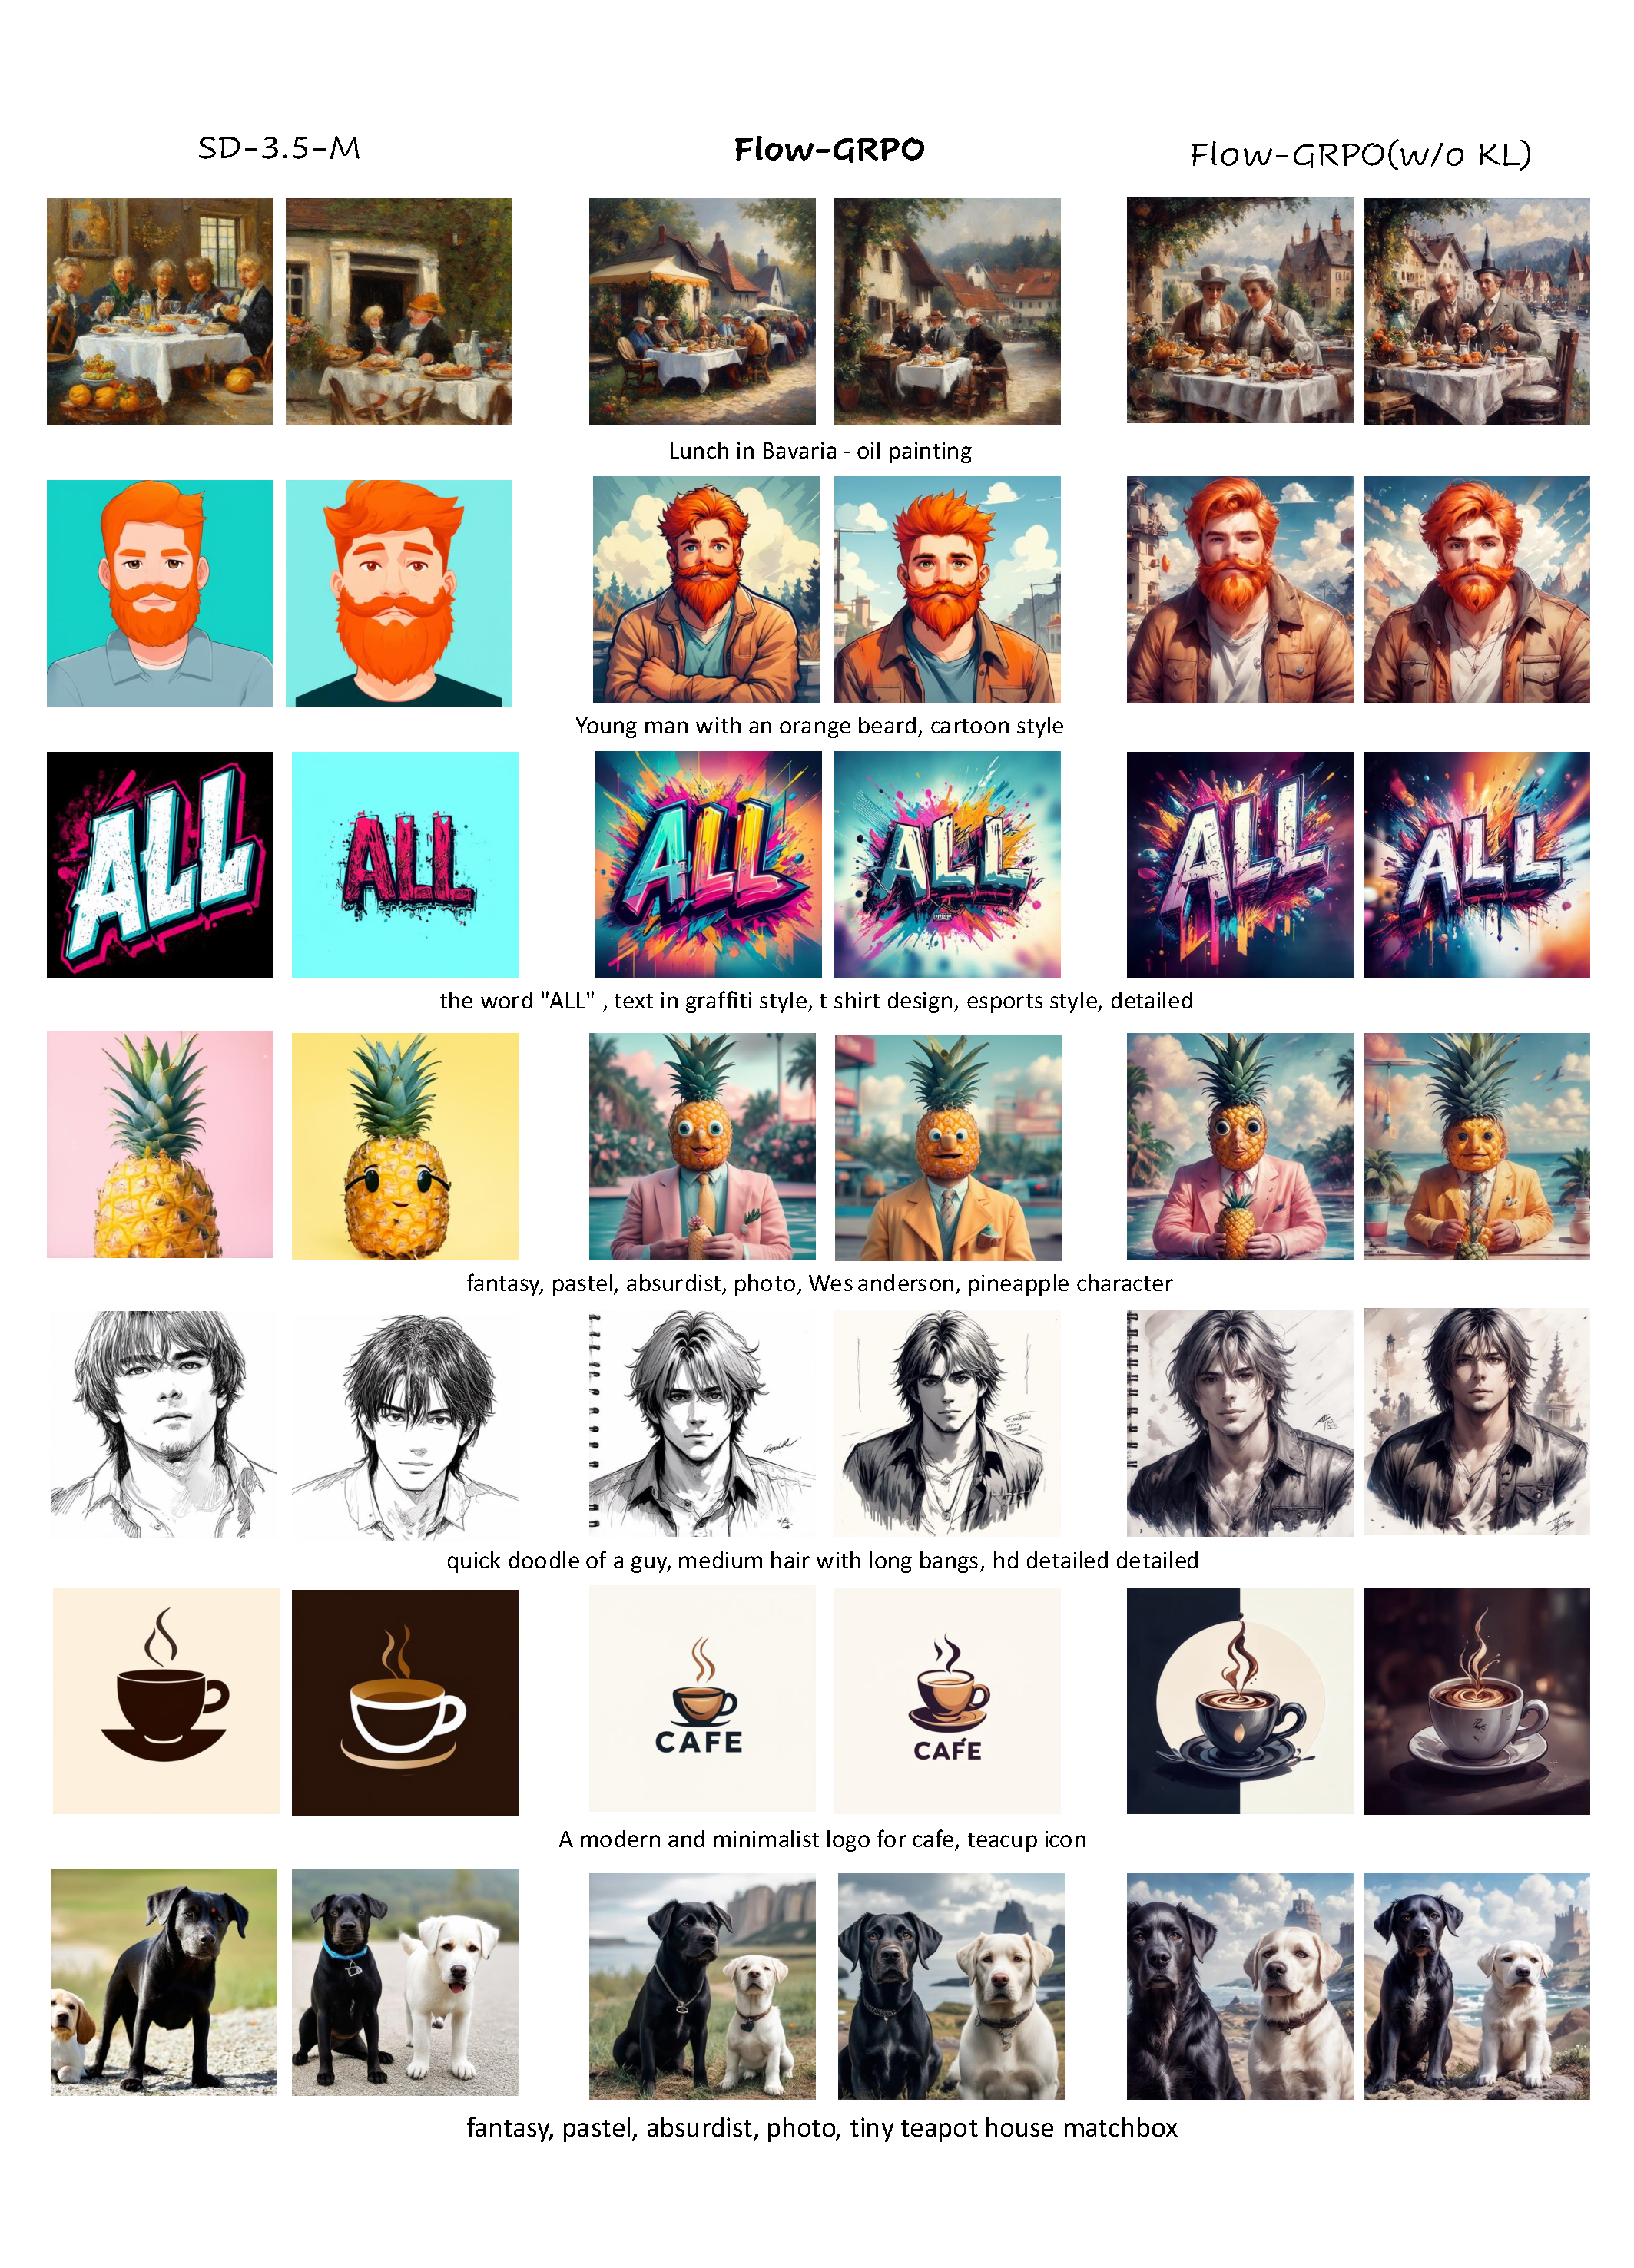
\includegraphics[width=\textwidth]{src/experiments/more_results_pickscore.pdf}
\caption{Additional Qualitative comparison between the SD3.5-M and SD3.5-M + Flow-GRPO trained with \textbf{PickScore} reward.
}
\label{app:fig:add_qualitative_result_pickscore}
\end{figure}

\subsection{Evolution of Evaluation Images During Flow-GRPO Training}

% Here we visualize the generation results of the same evaluation prompts at regular training intervals. All samples are generated with 40-steps ODE schedule. 



To better understand the training dynamics of our proposed Flow-GRPO framework, we visualize the evolution of generated samples corresponding to fixed evaluation prompts at regular intervals during training in Figure~\ref{fig:evolve_qualitative_result_geneval},~\ref{fig:evolve_qualitative_result_ocr} \&~\ref{fig:evolve_qualitative_result_picksore}. For consistency, all visualizations are produced using a 40-step ODE-based sampling schedule. These qualitative results provide a visual representation of how the model progressively improves its generation quality and alignment with task objectives over time.



\begin{figure}[htbp]
\centering
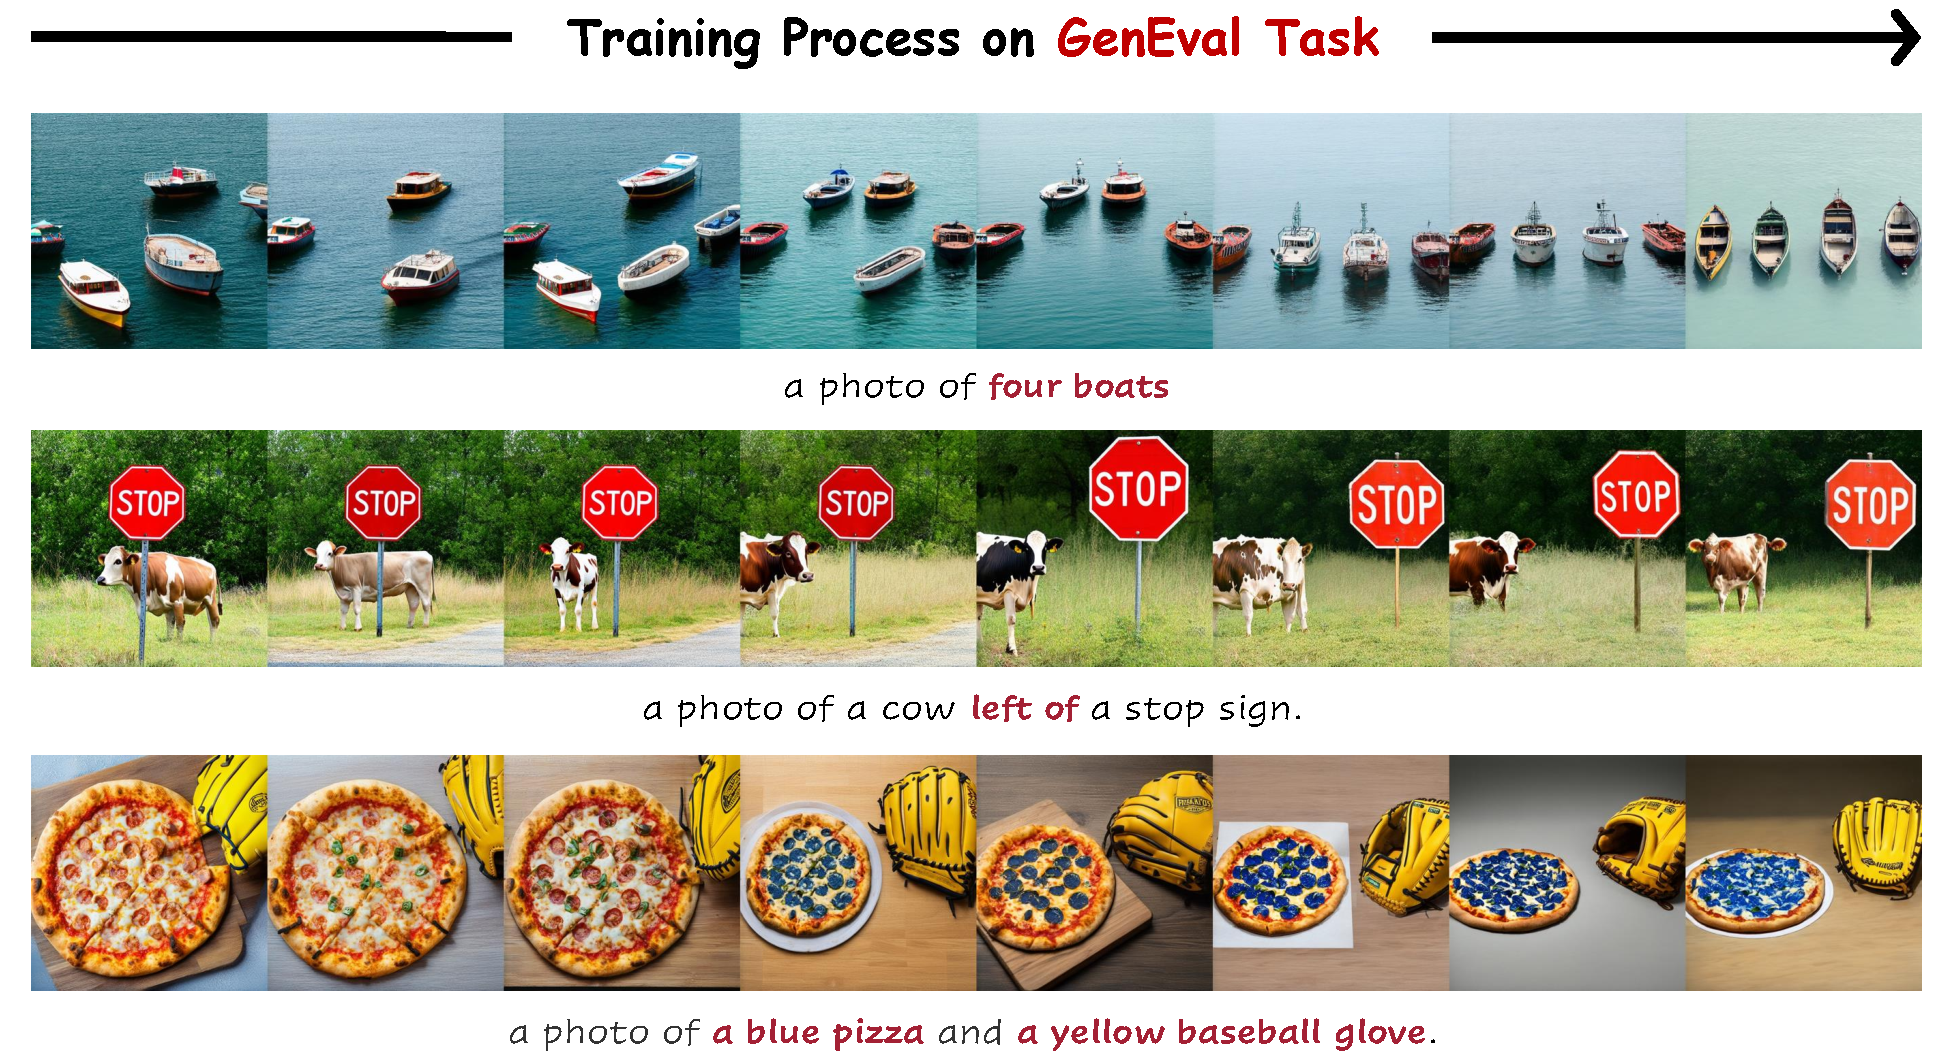
\includegraphics[width=\textwidth]{src/experiments/train_process/train_process_geneval.pdf}
\caption{We visualize the generated samples across successive training iterations during the optimization of SD3.5-Medium on the \textbf{GenEval} task.
}
\label{fig:evolve_qualitative_result_geneval}
\end{figure}

\begin{figure}[htbp]
\centering
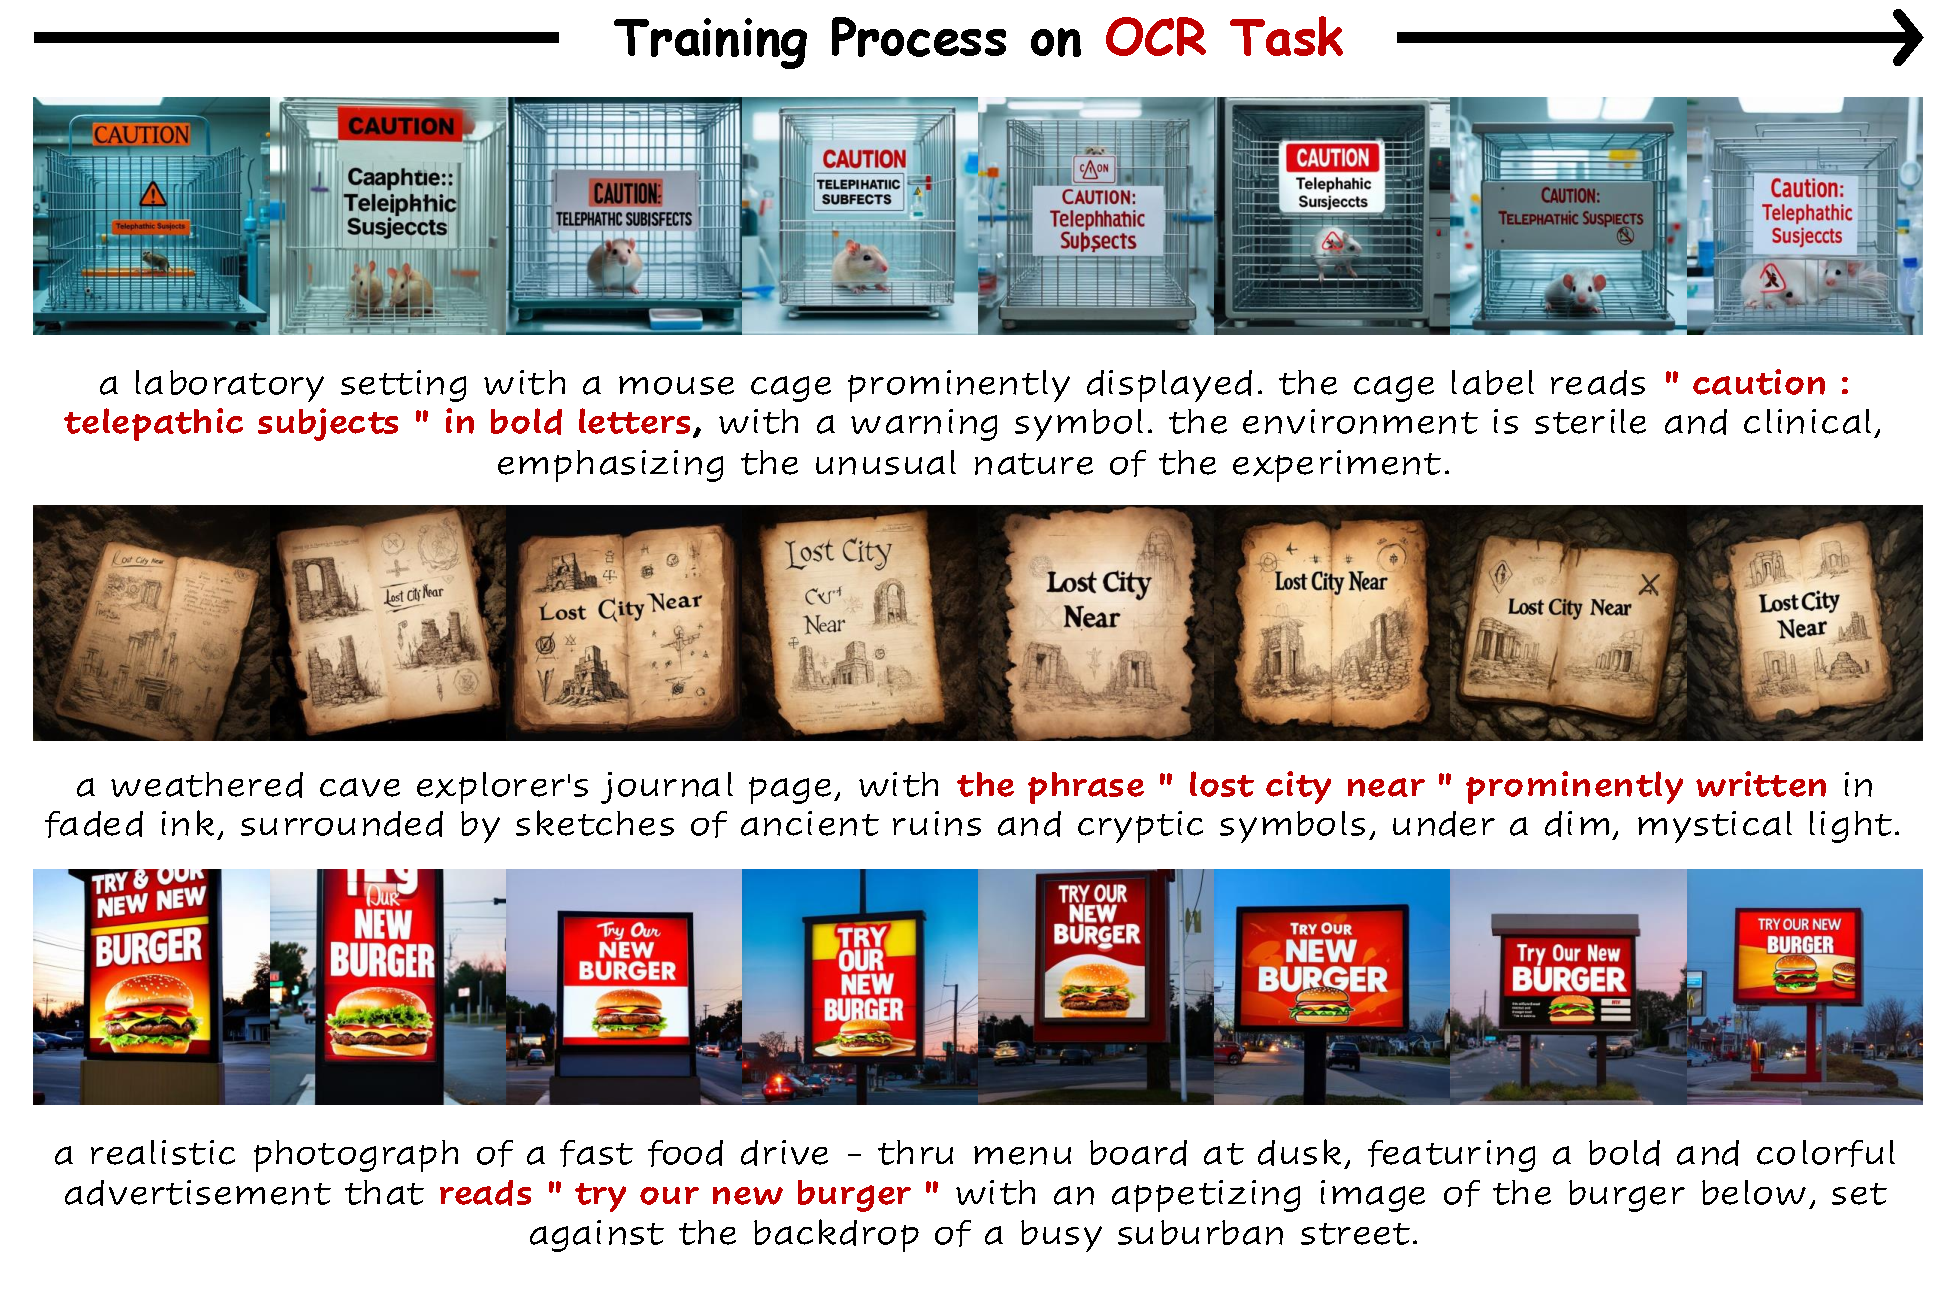
\includegraphics[width=\textwidth]{src/experiments/train_process/train_process_ocr.pdf}
\caption{We visualize the generated samples across successive training iterations during the optimization of SD3.5-Medium on the \textbf{OCR} task.
}
\label{fig:evolve_qualitative_result_ocr}
\end{figure}

\begin{figure}[htbp]
\centering
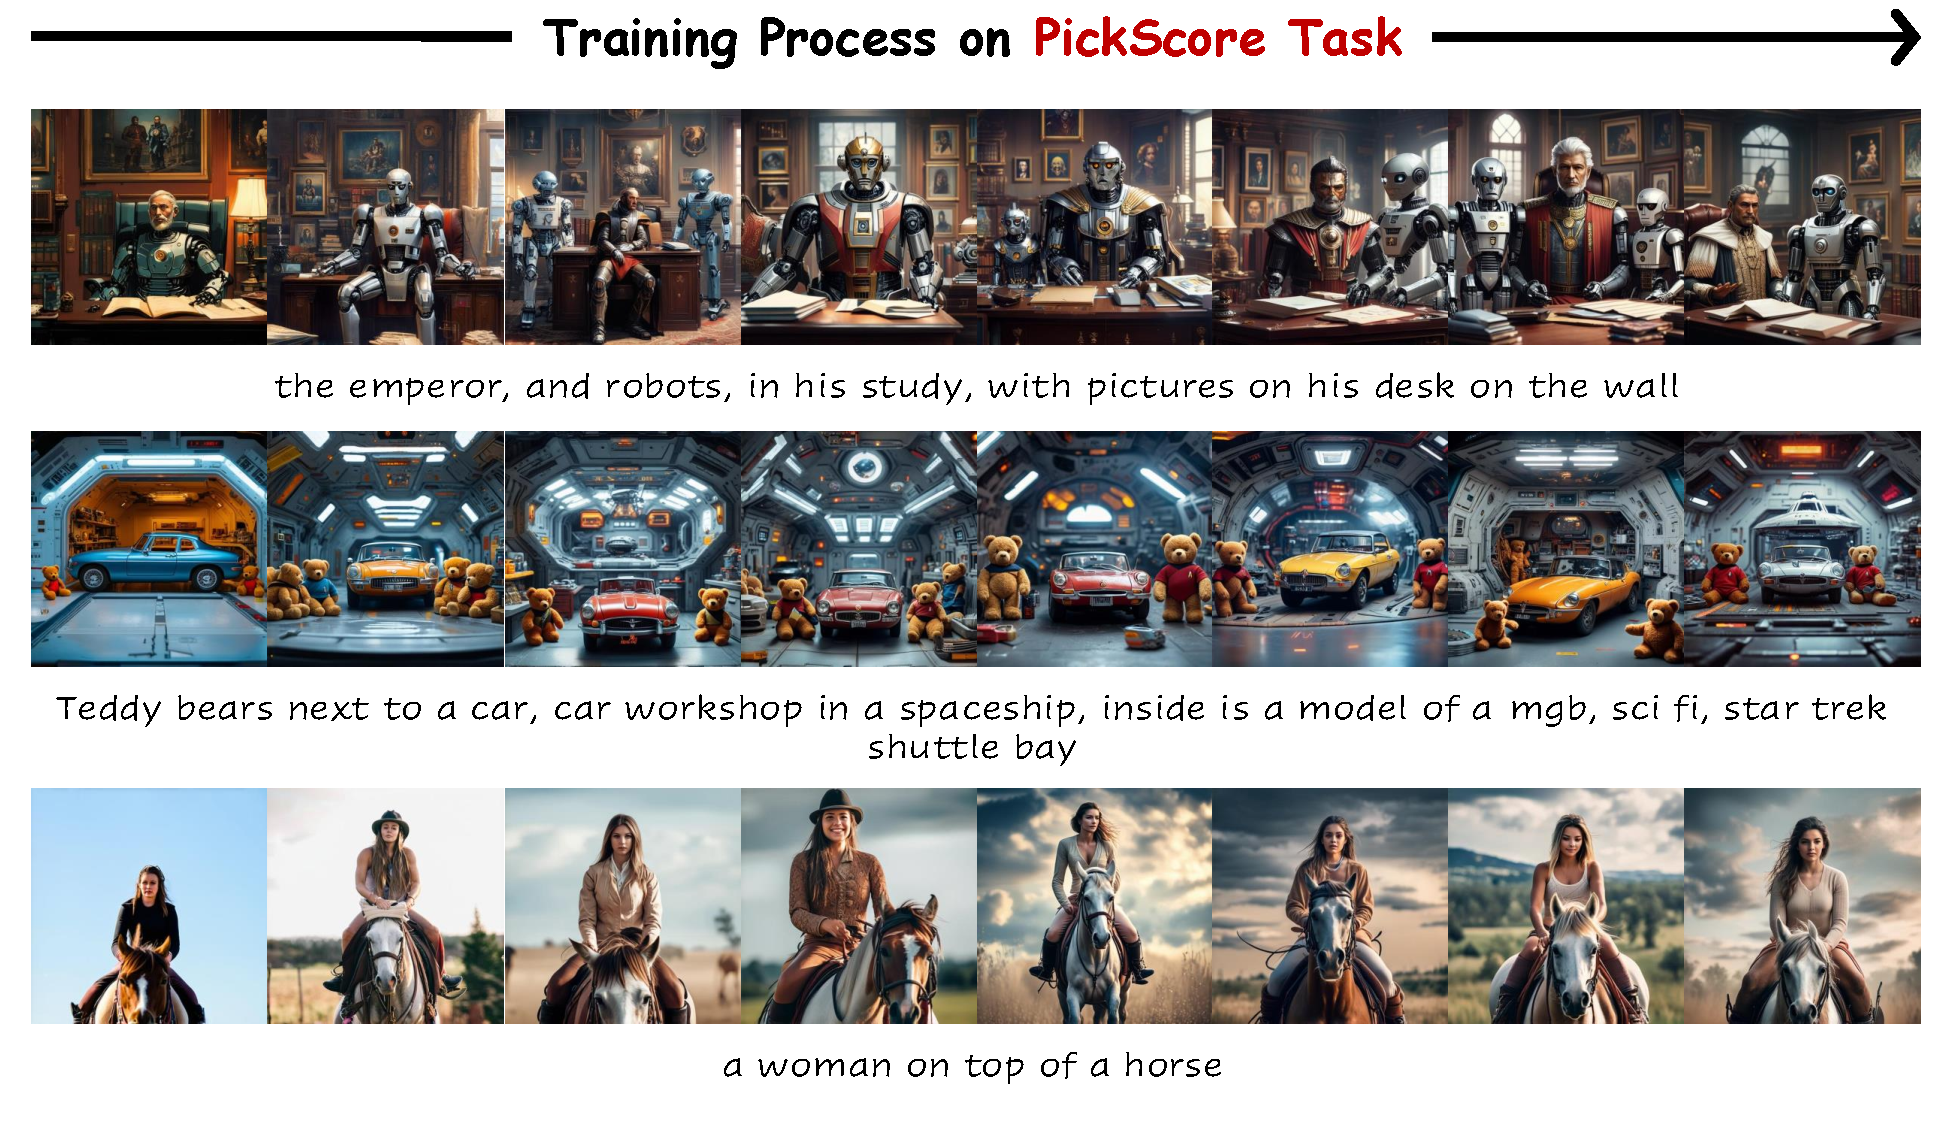
\includegraphics[width=\textwidth]{src/experiments/train_process/train_process_pickscore.pdf}
\caption{We visualize the generated samples across successive training iterations during the optimization of SD3.5-Medium on the \textbf{PickScore} task.
}
\label{fig:evolve_qualitative_result_picksore}
\end{figure}




\section{Training Sample Visualization with Denoising Reduction
}\label{app:sec:denoising_reduction_viz}

In this section, we compare images obtained with SDE sampling at various steps against those produced by ODE sampling, and offer an intuitive view of the denoising reduction strategy.
Figure~\ref{fig:denoising_reduction_viz} presents SD3.5-Medium samples under four inference settings:
(a) ODE sampling with 40 steps;
(b) SDE sampling with 40 steps;
(c) SDE sampling with 10 steps;
(d) SDE sampling with 5 steps.

The 40-step ODE and SDE runs yield visually indistinguishable images, confirming that our SDE sampler preserves quality. 
Shortening the SDE schedule to 10 and 5 steps introduces conspicuous artifacts, like color drift and fine details blur. 
Contrary to expectation that such low-quality samples might hinder optimization. it actually do just the opposite and accelerate optimization. 
Because Flow-GRPO relies on relative preferences, it still extracts a useful reward signal, while the shorter trajectories signifactly cut wall-clock time.
Consequently, Flow-GRPO with denoising reduction strategy converges more quickly on both layout-oriented benchmarks such as GenEval and quality-focused metrics such as PickScore, without sacrificing final performance.


\begin{figure}[htbp]
\centering
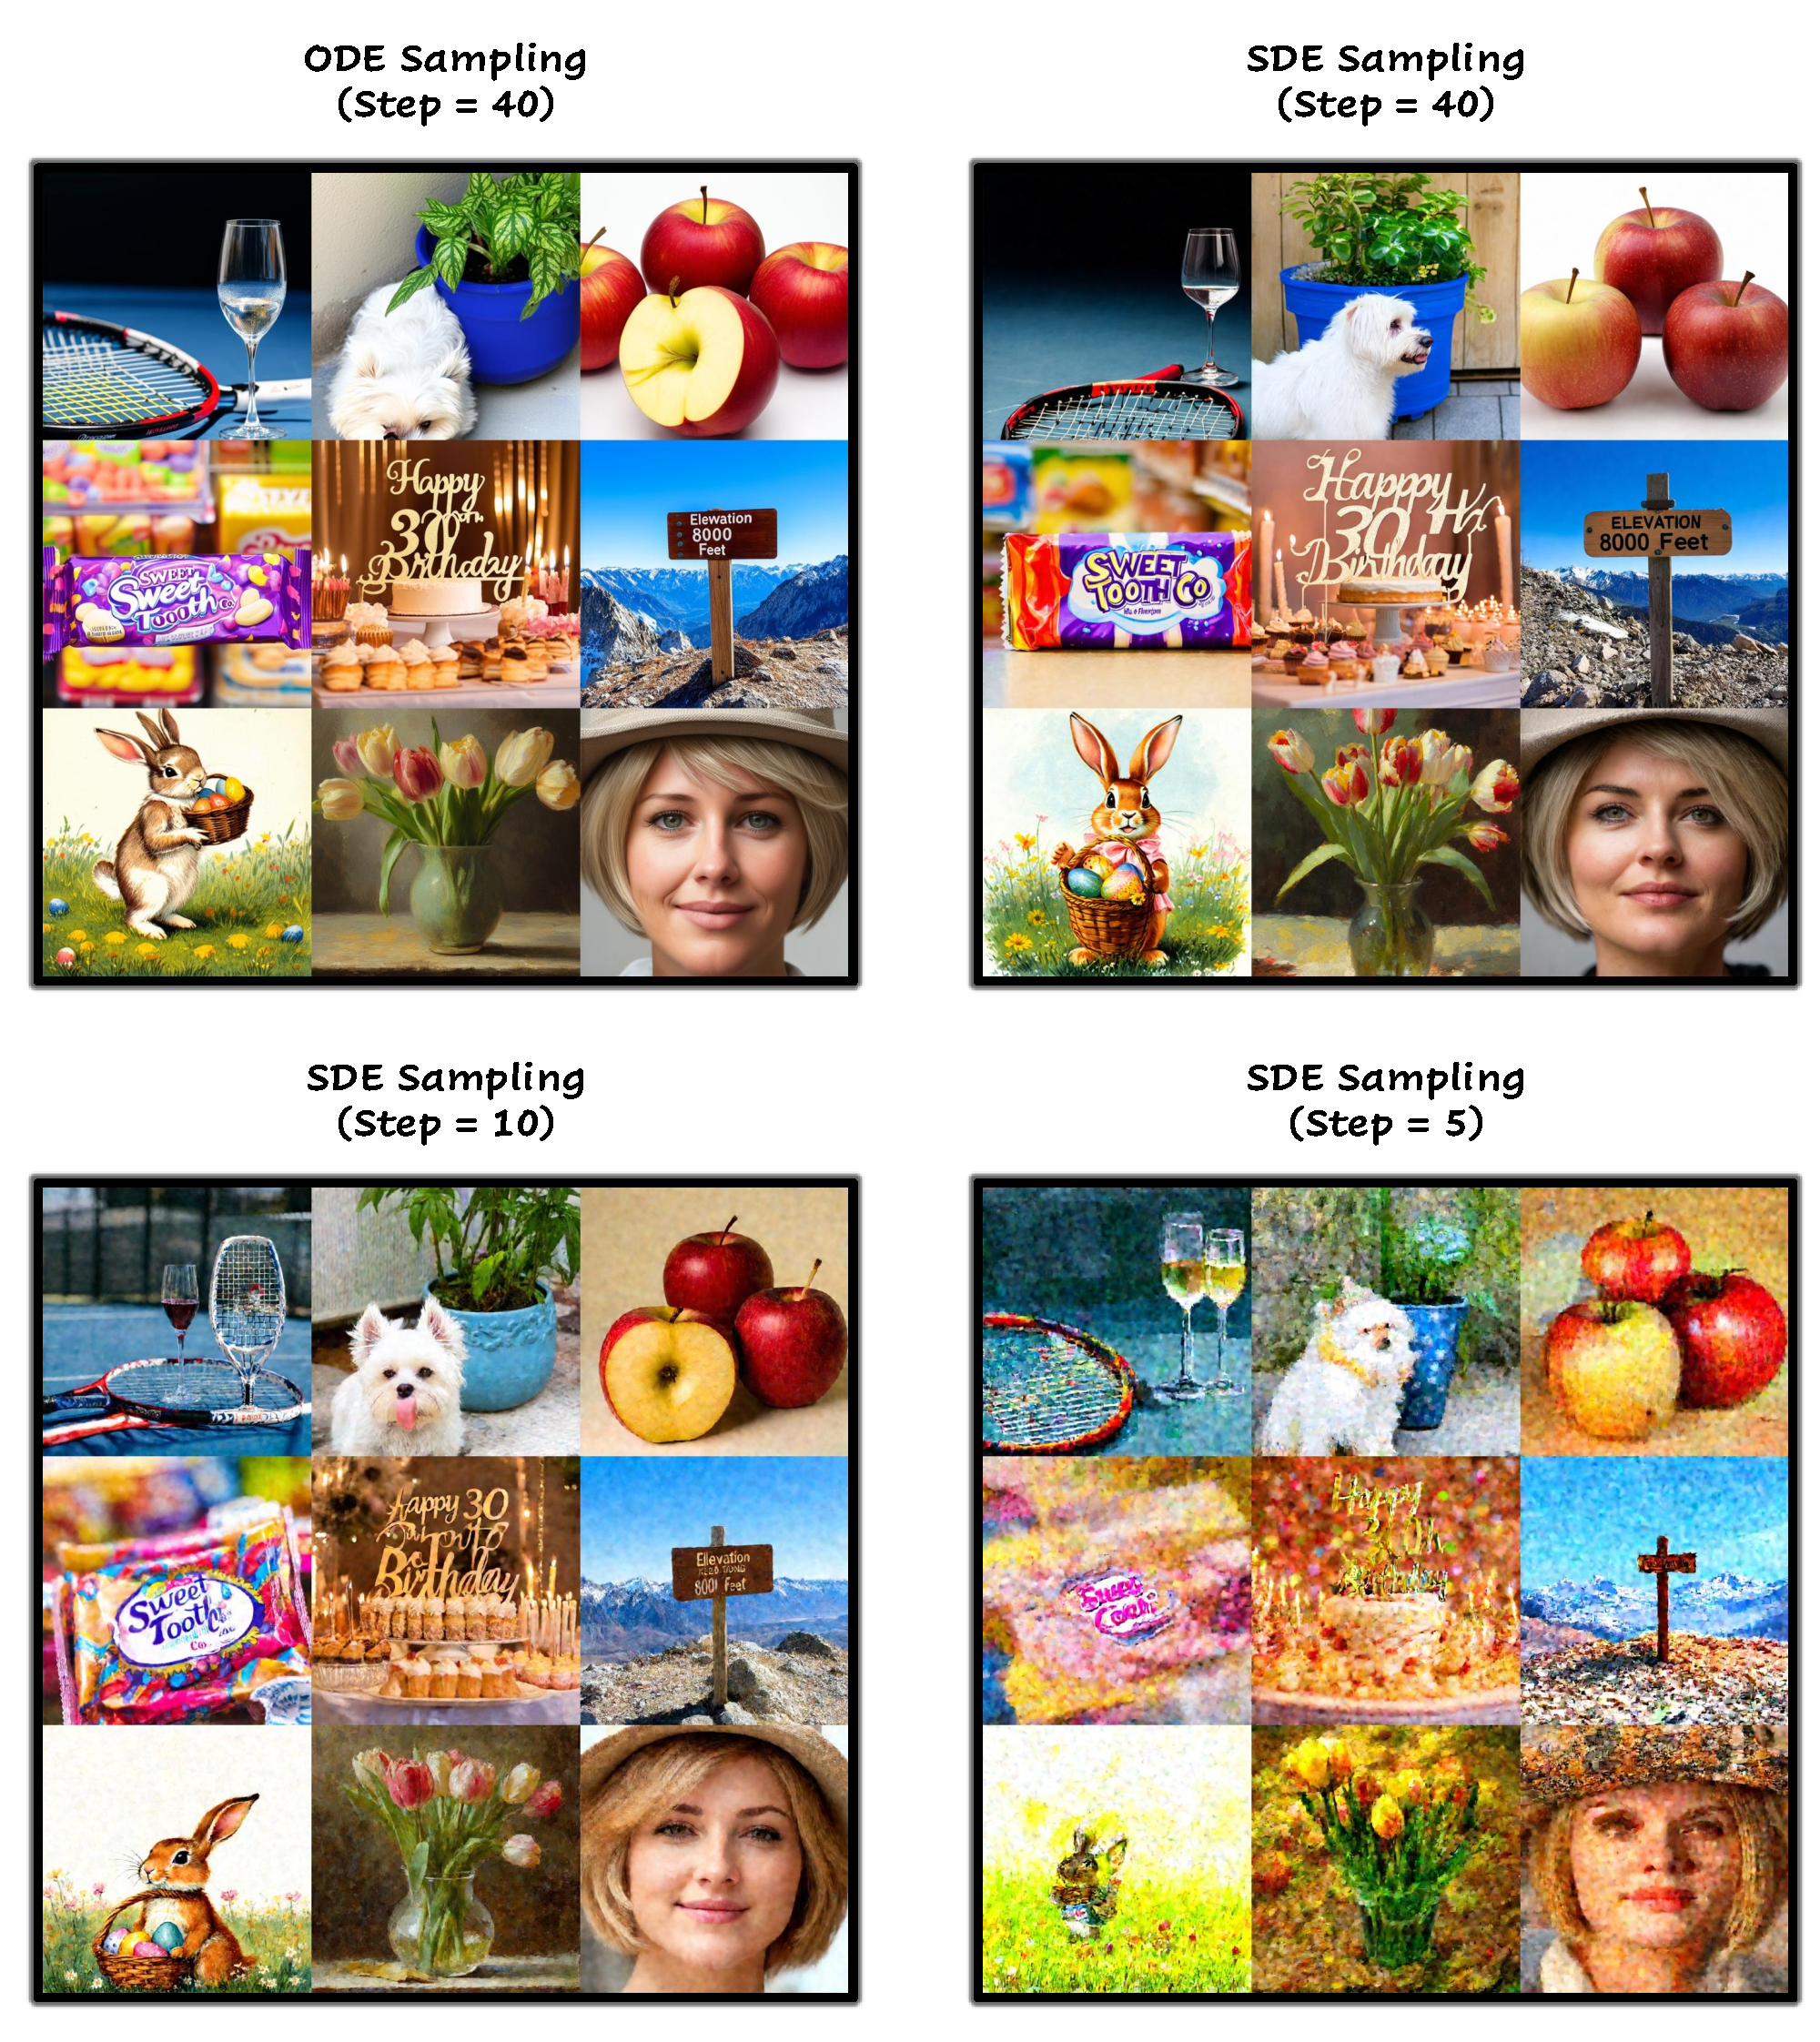
\includegraphics[width=\textwidth]{src/experiments/sampling_viz.pdf}
\caption{Visualization of training samples under difference inference settings.
}
\label{fig:denoising_reduction_viz}
\end{figure}
% \input{sections/appendix/generation_samples} 

% \input{sections/appendix/checklist}

% \clearpage
% \bibliography{
% references/flowpo,
% references/alignment, 
% references/search,
% references/proxy_tuning,
% references/models,
% references/benchmarks,
% references/others
% }

% \clearpage
% \iftoggle{isSubmission}{
%   \input{sections/check_list}
% }

\end{document}